\documentclass{book}
\usepackage[a4paper,top=2.5cm,bottom=2.5cm,left=2.5cm,right=2.5cm]{geometry}
\usepackage{makeidx}
\usepackage{natbib}
\usepackage{graphicx}
\usepackage{multicol}
\usepackage{float}
\usepackage{listings}
\usepackage{color}
\usepackage{ifthen}
\usepackage[table]{xcolor}
\usepackage{textcomp}
\usepackage{alltt}
\usepackage{ifpdf}
\ifpdf
\usepackage[pdftex,
            pagebackref=true,
            colorlinks=true,
            linkcolor=blue,
            unicode
           ]{hyperref}
\else
\usepackage[ps2pdf,
            pagebackref=true,
            colorlinks=true,
            linkcolor=blue,
            unicode
           ]{hyperref}
\usepackage{pspicture}
\fi
\usepackage[utf8]{inputenc}
\usepackage{mathptmx}
\usepackage[scaled=.90]{helvet}
\usepackage{courier}
\usepackage{sectsty}
\usepackage[titles]{tocloft}
\usepackage{doxygen}
\lstset{language=C++,inputencoding=utf8,basicstyle=\footnotesize,breaklines=true,breakatwhitespace=true,tabsize=8,numbers=left }
\makeindex
\setcounter{tocdepth}{3}
\renewcommand{\footrulewidth}{0.4pt}
\renewcommand{\familydefault}{\sfdefault}
\hfuzz=15pt
\setlength{\emergencystretch}{15pt}
\hbadness=750
\tolerance=750
\begin{document}
\hypersetup{pageanchor=false,citecolor=blue}
\begin{titlepage}
\vspace*{7cm}
\begin{center}
{\Large My Project \\[1ex]\large 1.\-0 }\\
\vspace*{1cm}
{\large Generated by Doxygen 1.8.0}\\
\vspace*{0.5cm}
{\small Tue Jun 12 2012 21:25:33}\\
\end{center}
\end{titlepage}
\clearemptydoublepage
\pagenumbering{roman}
\tableofcontents
\clearemptydoublepage
\pagenumbering{arabic}
\hypersetup{pageanchor=true,citecolor=blue}
\chapter{Namespace Index}
\section{Namespace List}
Here is a list of all namespaces with brief descriptions\-:\begin{DoxyCompactList}
\item\contentsline{section}{\hyperlink{namespace_ui}{Ui} }{\pageref{namespace_ui}}{}
\end{DoxyCompactList}

\chapter{Class Index}
\section{Class Hierarchy}
This inheritance list is sorted roughly, but not completely, alphabetically\-:\begin{DoxyCompactList}
\item \contentsline{section}{Constante}{\pageref{class_constante}}{}
\begin{DoxyCompactList}
\item \contentsline{section}{Expression}{\pageref{class_expression}}{}
\item \contentsline{section}{Nombre}{\pageref{class_nombre}}{}
\begin{DoxyCompactList}
\item \contentsline{section}{Nombre\-Complexe}{\pageref{class_nombre_complexe}}{}
\item \contentsline{section}{Nombre\-Non\-Complexe}{\pageref{class_nombre_non_complexe}}{}
\begin{DoxyCompactList}
\item \contentsline{section}{Entier}{\pageref{class_entier}}{}
\item \contentsline{section}{Rationnel}{\pageref{class_rationnel}}{}
\item \contentsline{section}{Reel}{\pageref{class_reel}}{}
\end{DoxyCompactList}
\end{DoxyCompactList}
\item \contentsline{section}{Operateur}{\pageref{class_operateur}}{}
\end{DoxyCompactList}
\item \contentsline{section}{Constante\-Factory}{\pageref{class_constante_factory}}{}
\item \contentsline{section}{Context}{\pageref{class_context}}{}
\item \contentsline{section}{Historique}{\pageref{class_historique}}{}
\begin{DoxyCompactList}
\item \contentsline{section}{Historique\-Operateur\-Binaire}{\pageref{class_historique_operateur_binaire}}{}
\item \contentsline{section}{Historique\-Operateur\-Push}{\pageref{class_historique_operateur_push}}{}
\item \contentsline{section}{Historique\-Operateur\-Sum\-Mean}{\pageref{class_historique_operateur_sum_mean}}{}
\item \contentsline{section}{Historique\-Operateur\-Swap}{\pageref{class_historique_operateur_swap}}{}
\item \contentsline{section}{Historique\-Operateur\-Unaire}{\pageref{class_historique_operateur_unaire}}{}
\end{DoxyCompactList}
\item \contentsline{section}{Log\-Message}{\pageref{class_log_message}}{}
\item \contentsline{section}{Log\-System}{\pageref{class_log_system}}{}
\item \contentsline{section}{Main\-Window}{\pageref{class_main_window}}{}
\item \contentsline{section}{Pile}{\pageref{class_pile}}{}
\item \contentsline{section}{Settings}{\pageref{class_settings}}{}
\end{DoxyCompactList}

\chapter{Class Index}
\section{Class List}
Here are the classes, structs, unions and interfaces with brief descriptions\-:\begin{DoxyCompactList}
\item\contentsline{section}{\hyperlink{class_constante}{Constante} \\*Interface (utilisant le design pattern composite) permettant de g�rer les diff�rents types de valeurs qui peuvent �tre empil�es sur la pile }{\pageref{class_constante}}{}
\item\contentsline{section}{\hyperlink{class_constante_factory}{Constante\-Factory} \\*Classe (utilisant le Design Pattern Factory) permettant d'instancier des objets de type \hyperlink{class_constante}{Constante} }{\pageref{class_constante_factory}}{}
\item\contentsline{section}{\hyperlink{class_context}{Context} \\*Classe (utilisant le Design Pattern Singleton) permettant de g�rer l'�criture du context afin de pouvoir le recharger lors de l'ouverture de l'application }{\pageref{class_context}}{}
\item\contentsline{section}{\hyperlink{class_entier}{Entier} \\*Classe impl�mentant l'interface de \hyperlink{class_nombre_non_complexe}{Nombre\-Non\-Complexe} et permettant de g�rer des constantes de type entier }{\pageref{class_entier}}{}
\item\contentsline{section}{\hyperlink{class_expression}{Expression} \\*Classe impl�mentant l'interface de \hyperlink{class_constante}{Constante} et permettant la gestion d'un expression }{\pageref{class_expression}}{}
\item\contentsline{section}{\hyperlink{class_historique}{Historique} \\*Classe (utilisant le design pattern command) abstraite permettant de g�rer des objets de type \hyperlink{class_historique}{Historique} }{\pageref{class_historique}}{}
\item\contentsline{section}{\hyperlink{class_historique_operateur_binaire}{Historique\-Operateur\-Binaire} \\*Classe impl�mentant l'interface \hyperlink{class_historique}{Historique} et permettant de g�rer l'historique de toute les commandes binaires }{\pageref{class_historique_operateur_binaire}}{}
\item\contentsline{section}{\hyperlink{class_historique_operateur_push}{Historique\-Operateur\-Push} \\*Classe impl�mentant l'interface \hyperlink{class_historique}{Historique} et permettant de g�rer l'historique de tous les push }{\pageref{class_historique_operateur_push}}{}
\item\contentsline{section}{\hyperlink{class_historique_operateur_sum_mean}{Historique\-Operateur\-Sum\-Mean} \\*Classe impl�mentant l'interface \hyperlink{class_historique}{Historique} et permettant de g�rer l'historique des commandes \char`\"{}sum\char`\"{} et \char`\"{}mean\char`\"{} }{\pageref{class_historique_operateur_sum_mean}}{}
\item\contentsline{section}{\hyperlink{class_historique_operateur_swap}{Historique\-Operateur\-Swap} \\*Classe impl�mentant l'interface \hyperlink{class_historique}{Historique} et permettant de g�rer l'historique de la commande swap }{\pageref{class_historique_operateur_swap}}{}
\item\contentsline{section}{\hyperlink{class_historique_operateur_unaire}{Historique\-Operateur\-Unaire} \\*Classe impl�mentant l'interface \hyperlink{class_historique}{Historique} et permettant de g�rer l'historique des commandes unaires }{\pageref{class_historique_operateur_unaire}}{}
\item\contentsline{section}{\hyperlink{class_log_message}{Log\-Message} \\*Classe permettant de g�rer un message de Log (son contenu et son degre d'importance) }{\pageref{class_log_message}}{}
\item\contentsline{section}{\hyperlink{class_log_system}{Log\-System} \\*Classe (utilisant le Design Pattern Singleton) permettant de g�rer l'�criture des messages de log dans le fichier correspondant }{\pageref{class_log_system}}{}
\item\contentsline{section}{\hyperlink{class_main_window}{Main\-Window} \\*Classe (utilisant le Design Pattern Singleton) permettant de g�rer l'interface de la calculatrice, ainsi que les interactions entre celle-\/ci et les classes associ�es }{\pageref{class_main_window}}{}
\item\contentsline{section}{\hyperlink{class_nombre}{Nombre} \\*Classe qui �tend l'interface \hyperlink{class_constante}{Constante} pour regrouper tout les valeurs de type num�rique sous cette classe et �galement de proposer les diff�rentes op�rations sp�cifiques aux nombres (op�rations arithm�tiques, etc) }{\pageref{class_nombre}}{}
\item\contentsline{section}{\hyperlink{class_nombre_complexe}{Nombre\-Complexe} \\*Classe impl�mentant l'interface \hyperlink{class_nombre}{Nombre} et permettant de g�rer des constantes de type complexe }{\pageref{class_nombre_complexe}}{}
\item\contentsline{section}{\hyperlink{class_nombre_non_complexe}{Nombre\-Non\-Complexe} \\*Classe qui �tend l'interface \hyperlink{class_nombre}{Nombre} et permettant de g�rer des constantes de type non complexe (\hyperlink{class_entier}{Entier}, \hyperlink{class_rationnel}{Rationnel}, \hyperlink{class_reel}{Reel}) }{\pageref{class_nombre_non_complexe}}{}
\item\contentsline{section}{\hyperlink{class_operateur}{Operateur} \\*Classe (utilisant le design pattern strategy) impl�mentant l'interface de \hyperlink{class_constante}{Constante} et permettant de g�rer les constantes de type op�rateur (+,-\/,/,$\ast$, sin, cos, etc...) }{\pageref{class_operateur}}{}
\item\contentsline{section}{\hyperlink{class_pile}{Pile} \\*Classe permettant de g�rer la pile d'�l�ments et �galement l'historique de cette pile }{\pageref{class_pile}}{}
\item\contentsline{section}{\hyperlink{class_rationnel}{Rationnel} \\*Classe impl�mentant l'interface de \hyperlink{class_nombre_non_complexe}{Nombre\-Non\-Complexe} et permettant de g�rer les constantes de type rationnel }{\pageref{class_rationnel}}{}
\item\contentsline{section}{\hyperlink{class_reel}{Reel} \\*Classe impl�mentant l'interface de \hyperlink{class_nombre_non_complexe}{Nombre\-Non\-Complexe} et permettant de g�rer les constantes de type reel }{\pageref{class_reel}}{}
\item\contentsline{section}{\hyperlink{class_settings}{Settings} \\*Classe (utilisant le Design Pattern Singleton) permettant de gerer les param�tres de la calculatrice (utilisee dans le cadre de la sauvegarde de contexte notamment) }{\pageref{class_settings}}{}
\end{DoxyCompactList}

\chapter{File Index}
\section{File List}
Here is a list of all files with brief descriptions\-:\begin{DoxyCompactList}
\item\contentsline{section}{\hyperlink{constante_8cpp}{constante.\-cpp} }{\pageref{constante_8cpp}}{}
\item\contentsline{section}{\hyperlink{constante_8h}{constante.\-h} }{\pageref{constante_8h}}{}
\item\contentsline{section}{\hyperlink{constantefactory_8cpp}{constantefactory.\-cpp} }{\pageref{constantefactory_8cpp}}{}
\item\contentsline{section}{\hyperlink{constante_factory_8h}{constante\-Factory.\-h} }{\pageref{constante_factory_8h}}{}
\item\contentsline{section}{\hyperlink{context_8cpp}{context.\-cpp} }{\pageref{context_8cpp}}{}
\item\contentsline{section}{\hyperlink{context_8h}{context.\-h} }{\pageref{context_8h}}{}
\item\contentsline{section}{\hyperlink{entier_8cpp}{entier.\-cpp} }{\pageref{entier_8cpp}}{}
\item\contentsline{section}{\hyperlink{entier_8h}{entier.\-h} }{\pageref{entier_8h}}{}
\item\contentsline{section}{\hyperlink{expression_8cpp}{expression.\-cpp} }{\pageref{expression_8cpp}}{}
\item\contentsline{section}{\hyperlink{expression_8h}{expression.\-h} }{\pageref{expression_8h}}{}
\item\contentsline{section}{\hyperlink{historique_8cpp}{historique.\-cpp} }{\pageref{historique_8cpp}}{}
\item\contentsline{section}{\hyperlink{historique_8h}{historique.\-h} }{\pageref{historique_8h}}{}
\item\contentsline{section}{\hyperlink{historique_operateur_binaire_8cpp}{historique\-Operateur\-Binaire.\-cpp} }{\pageref{historique_operateur_binaire_8cpp}}{}
\item\contentsline{section}{\hyperlink{historique_operateur_binaire_8h}{historique\-Operateur\-Binaire.\-h} }{\pageref{historique_operateur_binaire_8h}}{}
\item\contentsline{section}{\hyperlink{historique_operateur_push_8cpp}{historique\-Operateur\-Push.\-cpp} }{\pageref{historique_operateur_push_8cpp}}{}
\item\contentsline{section}{\hyperlink{historique_operateur_push_8h}{historique\-Operateur\-Push.\-h} }{\pageref{historique_operateur_push_8h}}{}
\item\contentsline{section}{\hyperlink{historique_operateur_sum_mean_8cpp}{historique\-Operateur\-Sum\-Mean.\-cpp} }{\pageref{historique_operateur_sum_mean_8cpp}}{}
\item\contentsline{section}{\hyperlink{historique_operateur_sum_mean_8h}{historique\-Operateur\-Sum\-Mean.\-h} }{\pageref{historique_operateur_sum_mean_8h}}{}
\item\contentsline{section}{\hyperlink{historique_operateur_swap_8cpp}{historique\-Operateur\-Swap.\-cpp} }{\pageref{historique_operateur_swap_8cpp}}{}
\item\contentsline{section}{\hyperlink{historique_operateur_swap_8h}{historique\-Operateur\-Swap.\-h} }{\pageref{historique_operateur_swap_8h}}{}
\item\contentsline{section}{\hyperlink{historique_operateur_unaire_8cpp}{historique\-Operateur\-Unaire.\-cpp} }{\pageref{historique_operateur_unaire_8cpp}}{}
\item\contentsline{section}{\hyperlink{historique_operateur_unaire_8h}{historique\-Operateur\-Unaire.\-h} }{\pageref{historique_operateur_unaire_8h}}{}
\item\contentsline{section}{\hyperlink{log_message_8cpp}{log\-Message.\-cpp} }{\pageref{log_message_8cpp}}{}
\item\contentsline{section}{\hyperlink{log_message_8h}{log\-Message.\-h} \\*Classe permettant de gerer un message de log (son contenu et son degre d'importance) }{\pageref{log_message_8h}}{}
\item\contentsline{section}{\hyperlink{log_system_8cpp}{log\-System.\-cpp} \\*Classe permettant de gerer les logs du programme }{\pageref{log_system_8cpp}}{}
\item\contentsline{section}{\hyperlink{log_system_8h}{log\-System.\-h} }{\pageref{log_system_8h}}{}
\item\contentsline{section}{\hyperlink{main_8cpp}{main.\-cpp} }{\pageref{main_8cpp}}{}
\item\contentsline{section}{\hyperlink{mainwindow_8cpp}{mainwindow.\-cpp} }{\pageref{mainwindow_8cpp}}{}
\item\contentsline{section}{\hyperlink{mainwindow_8h}{mainwindow.\-h} }{\pageref{mainwindow_8h}}{}
\item\contentsline{section}{\hyperlink{nombre_8cpp}{nombre.\-cpp} }{\pageref{nombre_8cpp}}{}
\item\contentsline{section}{\hyperlink{nombre_8h}{nombre.\-h} }{\pageref{nombre_8h}}{}
\item\contentsline{section}{\hyperlink{nombre_complexe_8cpp}{nombre\-Complexe.\-cpp} }{\pageref{nombre_complexe_8cpp}}{}
\item\contentsline{section}{\hyperlink{nombre_complexe_8h}{nombre\-Complexe.\-h} }{\pageref{nombre_complexe_8h}}{}
\item\contentsline{section}{\hyperlink{nombre_non_complexe_8cpp}{nombre\-Non\-Complexe.\-cpp} }{\pageref{nombre_non_complexe_8cpp}}{}
\item\contentsline{section}{\hyperlink{nombre_non_complexe_8h}{nombre\-Non\-Complexe.\-h} }{\pageref{nombre_non_complexe_8h}}{}
\item\contentsline{section}{\hyperlink{operateur_8cpp}{operateur.\-cpp} }{\pageref{operateur_8cpp}}{}
\item\contentsline{section}{\hyperlink{operateur_8h}{operateur.\-h} }{\pageref{operateur_8h}}{}
\item\contentsline{section}{\hyperlink{pile_8cpp}{pile.\-cpp} }{\pageref{pile_8cpp}}{}
\item\contentsline{section}{\hyperlink{pile_8h}{pile.\-h} }{\pageref{pile_8h}}{}
\item\contentsline{section}{\hyperlink{rationnel_8cpp}{rationnel.\-cpp} }{\pageref{rationnel_8cpp}}{}
\item\contentsline{section}{\hyperlink{rationnel_8h}{rationnel.\-h} }{\pageref{rationnel_8h}}{}
\item\contentsline{section}{\hyperlink{reel_8cpp}{reel.\-cpp} }{\pageref{reel_8cpp}}{}
\item\contentsline{section}{\hyperlink{reel_8h}{reel.\-h} }{\pageref{reel_8h}}{}
\item\contentsline{section}{\hyperlink{settings_8cpp}{settings.\-cpp} }{\pageref{settings_8cpp}}{}
\item\contentsline{section}{\hyperlink{settings_8h}{settings.\-h} \\*Classe permettant de gerer les param�tres de la calculatrice }{\pageref{settings_8h}}{}
\end{DoxyCompactList}

\chapter{Namespace Documentation}
\hypertarget{namespace_ui}{\section{Ui Namespace Reference}
\label{namespace_ui}\index{Ui@{Ui}}
}

\chapter{Class Documentation}
\hypertarget{class_constante}{\section{Constante Class Reference}
\label{class_constante}\index{Constante@{Constante}}
}


Interface (utilisant le design pattern composite) permettant de g�rer les diff�rents types de valeurs qui peuvent �tre empil�es sur la pile.  




{\ttfamily \#include $<$constante.\-h$>$}

Inheritance diagram for Constante\-:\begin{figure}[H]
\begin{center}
\leavevmode
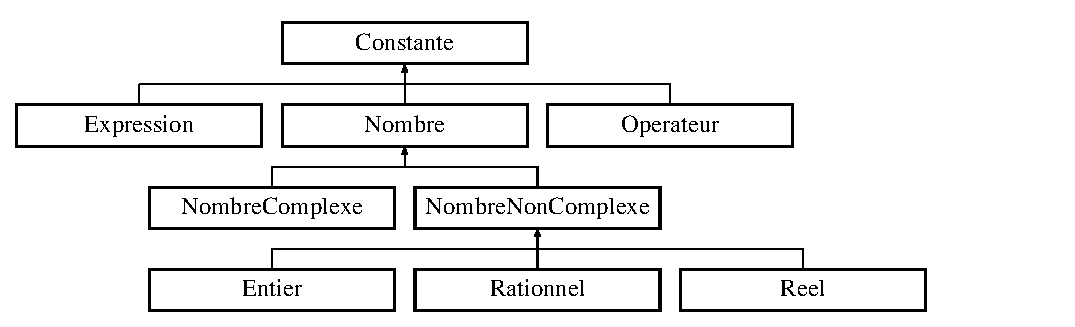
\includegraphics[height=3.943662cm]{class_constante}
\end{center}
\end{figure}
\subsection*{Public Member Functions}
\begin{DoxyCompactItemize}
\item 
virtual \hyperlink{class_constante_af747f270ad3d50813786a1b013bac959}{$\sim$\-Constante} ()
\begin{DoxyCompactList}\small\item\em Destructeur de l'instance de la classe \hyperlink{class_constante}{Constante}. \end{DoxyCompactList}\item 
virtual \hyperlink{class_constante}{Constante} $\ast$ \hyperlink{class_constante_a5769ea385161e02bd2d1bcadefc2c510}{clone} () const =0
\begin{DoxyCompactList}\small\item\em M�thode permettant de cloner une constante. \end{DoxyCompactList}\item 
virtual Q\-String \hyperlink{class_constante_ad5ea6850196ee9f86b74c74009a87ab1}{to\-String} () const =0
\begin{DoxyCompactList}\small\item\em Fonction permettant de renvoyer une chaine comprenant la valuation de la constante associ�, cette fonction est utilis�e dans le cadre de l'affichage des constantes dans la pile. \end{DoxyCompactList}\end{DoxyCompactItemize}


\subsection{Detailed Description}
Interface (utilisant le design pattern composite) permettant de g�rer les diff�rents types de valeurs qui peuvent �tre empil�es sur la pile. 

Definition at line 18 of file constante.\-h.



\subsection{Constructor \& Destructor Documentation}
\hypertarget{class_constante_af747f270ad3d50813786a1b013bac959}{\index{Constante@{Constante}!$\sim$\-Constante@{$\sim$\-Constante}}
\index{$\sim$\-Constante@{$\sim$\-Constante}!Constante@{Constante}}
\subsubsection[{$\sim$\-Constante}]{\setlength{\rightskip}{0pt plus 5cm}virtual {\bf Constante\-::$\sim$\-Constante} (
\begin{DoxyParamCaption}
{}
\end{DoxyParamCaption}
)\hspace{0.3cm}{\ttfamily  \mbox{[}inline, virtual\mbox{]}}}}\label{class_constante_af747f270ad3d50813786a1b013bac959}


Destructeur de l'instance de la classe \hyperlink{class_constante}{Constante}. 



Definition at line 24 of file constante.\-h.



\subsection{Member Function Documentation}
\hypertarget{class_constante_a5769ea385161e02bd2d1bcadefc2c510}{\index{Constante@{Constante}!clone@{clone}}
\index{clone@{clone}!Constante@{Constante}}
\subsubsection[{clone}]{\setlength{\rightskip}{0pt plus 5cm}virtual {\bf Constante}$\ast$ {\bf Constante\-::clone} (
\begin{DoxyParamCaption}
{}
\end{DoxyParamCaption}
) const\hspace{0.3cm}{\ttfamily  \mbox{[}pure virtual\mbox{]}}}}\label{class_constante_a5769ea385161e02bd2d1bcadefc2c510}


M�thode permettant de cloner une constante. 


\begin{DoxyParams}{Parameters}
{\em Le} & pointeur vers la constante clon�e \\
\hline
\end{DoxyParams}


Implemented in \hyperlink{class_rationnel_a422ec3e0c4465d08c4e9deceda6c442c}{Rationnel}, \hyperlink{class_reel_ab53c7d10a93c702bd7ccde897fc396df}{Reel}, \hyperlink{class_entier_aca1eef6372c8d74274bffd435888ef57}{Entier}, \hyperlink{class_operateur_a77814d91250ee0c65501cea7d135b76c}{Operateur}, \hyperlink{class_nombre_complexe_a22709b554d12923c00e2b8b984143165}{Nombre\-Complexe}, and \hyperlink{class_expression_ad357e8bb1174b3582833ebcbf6d6e232}{Expression}.

\hypertarget{class_constante_ad5ea6850196ee9f86b74c74009a87ab1}{\index{Constante@{Constante}!to\-String@{to\-String}}
\index{to\-String@{to\-String}!Constante@{Constante}}
\subsubsection[{to\-String}]{\setlength{\rightskip}{0pt plus 5cm}virtual Q\-String {\bf Constante\-::to\-String} (
\begin{DoxyParamCaption}
{}
\end{DoxyParamCaption}
) const\hspace{0.3cm}{\ttfamily  \mbox{[}pure virtual\mbox{]}}}}\label{class_constante_ad5ea6850196ee9f86b74c74009a87ab1}


Fonction permettant de renvoyer une chaine comprenant la valuation de la constante associ�, cette fonction est utilis�e dans le cadre de l'affichage des constantes dans la pile. 

\begin{DoxyReturn}{Returns}
La chaine � afficher dans la pile 
\end{DoxyReturn}


Implemented in \hyperlink{class_nombre_complexe_a2b02fa6dc1f9f3d889f69db7a9143f84}{Nombre\-Complexe}, \hyperlink{class_rationnel_a41bc89d21ce161818f67ccfe296766c0}{Rationnel}, \hyperlink{class_entier_aa960356dfeae8af6dfa2cd25136a1a6f}{Entier}, \hyperlink{class_reel_a990e8324822ba3dbc64fc7ff727411e2}{Reel}, \hyperlink{class_operateur_ad49ae9c67adcd3af3a9be0e2bc13c629}{Operateur}, and \hyperlink{class_expression_a60e6e305cdd8e878df2e3081ae15a4d0}{Expression}.



The documentation for this class was generated from the following file\-:\begin{DoxyCompactItemize}
\item 
\hyperlink{constante_8h}{constante.\-h}\end{DoxyCompactItemize}

\hypertarget{class_constante_factory}{\section{Constante\-Factory Class Reference}
\label{class_constante_factory}\index{Constante\-Factory@{Constante\-Factory}}
}


Classe (utilisant le Design Pattern Factory) permettant d'instancier des objets de type \hyperlink{class_constante}{Constante}.  




{\ttfamily \#include $<$constante\-Factory.\-h$>$}

\subsection*{Static Public Member Functions}
\begin{DoxyCompactItemize}
\item 
static \hyperlink{class_constante}{Constante} $\ast$ \hyperlink{class_constante_factory_aa8bd9c782cff8752955f88b2c6fcb475}{get\-Constante} (const Q\-String \&str)  throw (\-Log\-Message)
\begin{DoxyCompactList}\small\item\em M�thode permettant de cr�e un objet de type \hyperlink{class_constante}{en lui passant une Q\-String en parametre. }\end{DoxyCompactList}\end{DoxyCompactItemize}


\subsection{Detailed Description}
Classe (utilisant le Design Pattern Factory) permettant d'instancier des objets de type \hyperlink{class_constante}{Constante}. 

Definition at line 19 of file constante\-Factory.\-h.



\subsection{Member Function Documentation}
\hypertarget{class_constante_factory_aa8bd9c782cff8752955f88b2c6fcb475}{\index{Constante\-Factory@{Constante\-Factory}!get\-Constante@{get\-Constante}}
\index{get\-Constante@{get\-Constante}!ConstanteFactory@{Constante\-Factory}}
\subsubsection[{get\-Constante}]{\setlength{\rightskip}{0pt plus 5cm}{\bf Constante} $\ast$ {\bf Constante\-Factory\-::get\-Constante} (
\begin{DoxyParamCaption}
\item[{const Q\-String \&}]{str}
\end{DoxyParamCaption}
)  throw ({\bf Log\-Message})\hspace{0.3cm}{\ttfamily  \mbox{[}static\mbox{]}}}}\label{class_constante_factory_aa8bd9c782cff8752955f88b2c6fcb475}


M�thode permettant de cr�e un objet de type \hyperlink{class_constante}{en lui passant une Q\-String en parametre. }


\begin{DoxyParams}{Parameters}
{\em str} & La chaine � convertir en \hyperlink{class_constante}{Constante} \\
\hline
\end{DoxyParams}


Definition at line 10 of file constantefactory.\-cpp.



The documentation for this class was generated from the following files\-:\begin{DoxyCompactItemize}
\item 
\hyperlink{constante_factory_8h}{constante\-Factory.\-h}\item 
\hyperlink{constantefactory_8cpp}{constantefactory.\-cpp}\end{DoxyCompactItemize}

\hypertarget{class_context}{\section{Context Class Reference}
\label{class_context}\index{Context@{Context}}
}


Classe (utilisant le Design Pattern Singleton) permettant de g�rer l'�criture du context afin de pouvoir le recharger lors de l'ouverture de l'application.  




{\ttfamily \#include $<$context.\-h$>$}

\subsection*{Public Member Functions}
\begin{DoxyCompactItemize}
\item 
void \hyperlink{class_context_ae81f5eb81363ce52af77a029e62cbf7e}{sauvegarde\-Context} ()
\begin{DoxyCompactList}\small\item\em M�thode permettant de stocker le contexte en m�moire afin de pouvoir le recharger apr�s. \end{DoxyCompactList}\item 
void \hyperlink{class_context_a8e6cf6dafb4a736dd08b906cd38e6e0e}{charger\-Context} ()  throw (\-Log\-Message)
\begin{DoxyCompactList}\small\item\em M�thode permettant de charger le contexte afin de restaurer les param�tres de la calculatrice et l'�tat de la pile. \end{DoxyCompactList}\end{DoxyCompactItemize}
\subsection*{Static Public Member Functions}
\begin{DoxyCompactItemize}
\item 
static \hyperlink{class_context}{Context} $\ast$ \hyperlink{class_context_ad0c275450890b2a68186ad6d0095874b}{get\-Instance} ()
\begin{DoxyCompactList}\small\item\em Getter de l'unique instance de \hyperlink{class_context}{Context}, si elle existe pas, on la cr�e. \end{DoxyCompactList}\item 
static void \hyperlink{class_context_ab14d1e5bfb783d5f42eba7c6b2930c08}{free\-Instance} ()
\begin{DoxyCompactList}\small\item\em M�thode permettant de lib�rer l'unique instance de \hyperlink{class_context}{Context}. \end{DoxyCompactList}\end{DoxyCompactItemize}


\subsection{Detailed Description}
Classe (utilisant le Design Pattern Singleton) permettant de g�rer l'�criture du context afin de pouvoir le recharger lors de l'ouverture de l'application. 

Definition at line 21 of file context.\-h.



\subsection{Member Function Documentation}
\hypertarget{class_context_a8e6cf6dafb4a736dd08b906cd38e6e0e}{\index{Context@{Context}!charger\-Context@{charger\-Context}}
\index{charger\-Context@{charger\-Context}!Context@{Context}}
\subsubsection[{charger\-Context}]{\setlength{\rightskip}{0pt plus 5cm}void {\bf Context\-::charger\-Context} (
\begin{DoxyParamCaption}
{}
\end{DoxyParamCaption}
)  throw ({\bf Log\-Message})}}\label{class_context_a8e6cf6dafb4a736dd08b906cd38e6e0e}


M�thode permettant de charger le contexte afin de restaurer les param�tres de la calculatrice et l'�tat de la pile. 



Definition at line 87 of file context.\-cpp.

\hypertarget{class_context_ab14d1e5bfb783d5f42eba7c6b2930c08}{\index{Context@{Context}!free\-Instance@{free\-Instance}}
\index{free\-Instance@{free\-Instance}!Context@{Context}}
\subsubsection[{free\-Instance}]{\setlength{\rightskip}{0pt plus 5cm}void {\bf Context\-::free\-Instance} (
\begin{DoxyParamCaption}
{}
\end{DoxyParamCaption}
)\hspace{0.3cm}{\ttfamily  \mbox{[}static\mbox{]}}}}\label{class_context_ab14d1e5bfb783d5f42eba7c6b2930c08}


M�thode permettant de lib�rer l'unique instance de \hyperlink{class_context}{Context}. 



Definition at line 17 of file context.\-cpp.

\hypertarget{class_context_ad0c275450890b2a68186ad6d0095874b}{\index{Context@{Context}!get\-Instance@{get\-Instance}}
\index{get\-Instance@{get\-Instance}!Context@{Context}}
\subsubsection[{get\-Instance}]{\setlength{\rightskip}{0pt plus 5cm}{\bf Context} $\ast$ {\bf Context\-::get\-Instance} (
\begin{DoxyParamCaption}
{}
\end{DoxyParamCaption}
)\hspace{0.3cm}{\ttfamily  \mbox{[}static\mbox{]}}}}\label{class_context_ad0c275450890b2a68186ad6d0095874b}


Getter de l'unique instance de \hyperlink{class_context}{Context}, si elle existe pas, on la cr�e. 

\begin{DoxyReturn}{Returns}
L'unique instance de \hyperlink{class_context}{Context} 
\end{DoxyReturn}


Definition at line 11 of file context.\-cpp.

\hypertarget{class_context_ae81f5eb81363ce52af77a029e62cbf7e}{\index{Context@{Context}!sauvegarde\-Context@{sauvegarde\-Context}}
\index{sauvegarde\-Context@{sauvegarde\-Context}!Context@{Context}}
\subsubsection[{sauvegarde\-Context}]{\setlength{\rightskip}{0pt plus 5cm}void {\bf Context\-::sauvegarde\-Context} (
\begin{DoxyParamCaption}
{}
\end{DoxyParamCaption}
)}}\label{class_context_ae81f5eb81363ce52af77a029e62cbf7e}


M�thode permettant de stocker le contexte en m�moire afin de pouvoir le recharger apr�s. 



Definition at line 22 of file context.\-cpp.



The documentation for this class was generated from the following files\-:\begin{DoxyCompactItemize}
\item 
\hyperlink{context_8h}{context.\-h}\item 
\hyperlink{context_8cpp}{context.\-cpp}\end{DoxyCompactItemize}

\hypertarget{class_entier}{\section{Entier Class Reference}
\label{class_entier}\index{Entier@{Entier}}
}


Classe impl�mentant l'interface de \hyperlink{class_nombre_non_complexe}{Nombre\-Non\-Complexe} et permettant de g�rer des constantes de type entier.  




{\ttfamily \#include $<$entier.\-h$>$}

Inheritance diagram for Entier\-:\begin{figure}[H]
\begin{center}
\leavevmode
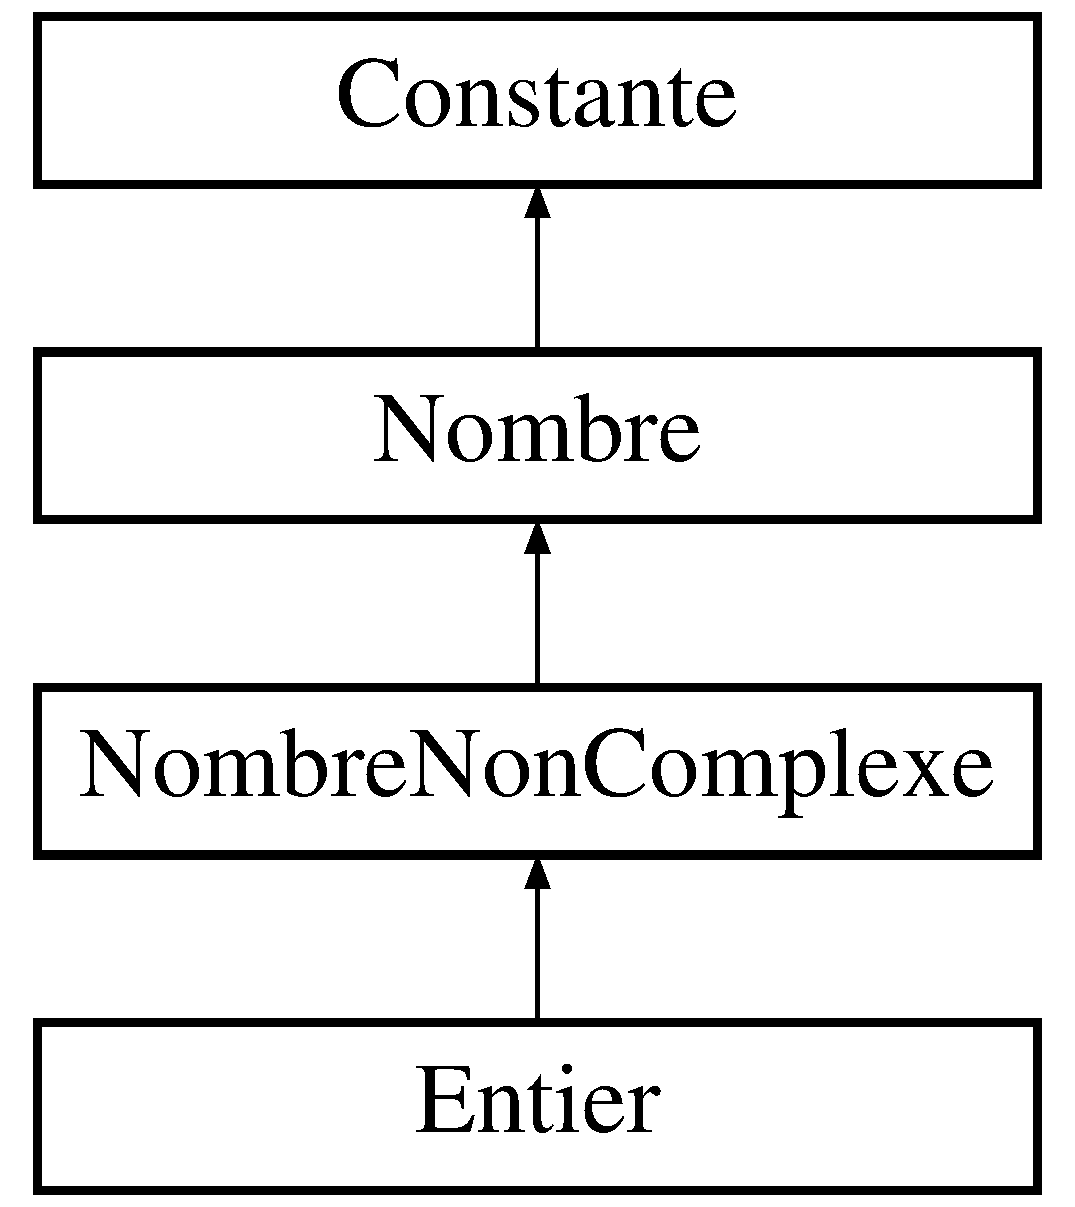
\includegraphics[height=4.000000cm]{class_entier}
\end{center}
\end{figure}
\subsection*{Public Member Functions}
\begin{DoxyCompactItemize}
\item 
\hyperlink{class_entier_a397ae64c08010e930f7d5c7275724f97}{$\sim$\-Entier} ()
\begin{DoxyCompactList}\small\item\em Destructeur de la classe. \end{DoxyCompactList}\item 
\hyperlink{class_entier_a1f0c17b51099803a73a4ec240c5587db}{Entier} ()
\begin{DoxyCompactList}\small\item\em Constructeur par d�faut. \end{DoxyCompactList}\item 
\hyperlink{class_entier_a778672cb4b285a4b69b683f1c27a1340}{Entier} (int v)
\begin{DoxyCompactList}\small\item\em Constructeur avec param�tre. \end{DoxyCompactList}\item 
\hyperlink{class_entier}{Entier} $\ast$ \hyperlink{class_entier_aca1eef6372c8d74274bffd435888ef57}{clone} () const 
\begin{DoxyCompactList}\small\item\em M�thode permettant de cloner une constante.  \end{DoxyCompactList}\item 
\hyperlink{class_entier_a5302773b98799a8d46381a0a7a0e6f01}{Entier} (const \hyperlink{class_entier}{Entier} \&e)
\begin{DoxyCompactList}\small\item\em Cr�e un entier par constructeur par copie. \end{DoxyCompactList}\item 
int \hyperlink{class_entier_ac6b87a29547b9814078220abb1b492fd}{get\-Val} () const 
\begin{DoxyCompactList}\small\item\em Getter de la valeur de l'entier. \end{DoxyCompactList}\item 
void \hyperlink{class_entier_a15a3d4166f1182bd87d0c1ee523d1deb}{fact} ()
\begin{DoxyCompactList}\small\item\em M�thode permettant de transformer le nombre en sa factorielle. \end{DoxyCompactList}\item 
void \hyperlink{class_entier_a0f4e0e38e773c7af216e8aca968f6db6}{mod} (int m)
\begin{DoxyCompactList}\small\item\em M�thode permettant de transformer le nombre en son reste de la division du nombre par m. \end{DoxyCompactList}\item 
void \hyperlink{class_entier_a91748c3918f8eed1c188f5175328cf1a}{sign} ()
\begin{DoxyCompactList}\small\item\em Methode permettant de transformer le nombre en son oppos�.  \end{DoxyCompactList}\item 
void \hyperlink{class_entier_a66dff979b86690f26360fd3a93b25537}{sqr} ()
\begin{DoxyCompactList}\small\item\em M�thode permettant de transformer le nombre en son carr�.  \end{DoxyCompactList}\item 
void \hyperlink{class_entier_a8fbf1379f26622554393e48df17867fd}{cube} ()
\begin{DoxyCompactList}\small\item\em M�thode permettant de transformer le nombre en son cube.  \end{DoxyCompactList}\item 
void \hyperlink{class_entier_ae44b026487bcd10fab16696eff3b49a8}{pow} (\hyperlink{class_entier}{Entier} $\ast$)
\begin{DoxyCompactList}\small\item\em M�thode permettant d'effectuer la puissance d'un nombre.  \end{DoxyCompactList}\item 
Q\-String \hyperlink{class_entier_aa960356dfeae8af6dfa2cd25136a1a6f}{to\-String} () const 
\begin{DoxyCompactList}\small\item\em Fonction permettant de renvoyer une chaine comprenant la valuation de la constante associ�, cette fonction est utilis�e dans le cadre de l'affichage des constantes dans la pile.  \end{DoxyCompactList}\item 
float \hyperlink{class_entier_a4ce7f7cddbaa2a28d244444d18ef55dc}{get\-Float\-Val} () const 
\begin{DoxyCompactList}\small\item\em M�thode permettant de r�cup�rer la valeur du \hyperlink{class_nombre_non_complexe}{Nombre\-Non\-Complexe} sous la forme d'un r�el.  \end{DoxyCompactList}\item 
\hyperlink{class_nombre_complexe}{Nombre\-Complexe} $\ast$ \hyperlink{class_entier_abadca482fe27a3302f874e9e7c109579}{to\-Nombre\-Complexe} ()
\begin{DoxyCompactList}\small\item\em M�thode permettant de convertir un \hyperlink{class_nombre}{Nombre} en son �quivalent en \hyperlink{class_nombre_complexe}{Nombre\-Complexe}.  \end{DoxyCompactList}\end{DoxyCompactItemize}


\subsection{Detailed Description}
Classe impl�mentant l'interface de \hyperlink{class_nombre_non_complexe}{Nombre\-Non\-Complexe} et permettant de g�rer des constantes de type entier. 

Definition at line 20 of file entier.\-h.



\subsection{Constructor \& Destructor Documentation}
\hypertarget{class_entier_a397ae64c08010e930f7d5c7275724f97}{\index{Entier@{Entier}!$\sim$\-Entier@{$\sim$\-Entier}}
\index{$\sim$\-Entier@{$\sim$\-Entier}!Entier@{Entier}}
\subsubsection[{$\sim$\-Entier}]{\setlength{\rightskip}{0pt plus 5cm}{\bf Entier\-::$\sim$\-Entier} (
\begin{DoxyParamCaption}
{}
\end{DoxyParamCaption}
)\hspace{0.3cm}{\ttfamily  \mbox{[}inline\mbox{]}}}}\label{class_entier_a397ae64c08010e930f7d5c7275724f97}


Destructeur de la classe. 



Definition at line 30 of file entier.\-h.

\hypertarget{class_entier_a1f0c17b51099803a73a4ec240c5587db}{\index{Entier@{Entier}!Entier@{Entier}}
\index{Entier@{Entier}!Entier@{Entier}}
\subsubsection[{Entier}]{\setlength{\rightskip}{0pt plus 5cm}{\bf Entier\-::\-Entier} (
\begin{DoxyParamCaption}
{}
\end{DoxyParamCaption}
)\hspace{0.3cm}{\ttfamily  \mbox{[}inline\mbox{]}}}}\label{class_entier_a1f0c17b51099803a73a4ec240c5587db}


Constructeur par d�faut. 



Definition at line 34 of file entier.\-h.

\hypertarget{class_entier_a778672cb4b285a4b69b683f1c27a1340}{\index{Entier@{Entier}!Entier@{Entier}}
\index{Entier@{Entier}!Entier@{Entier}}
\subsubsection[{Entier}]{\setlength{\rightskip}{0pt plus 5cm}{\bf Entier\-::\-Entier} (
\begin{DoxyParamCaption}
\item[{int}]{v}
\end{DoxyParamCaption}
)\hspace{0.3cm}{\ttfamily  \mbox{[}inline\mbox{]}}}}\label{class_entier_a778672cb4b285a4b69b683f1c27a1340}


Constructeur avec param�tre. 


\begin{DoxyParams}{Parameters}
{\em v} & La valeur de l'entier \\
\hline
\end{DoxyParams}


Definition at line 39 of file entier.\-h.

\hypertarget{class_entier_a5302773b98799a8d46381a0a7a0e6f01}{\index{Entier@{Entier}!Entier@{Entier}}
\index{Entier@{Entier}!Entier@{Entier}}
\subsubsection[{Entier}]{\setlength{\rightskip}{0pt plus 5cm}{\bf Entier\-::\-Entier} (
\begin{DoxyParamCaption}
\item[{const {\bf Entier} \&}]{e}
\end{DoxyParamCaption}
)\hspace{0.3cm}{\ttfamily  \mbox{[}inline\mbox{]}}}}\label{class_entier_a5302773b98799a8d46381a0a7a0e6f01}


Cr�e un entier par constructeur par copie. 


\begin{DoxyParams}{Parameters}
{\em e} & L'entier � copier \\
\hline
\end{DoxyParams}


Definition at line 48 of file entier.\-h.



\subsection{Member Function Documentation}
\hypertarget{class_entier_aca1eef6372c8d74274bffd435888ef57}{\index{Entier@{Entier}!clone@{clone}}
\index{clone@{clone}!Entier@{Entier}}
\subsubsection[{clone}]{\setlength{\rightskip}{0pt plus 5cm}{\bf Entier} $\ast$ {\bf Entier\-::clone} (
\begin{DoxyParamCaption}
{}
\end{DoxyParamCaption}
) const\hspace{0.3cm}{\ttfamily  \mbox{[}virtual\mbox{]}}}}\label{class_entier_aca1eef6372c8d74274bffd435888ef57}


M�thode permettant de cloner une constante.  


\begin{DoxyParams}{Parameters}
{\em Le} & pointeur vers la constante clon�e \\
\hline
\end{DoxyParams}
 

Implements \hyperlink{class_constante_a5769ea385161e02bd2d1bcadefc2c510}{Constante}.



Definition at line 10 of file entier.\-cpp.

\hypertarget{class_entier_a8fbf1379f26622554393e48df17867fd}{\index{Entier@{Entier}!cube@{cube}}
\index{cube@{cube}!Entier@{Entier}}
\subsubsection[{cube}]{\setlength{\rightskip}{0pt plus 5cm}void {\bf Entier\-::cube} (
\begin{DoxyParamCaption}
{}
\end{DoxyParamCaption}
)\hspace{0.3cm}{\ttfamily  \mbox{[}inline, virtual\mbox{]}}}}\label{class_entier_a8fbf1379f26622554393e48df17867fd}


M�thode permettant de transformer le nombre en son cube.  



Implements \hyperlink{class_nombre_aed65cb1449858c078e91610afb3a6447}{Nombre}.



Definition at line 74 of file entier.\-h.

\hypertarget{class_entier_a15a3d4166f1182bd87d0c1ee523d1deb}{\index{Entier@{Entier}!fact@{fact}}
\index{fact@{fact}!Entier@{Entier}}
\subsubsection[{fact}]{\setlength{\rightskip}{0pt plus 5cm}void {\bf Entier\-::fact} (
\begin{DoxyParamCaption}
{}
\end{DoxyParamCaption}
)\hspace{0.3cm}{\ttfamily  \mbox{[}inline\mbox{]}}}}\label{class_entier_a15a3d4166f1182bd87d0c1ee523d1deb}


M�thode permettant de transformer le nombre en sa factorielle. 



Definition at line 57 of file entier.\-h.

\hypertarget{class_entier_a4ce7f7cddbaa2a28d244444d18ef55dc}{\index{Entier@{Entier}!get\-Float\-Val@{get\-Float\-Val}}
\index{get\-Float\-Val@{get\-Float\-Val}!Entier@{Entier}}
\subsubsection[{get\-Float\-Val}]{\setlength{\rightskip}{0pt plus 5cm}float {\bf Entier\-::get\-Float\-Val} (
\begin{DoxyParamCaption}
{}
\end{DoxyParamCaption}
) const\hspace{0.3cm}{\ttfamily  \mbox{[}inline, virtual\mbox{]}}}}\label{class_entier_a4ce7f7cddbaa2a28d244444d18ef55dc}


M�thode permettant de r�cup�rer la valeur du \hyperlink{class_nombre_non_complexe}{Nombre\-Non\-Complexe} sous la forme d'un r�el.  

\begin{DoxyReturn}{Returns}
La valeur r�elle 
\end{DoxyReturn}
 

Implements \hyperlink{class_nombre_non_complexe_ad148f1e2a4626ecf279e91d04d1aff24}{Nombre\-Non\-Complexe}.



Definition at line 86 of file entier.\-h.

\hypertarget{class_entier_ac6b87a29547b9814078220abb1b492fd}{\index{Entier@{Entier}!get\-Val@{get\-Val}}
\index{get\-Val@{get\-Val}!Entier@{Entier}}
\subsubsection[{get\-Val}]{\setlength{\rightskip}{0pt plus 5cm}int {\bf Entier\-::get\-Val} (
\begin{DoxyParamCaption}
{}
\end{DoxyParamCaption}
) const\hspace{0.3cm}{\ttfamily  \mbox{[}inline\mbox{]}}}}\label{class_entier_ac6b87a29547b9814078220abb1b492fd}


Getter de la valeur de l'entier. 

\begin{DoxyReturn}{Returns}
La valeur de l'entier 
\end{DoxyReturn}


Definition at line 53 of file entier.\-h.

\hypertarget{class_entier_a0f4e0e38e773c7af216e8aca968f6db6}{\index{Entier@{Entier}!mod@{mod}}
\index{mod@{mod}!Entier@{Entier}}
\subsubsection[{mod}]{\setlength{\rightskip}{0pt plus 5cm}void {\bf Entier\-::mod} (
\begin{DoxyParamCaption}
\item[{int}]{m}
\end{DoxyParamCaption}
)\hspace{0.3cm}{\ttfamily  \mbox{[}inline\mbox{]}}}}\label{class_entier_a0f4e0e38e773c7af216e8aca968f6db6}


M�thode permettant de transformer le nombre en son reste de la division du nombre par m. 


\begin{DoxyParams}{Parameters}
{\em m} & Le diviseur \\
\hline
\end{DoxyParams}


Definition at line 62 of file entier.\-h.

\hypertarget{class_entier_ae44b026487bcd10fab16696eff3b49a8}{\index{Entier@{Entier}!pow@{pow}}
\index{pow@{pow}!Entier@{Entier}}
\subsubsection[{pow}]{\setlength{\rightskip}{0pt plus 5cm}void {\bf Entier\-::pow} (
\begin{DoxyParamCaption}
\item[{{\bf Entier} $\ast$}]{e}
\end{DoxyParamCaption}
)\hspace{0.3cm}{\ttfamily  \mbox{[}virtual\mbox{]}}}}\label{class_entier_ae44b026487bcd10fab16696eff3b49a8}


M�thode permettant d'effectuer la puissance d'un nombre.  


\begin{DoxyParams}{Parameters}
{\em e} & Un entier correspondant � la puissance \\
\hline
\end{DoxyParams}
 

Implements \hyperlink{class_nombre_non_complexe_a859175bae737e01e73316632f1083d07}{Nombre\-Non\-Complexe}.



Definition at line 14 of file entier.\-cpp.

\hypertarget{class_entier_a91748c3918f8eed1c188f5175328cf1a}{\index{Entier@{Entier}!sign@{sign}}
\index{sign@{sign}!Entier@{Entier}}
\subsubsection[{sign}]{\setlength{\rightskip}{0pt plus 5cm}void {\bf Entier\-::sign} (
\begin{DoxyParamCaption}
{}
\end{DoxyParamCaption}
)\hspace{0.3cm}{\ttfamily  \mbox{[}inline, virtual\mbox{]}}}}\label{class_entier_a91748c3918f8eed1c188f5175328cf1a}


Methode permettant de transformer le nombre en son oppos�.  



Implements \hyperlink{class_nombre_a718d616bbf2e5e8f133df958e8bb3d7f}{Nombre}.



Definition at line 66 of file entier.\-h.

\hypertarget{class_entier_a66dff979b86690f26360fd3a93b25537}{\index{Entier@{Entier}!sqr@{sqr}}
\index{sqr@{sqr}!Entier@{Entier}}
\subsubsection[{sqr}]{\setlength{\rightskip}{0pt plus 5cm}void {\bf Entier\-::sqr} (
\begin{DoxyParamCaption}
{}
\end{DoxyParamCaption}
)\hspace{0.3cm}{\ttfamily  \mbox{[}inline, virtual\mbox{]}}}}\label{class_entier_a66dff979b86690f26360fd3a93b25537}


M�thode permettant de transformer le nombre en son carr�.  



Implements \hyperlink{class_nombre_a5be0e66e9bbec508d236ba8dbe1eb6bc}{Nombre}.



Definition at line 70 of file entier.\-h.

\hypertarget{class_entier_abadca482fe27a3302f874e9e7c109579}{\index{Entier@{Entier}!to\-Nombre\-Complexe@{to\-Nombre\-Complexe}}
\index{to\-Nombre\-Complexe@{to\-Nombre\-Complexe}!Entier@{Entier}}
\subsubsection[{to\-Nombre\-Complexe}]{\setlength{\rightskip}{0pt plus 5cm}{\bf Nombre\-Complexe} $\ast$ {\bf Entier\-::to\-Nombre\-Complexe} (
\begin{DoxyParamCaption}
{}
\end{DoxyParamCaption}
)\hspace{0.3cm}{\ttfamily  \mbox{[}virtual\mbox{]}}}}\label{class_entier_abadca482fe27a3302f874e9e7c109579}


M�thode permettant de convertir un \hyperlink{class_nombre}{Nombre} en son �quivalent en \hyperlink{class_nombre_complexe}{Nombre\-Complexe}.  

\begin{DoxyReturn}{Returns}
Le pointeur vers le nombre\-Complexe nouvellement cr�e 
\end{DoxyReturn}
 

Implements \hyperlink{class_nombre_a11092e1fcde81c05b4c518398baf3691}{Nombre}.



Definition at line 6 of file entier.\-cpp.

\hypertarget{class_entier_aa960356dfeae8af6dfa2cd25136a1a6f}{\index{Entier@{Entier}!to\-String@{to\-String}}
\index{to\-String@{to\-String}!Entier@{Entier}}
\subsubsection[{to\-String}]{\setlength{\rightskip}{0pt plus 5cm}Q\-String {\bf Entier\-::to\-String} (
\begin{DoxyParamCaption}
{}
\end{DoxyParamCaption}
) const\hspace{0.3cm}{\ttfamily  \mbox{[}inline, virtual\mbox{]}}}}\label{class_entier_aa960356dfeae8af6dfa2cd25136a1a6f}


Fonction permettant de renvoyer une chaine comprenant la valuation de la constante associ�, cette fonction est utilis�e dans le cadre de l'affichage des constantes dans la pile.  

\begin{DoxyReturn}{Returns}
La chaine � afficher dans la pile 
\end{DoxyReturn}
 

Implements \hyperlink{class_constante_ad5ea6850196ee9f86b74c74009a87ab1}{Constante}.



Definition at line 82 of file entier.\-h.



The documentation for this class was generated from the following files\-:\begin{DoxyCompactItemize}
\item 
\hyperlink{entier_8h}{entier.\-h}\item 
\hyperlink{entier_8cpp}{entier.\-cpp}\end{DoxyCompactItemize}

\hypertarget{class_expression}{\section{Expression Class Reference}
\label{class_expression}\index{Expression@{Expression}}
}


Classe impl�mentant l'interface de \hyperlink{class_constante}{Constante} et permettant la gestion d'un expression.  




{\ttfamily \#include $<$expression.\-h$>$}

Inheritance diagram for Expression\-:\begin{figure}[H]
\begin{center}
\leavevmode
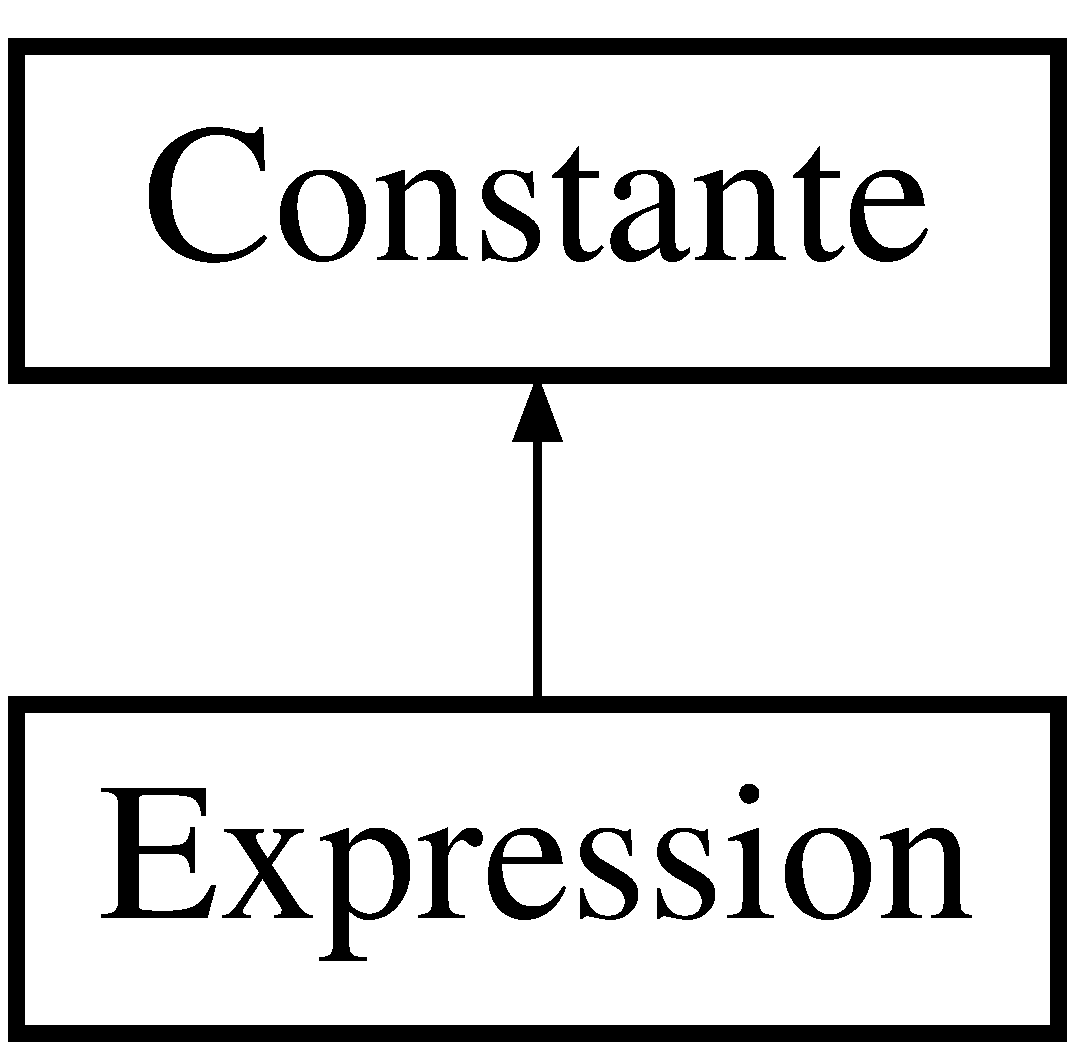
\includegraphics[height=2.000000cm]{class_expression}
\end{center}
\end{figure}
\subsection*{Public Member Functions}
\begin{DoxyCompactItemize}
\item 
\hyperlink{class_expression_afcf87716bf0abfe8d414c92529e1564a}{Expression} ()
\begin{DoxyCompactList}\small\item\em Constructeur par d�faut. \end{DoxyCompactList}\item 
\hyperlink{class_expression_aeefdef970387f310f7b84c840045f51e}{Expression} (const Q\-String \&str)
\begin{DoxyCompactList}\small\item\em Constructeur par copie. \end{DoxyCompactList}\item 
\hyperlink{class_expression}{Expression} $\ast$ \hyperlink{class_expression_ad357e8bb1174b3582833ebcbf6d6e232}{clone} () const 
\begin{DoxyCompactList}\small\item\em M�thode permettant de cloner une constante.  \end{DoxyCompactList}\item 
Q\-String \hyperlink{class_expression_ae1a9e65c034a2614977955cf5bfc8b05}{get\-Liste} () const 
\begin{DoxyCompactList}\small\item\em M�thode permettant de retourner la chaine contenant l'expression. \end{DoxyCompactList}\item 
void \hyperlink{class_expression_a6828fe53c893fa3b8c8357bc2c9482f9}{set\-Liste} (const Q\-String \&str)
\begin{DoxyCompactList}\small\item\em M�thode permettant de modifier la chaine contenant l'expression. \end{DoxyCompactList}\item 
Q\-String \hyperlink{class_expression_a60e6e305cdd8e878df2e3081ae15a4d0}{to\-String} () const 
\begin{DoxyCompactList}\small\item\em Fonction permettant de renvoyer une chaine comprenant la valuation de la constante associ�, cette fonction est utilis�e dans le cadre de l'affichage des constantes dans la pile.  \end{DoxyCompactList}\item 
\hyperlink{class_expression}{Expression} $\ast$ \hyperlink{class_expression_a14c9ec2a29777e43b07447cfcdbf5968}{operator+} (\hyperlink{class_constante}{Constante} $\ast$c)
\begin{DoxyCompactList}\small\item\em M�thode permettant de retourner une expression contenant l'expression appelante, la constante pass�e en param�tre et ainsi que l'op�rateur associ� ('+'). \end{DoxyCompactList}\item 
\hyperlink{class_expression}{Expression} $\ast$ \hyperlink{class_expression_ab0f151eea8c2920a41d9b88b835ffbac}{operator-\/} (\hyperlink{class_constante}{Constante} $\ast$c)
\begin{DoxyCompactList}\small\item\em M�thode permettant de retourner une expression contenant l'expression appelante, la constante pass�e en param�tre et ainsi que l'op�rateur associ� ('-\/'). \end{DoxyCompactList}\item 
\hyperlink{class_expression}{Expression} $\ast$ \hyperlink{class_expression_a4117f2eff2bb19a7d9b96696d97a0be7}{operator$\ast$} (\hyperlink{class_constante}{Constante} $\ast$c)
\begin{DoxyCompactList}\small\item\em M�thode permettant de retourner une expression contenant l'expression appelante, la constante pass�e en param�tre et ainsi que l'op�rateur associ� ('$\ast$'). \end{DoxyCompactList}\item 
\hyperlink{class_expression}{Expression} $\ast$ \hyperlink{class_expression_ae3924fe2659a6c1b465a14d24296498c}{operator/} (\hyperlink{class_constante}{Constante} $\ast$c)
\begin{DoxyCompactList}\small\item\em M�thode permettant de retourner une expression contenant l'expression appelante, la constante pass�e en param�tre et ainsi que l'op�rateur associ� ('/'). \end{DoxyCompactList}\end{DoxyCompactItemize}


\subsection{Detailed Description}
Classe impl�mentant l'interface de \hyperlink{class_constante}{Constante} et permettant la gestion d'un expression. 

Definition at line 19 of file expression.\-h.



\subsection{Constructor \& Destructor Documentation}
\hypertarget{class_expression_afcf87716bf0abfe8d414c92529e1564a}{\index{Expression@{Expression}!Expression@{Expression}}
\index{Expression@{Expression}!Expression@{Expression}}
\subsubsection[{Expression}]{\setlength{\rightskip}{0pt plus 5cm}{\bf Expression\-::\-Expression} (
\begin{DoxyParamCaption}
{}
\end{DoxyParamCaption}
)}}\label{class_expression_afcf87716bf0abfe8d414c92529e1564a}


Constructeur par d�faut. 



Definition at line 5 of file expression.\-cpp.

\hypertarget{class_expression_aeefdef970387f310f7b84c840045f51e}{\index{Expression@{Expression}!Expression@{Expression}}
\index{Expression@{Expression}!Expression@{Expression}}
\subsubsection[{Expression}]{\setlength{\rightskip}{0pt plus 5cm}{\bf Expression\-::\-Expression} (
\begin{DoxyParamCaption}
\item[{const Q\-String \&}]{str}
\end{DoxyParamCaption}
)}}\label{class_expression_aeefdef970387f310f7b84c840045f51e}


Constructeur par copie. 



Definition at line 8 of file expression.\-cpp.



\subsection{Member Function Documentation}
\hypertarget{class_expression_ad357e8bb1174b3582833ebcbf6d6e232}{\index{Expression@{Expression}!clone@{clone}}
\index{clone@{clone}!Expression@{Expression}}
\subsubsection[{clone}]{\setlength{\rightskip}{0pt plus 5cm}{\bf Expression} $\ast$ {\bf Expression\-::clone} (
\begin{DoxyParamCaption}
{}
\end{DoxyParamCaption}
) const\hspace{0.3cm}{\ttfamily  \mbox{[}virtual\mbox{]}}}}\label{class_expression_ad357e8bb1174b3582833ebcbf6d6e232}


M�thode permettant de cloner une constante.  


\begin{DoxyParams}{Parameters}
{\em Le} & pointeur vers la constante clon�e \\
\hline
\end{DoxyParams}
 

Implements \hyperlink{class_constante_a5769ea385161e02bd2d1bcadefc2c510}{Constante}.



Definition at line 12 of file expression.\-cpp.

\hypertarget{class_expression_ae1a9e65c034a2614977955cf5bfc8b05}{\index{Expression@{Expression}!get\-Liste@{get\-Liste}}
\index{get\-Liste@{get\-Liste}!Expression@{Expression}}
\subsubsection[{get\-Liste}]{\setlength{\rightskip}{0pt plus 5cm}Q\-String {\bf Expression\-::get\-Liste} (
\begin{DoxyParamCaption}
{}
\end{DoxyParamCaption}
) const\hspace{0.3cm}{\ttfamily  \mbox{[}inline\mbox{]}}}}\label{class_expression_ae1a9e65c034a2614977955cf5bfc8b05}


M�thode permettant de retourner la chaine contenant l'expression. 

\begin{DoxyReturn}{Returns}
La chaine de l'expression 
\end{DoxyReturn}


Definition at line 42 of file expression.\-h.

\hypertarget{class_expression_a4117f2eff2bb19a7d9b96696d97a0be7}{\index{Expression@{Expression}!operator$\ast$@{operator$\ast$}}
\index{operator$\ast$@{operator$\ast$}!Expression@{Expression}}
\subsubsection[{operator$\ast$}]{\setlength{\rightskip}{0pt plus 5cm}{\bf Expression} $\ast$ Expression\-::operator$\ast$ (
\begin{DoxyParamCaption}
\item[{{\bf Constante} $\ast$}]{c}
\end{DoxyParamCaption}
)}}\label{class_expression_a4117f2eff2bb19a7d9b96696d97a0be7}


M�thode permettant de retourner une expression contenant l'expression appelante, la constante pass�e en param�tre et ainsi que l'op�rateur associ� ('$\ast$'). 


\begin{DoxyParams}{Parameters}
{\em c} & La constante � ins�rer dans l'expression \\
\hline
\end{DoxyParams}
\begin{DoxyReturn}{Returns}
L'expression ressortissante de l'op�ration 
\end{DoxyReturn}


Definition at line 50 of file expression.\-cpp.

\hypertarget{class_expression_a14c9ec2a29777e43b07447cfcdbf5968}{\index{Expression@{Expression}!operator+@{operator+}}
\index{operator+@{operator+}!Expression@{Expression}}
\subsubsection[{operator+}]{\setlength{\rightskip}{0pt plus 5cm}{\bf Expression} $\ast$ Expression\-::operator+ (
\begin{DoxyParamCaption}
\item[{{\bf Constante} $\ast$}]{c}
\end{DoxyParamCaption}
)}}\label{class_expression_a14c9ec2a29777e43b07447cfcdbf5968}


M�thode permettant de retourner une expression contenant l'expression appelante, la constante pass�e en param�tre et ainsi que l'op�rateur associ� ('+'). 


\begin{DoxyParams}{Parameters}
{\em c} & La constante � ins�rer dans l'expression \\
\hline
\end{DoxyParams}
\begin{DoxyReturn}{Returns}
L'expression ressortissante de l'op�ration 
\end{DoxyReturn}


Definition at line 24 of file expression.\-cpp.

\hypertarget{class_expression_ab0f151eea8c2920a41d9b88b835ffbac}{\index{Expression@{Expression}!operator-\/@{operator-\/}}
\index{operator-\/@{operator-\/}!Expression@{Expression}}
\subsubsection[{operator-\/}]{\setlength{\rightskip}{0pt plus 5cm}{\bf Expression} $\ast$ Expression\-::operator-\/ (
\begin{DoxyParamCaption}
\item[{{\bf Constante} $\ast$}]{c}
\end{DoxyParamCaption}
)}}\label{class_expression_ab0f151eea8c2920a41d9b88b835ffbac}


M�thode permettant de retourner une expression contenant l'expression appelante, la constante pass�e en param�tre et ainsi que l'op�rateur associ� ('-\/'). 


\begin{DoxyParams}{Parameters}
{\em c} & La constante � ins�rer dans l'expression \\
\hline
\end{DoxyParams}
\begin{DoxyReturn}{Returns}
L'expression ressortissante de l'op�ration 
\end{DoxyReturn}


Definition at line 39 of file expression.\-cpp.

\hypertarget{class_expression_ae3924fe2659a6c1b465a14d24296498c}{\index{Expression@{Expression}!operator/@{operator/}}
\index{operator/@{operator/}!Expression@{Expression}}
\subsubsection[{operator/}]{\setlength{\rightskip}{0pt plus 5cm}{\bf Expression} $\ast$ Expression\-::operator/ (
\begin{DoxyParamCaption}
\item[{{\bf Constante} $\ast$}]{c}
\end{DoxyParamCaption}
)}}\label{class_expression_ae3924fe2659a6c1b465a14d24296498c}


M�thode permettant de retourner une expression contenant l'expression appelante, la constante pass�e en param�tre et ainsi que l'op�rateur associ� ('/'). 


\begin{DoxyParams}{Parameters}
{\em c} & La constante � ins�rer dans l'expression \\
\hline
\end{DoxyParams}
\begin{DoxyReturn}{Returns}
L'expression ressortissante de l'op�ration 
\end{DoxyReturn}


Definition at line 61 of file expression.\-cpp.

\hypertarget{class_expression_a6828fe53c893fa3b8c8357bc2c9482f9}{\index{Expression@{Expression}!set\-Liste@{set\-Liste}}
\index{set\-Liste@{set\-Liste}!Expression@{Expression}}
\subsubsection[{set\-Liste}]{\setlength{\rightskip}{0pt plus 5cm}void {\bf Expression\-::set\-Liste} (
\begin{DoxyParamCaption}
\item[{const Q\-String \&}]{str}
\end{DoxyParamCaption}
)\hspace{0.3cm}{\ttfamily  \mbox{[}inline\mbox{]}}}}\label{class_expression_a6828fe53c893fa3b8c8357bc2c9482f9}


M�thode permettant de modifier la chaine contenant l'expression. 


\begin{DoxyParams}{Parameters}
{\em La} & nouvelle chaine de l'expression \\
\hline
\end{DoxyParams}


Definition at line 47 of file expression.\-h.

\hypertarget{class_expression_a60e6e305cdd8e878df2e3081ae15a4d0}{\index{Expression@{Expression}!to\-String@{to\-String}}
\index{to\-String@{to\-String}!Expression@{Expression}}
\subsubsection[{to\-String}]{\setlength{\rightskip}{0pt plus 5cm}Q\-String {\bf Expression\-::to\-String} (
\begin{DoxyParamCaption}
{}
\end{DoxyParamCaption}
) const\hspace{0.3cm}{\ttfamily  \mbox{[}virtual\mbox{]}}}}\label{class_expression_a60e6e305cdd8e878df2e3081ae15a4d0}


Fonction permettant de renvoyer une chaine comprenant la valuation de la constante associ�, cette fonction est utilis�e dans le cadre de l'affichage des constantes dans la pile.  

\begin{DoxyReturn}{Returns}
La chaine � afficher dans la pile 
\end{DoxyReturn}
 

Implements \hyperlink{class_constante_ad5ea6850196ee9f86b74c74009a87ab1}{Constante}.



Definition at line 16 of file expression.\-cpp.



The documentation for this class was generated from the following files\-:\begin{DoxyCompactItemize}
\item 
\hyperlink{expression_8h}{expression.\-h}\item 
\hyperlink{expression_8cpp}{expression.\-cpp}\end{DoxyCompactItemize}

\hypertarget{class_historique}{\section{Historique Class Reference}
\label{class_historique}\index{Historique@{Historique}}
}


Classe (utilisant le design pattern command) abstraite permettant de g�rer des objets de type \hyperlink{class_historique}{Historique}.  




{\ttfamily \#include $<$historique.\-h$>$}

Inheritance diagram for Historique\-:\begin{figure}[H]
\begin{center}
\leavevmode
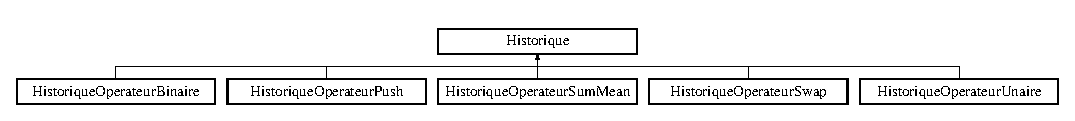
\includegraphics[height=1.178947cm]{class_historique}
\end{center}
\end{figure}
\subsection*{Public Member Functions}
\begin{DoxyCompactItemize}
\item 
virtual void \hyperlink{class_historique_ac0247bb67a9535851abe5f76113b4751}{undo} ()=0
\begin{DoxyCompactList}\small\item\em M�thode virtuelle pure permettant d'effectuer un \char`\"{}undo\char`\"{} sur la commande courante. \end{DoxyCompactList}\item 
virtual void \hyperlink{class_historique_ad9d996361bf9a68280d8c558da1cd182}{redo} ()=0
\begin{DoxyCompactList}\small\item\em M�thode virtuelle pure permettant d'effectuer un \char`\"{}redo\char`\"{} sur la commande courante. \end{DoxyCompactList}\end{DoxyCompactItemize}


\subsection{Detailed Description}
Classe (utilisant le design pattern command) abstraite permettant de g�rer des objets de type \hyperlink{class_historique}{Historique}. 

Definition at line 15 of file historique.\-h.



\subsection{Member Function Documentation}
\hypertarget{class_historique_ad9d996361bf9a68280d8c558da1cd182}{\index{Historique@{Historique}!redo@{redo}}
\index{redo@{redo}!Historique@{Historique}}
\subsubsection[{redo}]{\setlength{\rightskip}{0pt plus 5cm}virtual void {\bf Historique\-::redo} (
\begin{DoxyParamCaption}
{}
\end{DoxyParamCaption}
)\hspace{0.3cm}{\ttfamily  \mbox{[}pure virtual\mbox{]}}}}\label{class_historique_ad9d996361bf9a68280d8c558da1cd182}


M�thode virtuelle pure permettant d'effectuer un \char`\"{}redo\char`\"{} sur la commande courante. 



Implemented in \hyperlink{class_historique_operateur_binaire_a31568768a3917965d205ef7da3d01d9c}{Historique\-Operateur\-Binaire}, \hyperlink{class_historique_operateur_sum_mean_a9b6b410f0e49877768d84adfd76da76c}{Historique\-Operateur\-Sum\-Mean}, \hyperlink{class_historique_operateur_unaire_a57f9d18a4a6ece2a9bb4797003c6f6bc}{Historique\-Operateur\-Unaire}, \hyperlink{class_historique_operateur_swap_a48aaa552de5396f614974709b5a61e99}{Historique\-Operateur\-Swap}, and \hyperlink{class_historique_operateur_push_a7107fd5ca184d15928c4cdb3afc6aa06}{Historique\-Operateur\-Push}.

\hypertarget{class_historique_ac0247bb67a9535851abe5f76113b4751}{\index{Historique@{Historique}!undo@{undo}}
\index{undo@{undo}!Historique@{Historique}}
\subsubsection[{undo}]{\setlength{\rightskip}{0pt plus 5cm}virtual void {\bf Historique\-::undo} (
\begin{DoxyParamCaption}
{}
\end{DoxyParamCaption}
)\hspace{0.3cm}{\ttfamily  \mbox{[}pure virtual\mbox{]}}}}\label{class_historique_ac0247bb67a9535851abe5f76113b4751}


M�thode virtuelle pure permettant d'effectuer un \char`\"{}undo\char`\"{} sur la commande courante. 



Implemented in \hyperlink{class_historique_operateur_binaire_a5ac8414021420980cf41f69ab3d0ae0c}{Historique\-Operateur\-Binaire}, \hyperlink{class_historique_operateur_sum_mean_a5fe3719f36bea1738a0de3ede63f2bf6}{Historique\-Operateur\-Sum\-Mean}, \hyperlink{class_historique_operateur_unaire_aebd86086fd2ce41cd529035a8140c262}{Historique\-Operateur\-Unaire}, \hyperlink{class_historique_operateur_swap_a71cad4d42084faee7a61f21fe93178be}{Historique\-Operateur\-Swap}, and \hyperlink{class_historique_operateur_push_ac6ad8c7ae0ebd81713ae1e6d1feb7c44}{Historique\-Operateur\-Push}.



The documentation for this class was generated from the following file\-:\begin{DoxyCompactItemize}
\item 
\hyperlink{historique_8h}{historique.\-h}\end{DoxyCompactItemize}

\hypertarget{class_historique_operateur_binaire}{\section{Historique\-Operateur\-Binaire Class Reference}
\label{class_historique_operateur_binaire}\index{Historique\-Operateur\-Binaire@{Historique\-Operateur\-Binaire}}
}


Classe impl�mentant l'interface \hyperlink{class_historique}{Historique} et permettant de g�rer l'historique de toute les commandes binaires.  




{\ttfamily \#include $<$historique\-Operateur\-Binaire.\-h$>$}

Inheritance diagram for Historique\-Operateur\-Binaire\-:\begin{figure}[H]
\begin{center}
\leavevmode
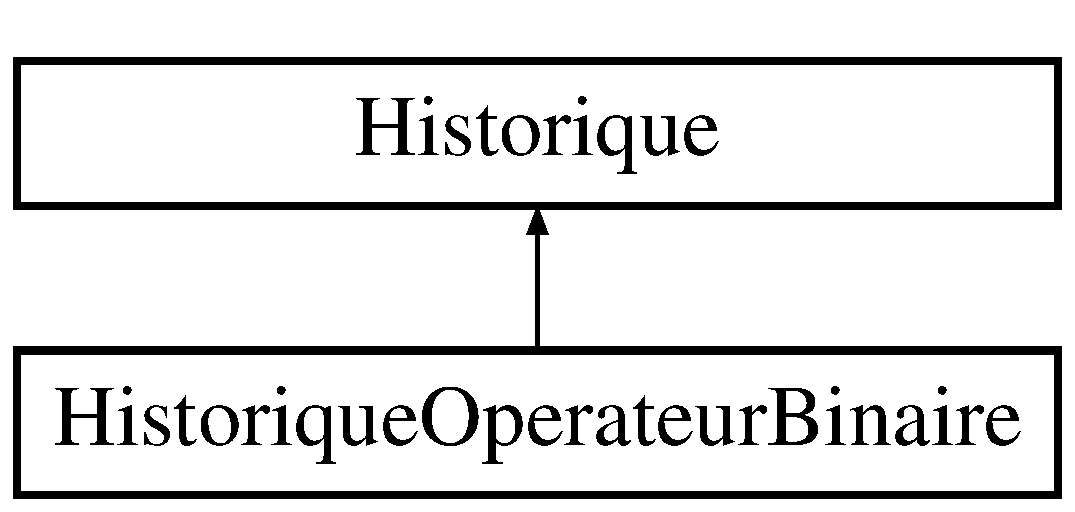
\includegraphics[height=2.000000cm]{class_historique_operateur_binaire}
\end{center}
\end{figure}
\subsection*{Public Member Functions}
\begin{DoxyCompactItemize}
\item 
\hyperlink{class_historique_operateur_binaire_a547071f22bad19ad473c5a7c8d16cc5f}{Historique\-Operateur\-Binaire} (\hyperlink{class_constante}{Constante} $\ast$c1, \hyperlink{class_constante}{Constante} $\ast$c2)
\begin{DoxyCompactList}\small\item\em Constructeur avec parametres. \end{DoxyCompactList}\item 
\hyperlink{class_historique_operateur_binaire_a233825f39453cb95ae94a0bfed43f1d8}{$\sim$\-Historique\-Operateur\-Binaire} ()
\begin{DoxyCompactList}\small\item\em Destructeur de la classe. \end{DoxyCompactList}\item 
\hyperlink{class_constante}{Constante} $\ast$ \hyperlink{class_historique_operateur_binaire_ae8739b2a5c70e438233776b7fff5de14}{set\-Resultat} (\hyperlink{class_constante}{Constante} $\ast$res)
\begin{DoxyCompactList}\small\item\em M�thode permettant de stocker le r�sultat de la commande dans l'attribut \-\_\-resultat de la classe. \end{DoxyCompactList}\item 
void \hyperlink{class_historique_operateur_binaire_a5ac8414021420980cf41f69ab3d0ae0c}{undo} ()
\begin{DoxyCompactList}\small\item\em M�thode virtuelle pure permettant d'effectuer un \char`\"{}undo\char`\"{} sur la commande courante.  \end{DoxyCompactList}\item 
void \hyperlink{class_historique_operateur_binaire_a31568768a3917965d205ef7da3d01d9c}{redo} ()
\begin{DoxyCompactList}\small\item\em M�thode virtuelle pure permettant d'effectuer un \char`\"{}redo\char`\"{} sur la commande courante.  \end{DoxyCompactList}\end{DoxyCompactItemize}


\subsection{Detailed Description}
Classe impl�mentant l'interface \hyperlink{class_historique}{Historique} et permettant de g�rer l'historique de toute les commandes binaires. 

Definition at line 18 of file historique\-Operateur\-Binaire.\-h.



\subsection{Constructor \& Destructor Documentation}
\hypertarget{class_historique_operateur_binaire_a547071f22bad19ad473c5a7c8d16cc5f}{\index{Historique\-Operateur\-Binaire@{Historique\-Operateur\-Binaire}!Historique\-Operateur\-Binaire@{Historique\-Operateur\-Binaire}}
\index{Historique\-Operateur\-Binaire@{Historique\-Operateur\-Binaire}!HistoriqueOperateurBinaire@{Historique\-Operateur\-Binaire}}
\subsubsection[{Historique\-Operateur\-Binaire}]{\setlength{\rightskip}{0pt plus 5cm}{\bf Historique\-Operateur\-Binaire\-::\-Historique\-Operateur\-Binaire} (
\begin{DoxyParamCaption}
\item[{{\bf Constante} $\ast$}]{c1, }
\item[{{\bf Constante} $\ast$}]{c2}
\end{DoxyParamCaption}
)\hspace{0.3cm}{\ttfamily  \mbox{[}inline\mbox{]}}}}\label{class_historique_operateur_binaire_a547071f22bad19ad473c5a7c8d16cc5f}


Constructeur avec parametres. 


\begin{DoxyParams}{Parameters}
{\em c1} & La premi�re op�rande de la commande \\
\hline
{\em c2} & La seconde op�rande de la commande \\
\hline
\end{DoxyParams}


Definition at line 37 of file historique\-Operateur\-Binaire.\-h.

\hypertarget{class_historique_operateur_binaire_a233825f39453cb95ae94a0bfed43f1d8}{\index{Historique\-Operateur\-Binaire@{Historique\-Operateur\-Binaire}!$\sim$\-Historique\-Operateur\-Binaire@{$\sim$\-Historique\-Operateur\-Binaire}}
\index{$\sim$\-Historique\-Operateur\-Binaire@{$\sim$\-Historique\-Operateur\-Binaire}!HistoriqueOperateurBinaire@{Historique\-Operateur\-Binaire}}
\subsubsection[{$\sim$\-Historique\-Operateur\-Binaire}]{\setlength{\rightskip}{0pt plus 5cm}{\bf Historique\-Operateur\-Binaire\-::$\sim$\-Historique\-Operateur\-Binaire} (
\begin{DoxyParamCaption}
{}
\end{DoxyParamCaption}
)\hspace{0.3cm}{\ttfamily  \mbox{[}inline\mbox{]}}}}\label{class_historique_operateur_binaire_a233825f39453cb95ae94a0bfed43f1d8}


Destructeur de la classe. 



Definition at line 41 of file historique\-Operateur\-Binaire.\-h.



\subsection{Member Function Documentation}
\hypertarget{class_historique_operateur_binaire_a31568768a3917965d205ef7da3d01d9c}{\index{Historique\-Operateur\-Binaire@{Historique\-Operateur\-Binaire}!redo@{redo}}
\index{redo@{redo}!HistoriqueOperateurBinaire@{Historique\-Operateur\-Binaire}}
\subsubsection[{redo}]{\setlength{\rightskip}{0pt plus 5cm}void {\bf Historique\-Operateur\-Binaire\-::redo} (
\begin{DoxyParamCaption}
{}
\end{DoxyParamCaption}
)\hspace{0.3cm}{\ttfamily  \mbox{[}virtual\mbox{]}}}}\label{class_historique_operateur_binaire_a31568768a3917965d205ef7da3d01d9c}


M�thode virtuelle pure permettant d'effectuer un \char`\"{}redo\char`\"{} sur la commande courante.  



Implements \hyperlink{class_historique_ad9d996361bf9a68280d8c558da1cd182}{Historique}.



Definition at line 10 of file historique\-Operateur\-Binaire.\-cpp.

\hypertarget{class_historique_operateur_binaire_ae8739b2a5c70e438233776b7fff5de14}{\index{Historique\-Operateur\-Binaire@{Historique\-Operateur\-Binaire}!set\-Resultat@{set\-Resultat}}
\index{set\-Resultat@{set\-Resultat}!HistoriqueOperateurBinaire@{Historique\-Operateur\-Binaire}}
\subsubsection[{set\-Resultat}]{\setlength{\rightskip}{0pt plus 5cm}{\bf Constante}$\ast$ {\bf Historique\-Operateur\-Binaire\-::set\-Resultat} (
\begin{DoxyParamCaption}
\item[{{\bf Constante} $\ast$}]{res}
\end{DoxyParamCaption}
)\hspace{0.3cm}{\ttfamily  \mbox{[}inline\mbox{]}}}}\label{class_historique_operateur_binaire_ae8739b2a5c70e438233776b7fff5de14}


M�thode permettant de stocker le r�sultat de la commande dans l'attribut \-\_\-resultat de la classe. 


\begin{DoxyParams}{Parameters}
{\em res} & Le r�sultat de l'op�ration \\
\hline
\end{DoxyParams}
\begin{DoxyReturn}{Returns}
Le r�sultat de l'op�ration 
\end{DoxyReturn}


Definition at line 47 of file historique\-Operateur\-Binaire.\-h.

\hypertarget{class_historique_operateur_binaire_a5ac8414021420980cf41f69ab3d0ae0c}{\index{Historique\-Operateur\-Binaire@{Historique\-Operateur\-Binaire}!undo@{undo}}
\index{undo@{undo}!HistoriqueOperateurBinaire@{Historique\-Operateur\-Binaire}}
\subsubsection[{undo}]{\setlength{\rightskip}{0pt plus 5cm}void {\bf Historique\-Operateur\-Binaire\-::undo} (
\begin{DoxyParamCaption}
{}
\end{DoxyParamCaption}
)\hspace{0.3cm}{\ttfamily  \mbox{[}virtual\mbox{]}}}}\label{class_historique_operateur_binaire_a5ac8414021420980cf41f69ab3d0ae0c}


M�thode virtuelle pure permettant d'effectuer un \char`\"{}undo\char`\"{} sur la commande courante.  



Implements \hyperlink{class_historique_ac0247bb67a9535851abe5f76113b4751}{Historique}.



Definition at line 4 of file historique\-Operateur\-Binaire.\-cpp.



The documentation for this class was generated from the following files\-:\begin{DoxyCompactItemize}
\item 
\hyperlink{historique_operateur_binaire_8h}{historique\-Operateur\-Binaire.\-h}\item 
\hyperlink{historique_operateur_binaire_8cpp}{historique\-Operateur\-Binaire.\-cpp}\end{DoxyCompactItemize}

\hypertarget{class_historique_operateur_push}{\section{Historique\-Operateur\-Push Class Reference}
\label{class_historique_operateur_push}\index{Historique\-Operateur\-Push@{Historique\-Operateur\-Push}}
}


Classe impl�mentant l'interface \hyperlink{class_historique}{Historique} et permettant de g�rer l'historique de tous les push.  




{\ttfamily \#include $<$historique\-Operateur\-Push.\-h$>$}

Inheritance diagram for Historique\-Operateur\-Push\-:\begin{figure}[H]
\begin{center}
\leavevmode
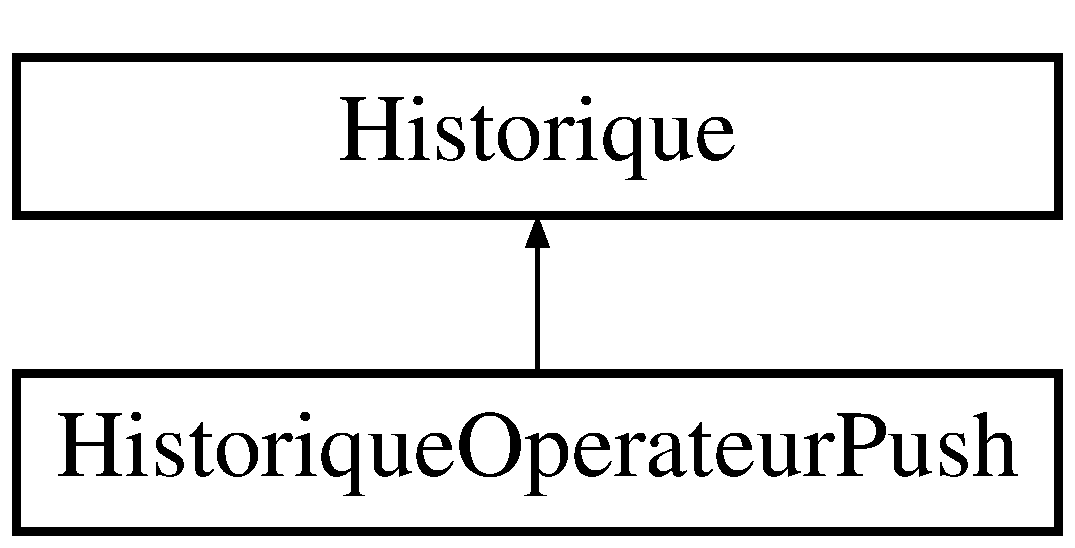
\includegraphics[height=2.000000cm]{class_historique_operateur_push}
\end{center}
\end{figure}
\subsection*{Public Member Functions}
\begin{DoxyCompactItemize}
\item 
\hyperlink{class_historique_operateur_push_a42b86c881529cde894a4e2869b3f7dc4}{Historique\-Operateur\-Push} (\hyperlink{class_constante}{Constante} $\ast$c1)
\begin{DoxyCompactList}\small\item\em Constructeur avec param�tre. \end{DoxyCompactList}\item 
\hyperlink{class_historique_operateur_push_ab58cc5dccc938a4f8431096b7f908e7c}{$\sim$\-Historique\-Operateur\-Push} ()
\begin{DoxyCompactList}\small\item\em Destructeur de la classe. \end{DoxyCompactList}\item 
void \hyperlink{class_historique_operateur_push_ac6ad8c7ae0ebd81713ae1e6d1feb7c44}{undo} ()
\begin{DoxyCompactList}\small\item\em M�thode virtuelle pure permettant d'effectuer un \char`\"{}undo\char`\"{} sur la commande courante.  \end{DoxyCompactList}\item 
void \hyperlink{class_historique_operateur_push_a7107fd5ca184d15928c4cdb3afc6aa06}{redo} ()
\begin{DoxyCompactList}\small\item\em M�thode virtuelle pure permettant d'effectuer un \char`\"{}redo\char`\"{} sur la commande courante.  \end{DoxyCompactList}\end{DoxyCompactItemize}


\subsection{Detailed Description}
Classe impl�mentant l'interface \hyperlink{class_historique}{Historique} et permettant de g�rer l'historique de tous les push. 

Definition at line 18 of file historique\-Operateur\-Push.\-h.



\subsection{Constructor \& Destructor Documentation}
\hypertarget{class_historique_operateur_push_a42b86c881529cde894a4e2869b3f7dc4}{\index{Historique\-Operateur\-Push@{Historique\-Operateur\-Push}!Historique\-Operateur\-Push@{Historique\-Operateur\-Push}}
\index{Historique\-Operateur\-Push@{Historique\-Operateur\-Push}!HistoriqueOperateurPush@{Historique\-Operateur\-Push}}
\subsubsection[{Historique\-Operateur\-Push}]{\setlength{\rightskip}{0pt plus 5cm}{\bf Historique\-Operateur\-Push\-::\-Historique\-Operateur\-Push} (
\begin{DoxyParamCaption}
\item[{{\bf Constante} $\ast$}]{c1}
\end{DoxyParamCaption}
)\hspace{0.3cm}{\ttfamily  \mbox{[}inline\mbox{]}}}}\label{class_historique_operateur_push_a42b86c881529cde894a4e2869b3f7dc4}


Constructeur avec param�tre. 


\begin{DoxyParams}{Parameters}
{\em c1} & La constante qui est ins�r�e au cours d'un push \\
\hline
\end{DoxyParams}


Definition at line 28 of file historique\-Operateur\-Push.\-h.

\hypertarget{class_historique_operateur_push_ab58cc5dccc938a4f8431096b7f908e7c}{\index{Historique\-Operateur\-Push@{Historique\-Operateur\-Push}!$\sim$\-Historique\-Operateur\-Push@{$\sim$\-Historique\-Operateur\-Push}}
\index{$\sim$\-Historique\-Operateur\-Push@{$\sim$\-Historique\-Operateur\-Push}!HistoriqueOperateurPush@{Historique\-Operateur\-Push}}
\subsubsection[{$\sim$\-Historique\-Operateur\-Push}]{\setlength{\rightskip}{0pt plus 5cm}{\bf Historique\-Operateur\-Push\-::$\sim$\-Historique\-Operateur\-Push} (
\begin{DoxyParamCaption}
{}
\end{DoxyParamCaption}
)\hspace{0.3cm}{\ttfamily  \mbox{[}inline\mbox{]}}}}\label{class_historique_operateur_push_ab58cc5dccc938a4f8431096b7f908e7c}


Destructeur de la classe. 



Definition at line 32 of file historique\-Operateur\-Push.\-h.



\subsection{Member Function Documentation}
\hypertarget{class_historique_operateur_push_a7107fd5ca184d15928c4cdb3afc6aa06}{\index{Historique\-Operateur\-Push@{Historique\-Operateur\-Push}!redo@{redo}}
\index{redo@{redo}!HistoriqueOperateurPush@{Historique\-Operateur\-Push}}
\subsubsection[{redo}]{\setlength{\rightskip}{0pt plus 5cm}void {\bf Historique\-Operateur\-Push\-::redo} (
\begin{DoxyParamCaption}
{}
\end{DoxyParamCaption}
)\hspace{0.3cm}{\ttfamily  \mbox{[}virtual\mbox{]}}}}\label{class_historique_operateur_push_a7107fd5ca184d15928c4cdb3afc6aa06}


M�thode virtuelle pure permettant d'effectuer un \char`\"{}redo\char`\"{} sur la commande courante.  



Implements \hyperlink{class_historique_ad9d996361bf9a68280d8c558da1cd182}{Historique}.



Definition at line 8 of file historique\-Operateur\-Push.\-cpp.

\hypertarget{class_historique_operateur_push_ac6ad8c7ae0ebd81713ae1e6d1feb7c44}{\index{Historique\-Operateur\-Push@{Historique\-Operateur\-Push}!undo@{undo}}
\index{undo@{undo}!HistoriqueOperateurPush@{Historique\-Operateur\-Push}}
\subsubsection[{undo}]{\setlength{\rightskip}{0pt plus 5cm}void {\bf Historique\-Operateur\-Push\-::undo} (
\begin{DoxyParamCaption}
{}
\end{DoxyParamCaption}
)\hspace{0.3cm}{\ttfamily  \mbox{[}virtual\mbox{]}}}}\label{class_historique_operateur_push_ac6ad8c7ae0ebd81713ae1e6d1feb7c44}


M�thode virtuelle pure permettant d'effectuer un \char`\"{}undo\char`\"{} sur la commande courante.  



Implements \hyperlink{class_historique_ac0247bb67a9535851abe5f76113b4751}{Historique}.



Definition at line 4 of file historique\-Operateur\-Push.\-cpp.



The documentation for this class was generated from the following files\-:\begin{DoxyCompactItemize}
\item 
\hyperlink{historique_operateur_push_8h}{historique\-Operateur\-Push.\-h}\item 
\hyperlink{historique_operateur_push_8cpp}{historique\-Operateur\-Push.\-cpp}\end{DoxyCompactItemize}

\hypertarget{class_historique_operateur_sum_mean}{\section{Historique\-Operateur\-Sum\-Mean Class Reference}
\label{class_historique_operateur_sum_mean}\index{Historique\-Operateur\-Sum\-Mean@{Historique\-Operateur\-Sum\-Mean}}
}


Classe impl�mentant l'interface \hyperlink{class_historique}{Historique} et permettant de g�rer l'historique des commandes \char`\"{}sum\char`\"{} et \char`\"{}mean\char`\"{}.  




{\ttfamily \#include $<$historique\-Operateur\-Sum\-Mean.\-h$>$}

Inheritance diagram for Historique\-Operateur\-Sum\-Mean\-:\begin{figure}[H]
\begin{center}
\leavevmode
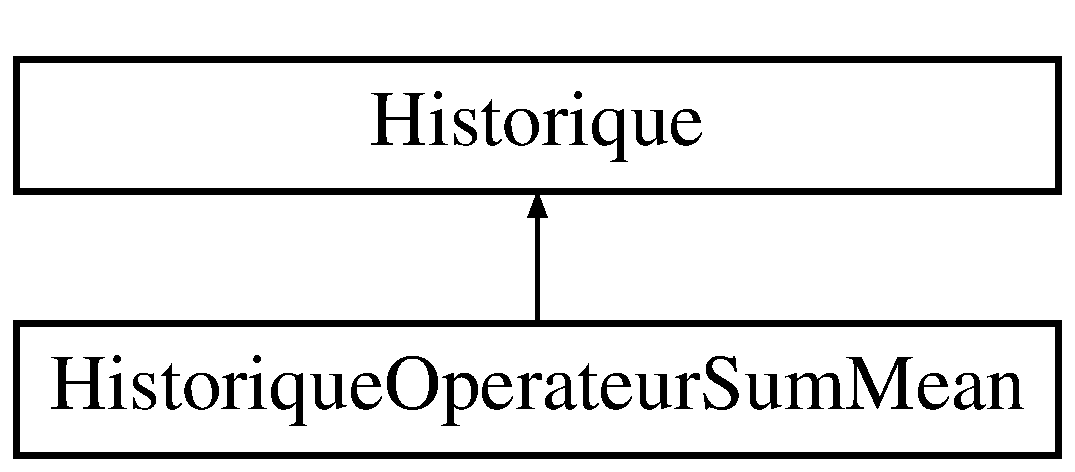
\includegraphics[height=2.000000cm]{class_historique_operateur_sum_mean}
\end{center}
\end{figure}
\subsection*{Public Member Functions}
\begin{DoxyCompactItemize}
\item 
\hyperlink{class_historique_operateur_sum_mean_a5955e29d462ddb6143022ae7cff57c59}{Historique\-Operateur\-Sum\-Mean} (Q\-Stack$<$ \hyperlink{class_constante}{Constante} $\ast$ $>$ $\ast$c1)
\begin{DoxyCompactList}\small\item\em Constructeur avec param�tres. \end{DoxyCompactList}\item 
\hyperlink{class_historique_operateur_sum_mean_a6f85f3aac55f31dcfa734704b89a8893}{$\sim$\-Historique\-Operateur\-Sum\-Mean} ()
\begin{DoxyCompactList}\small\item\em Destructeur de la classe. \end{DoxyCompactList}\item 
\hyperlink{class_constante}{Constante} $\ast$ \hyperlink{class_historique_operateur_sum_mean_a8ab185c12eef9403a26e40c89ce6a830}{set\-Resultat} (\hyperlink{class_constante}{Constante} $\ast$res)
\begin{DoxyCompactList}\small\item\em M�thode permettant de stocker le r�sultat de la commande dans l'attribut \-\_\-resultat de la classe. \end{DoxyCompactList}\item 
void \hyperlink{class_historique_operateur_sum_mean_a5fe3719f36bea1738a0de3ede63f2bf6}{undo} ()
\begin{DoxyCompactList}\small\item\em M�thode virtuelle pure permettant d'effectuer un \char`\"{}undo\char`\"{} sur la commande courante.  \end{DoxyCompactList}\item 
void \hyperlink{class_historique_operateur_sum_mean_a9b6b410f0e49877768d84adfd76da76c}{redo} ()
\begin{DoxyCompactList}\small\item\em M�thode virtuelle pure permettant d'effectuer un \char`\"{}redo\char`\"{} sur la commande courante.  \end{DoxyCompactList}\end{DoxyCompactItemize}


\subsection{Detailed Description}
Classe impl�mentant l'interface \hyperlink{class_historique}{Historique} et permettant de g�rer l'historique des commandes \char`\"{}sum\char`\"{} et \char`\"{}mean\char`\"{}. 

Definition at line 19 of file historique\-Operateur\-Sum\-Mean.\-h.



\subsection{Constructor \& Destructor Documentation}
\hypertarget{class_historique_operateur_sum_mean_a5955e29d462ddb6143022ae7cff57c59}{\index{Historique\-Operateur\-Sum\-Mean@{Historique\-Operateur\-Sum\-Mean}!Historique\-Operateur\-Sum\-Mean@{Historique\-Operateur\-Sum\-Mean}}
\index{Historique\-Operateur\-Sum\-Mean@{Historique\-Operateur\-Sum\-Mean}!HistoriqueOperateurSumMean@{Historique\-Operateur\-Sum\-Mean}}
\subsubsection[{Historique\-Operateur\-Sum\-Mean}]{\setlength{\rightskip}{0pt plus 5cm}{\bf Historique\-Operateur\-Sum\-Mean\-::\-Historique\-Operateur\-Sum\-Mean} (
\begin{DoxyParamCaption}
\item[{Q\-Stack$<$ {\bf Constante} $\ast$ $>$ $\ast$}]{c1}
\end{DoxyParamCaption}
)}}\label{class_historique_operateur_sum_mean_a5955e29d462ddb6143022ae7cff57c59}


Constructeur avec param�tres. 


\begin{DoxyParams}{Parameters}
{\em La} & pile contenant l'ensemble des constantes qui sont somm�es au cours d'un \char`\"{}sum\char`\"{} ou d'un \char`\"{}mean\char`\"{}. \\
\hline
\end{DoxyParams}


Definition at line 4 of file historique\-Operateur\-Sum\-Mean.\-cpp.

\hypertarget{class_historique_operateur_sum_mean_a6f85f3aac55f31dcfa734704b89a8893}{\index{Historique\-Operateur\-Sum\-Mean@{Historique\-Operateur\-Sum\-Mean}!$\sim$\-Historique\-Operateur\-Sum\-Mean@{$\sim$\-Historique\-Operateur\-Sum\-Mean}}
\index{$\sim$\-Historique\-Operateur\-Sum\-Mean@{$\sim$\-Historique\-Operateur\-Sum\-Mean}!HistoriqueOperateurSumMean@{Historique\-Operateur\-Sum\-Mean}}
\subsubsection[{$\sim$\-Historique\-Operateur\-Sum\-Mean}]{\setlength{\rightskip}{0pt plus 5cm}{\bf Historique\-Operateur\-Sum\-Mean\-::$\sim$\-Historique\-Operateur\-Sum\-Mean} (
\begin{DoxyParamCaption}
{}
\end{DoxyParamCaption}
)\hspace{0.3cm}{\ttfamily  \mbox{[}inline\mbox{]}}}}\label{class_historique_operateur_sum_mean_a6f85f3aac55f31dcfa734704b89a8893}


Destructeur de la classe. 



Definition at line 37 of file historique\-Operateur\-Sum\-Mean.\-h.



\subsection{Member Function Documentation}
\hypertarget{class_historique_operateur_sum_mean_a9b6b410f0e49877768d84adfd76da76c}{\index{Historique\-Operateur\-Sum\-Mean@{Historique\-Operateur\-Sum\-Mean}!redo@{redo}}
\index{redo@{redo}!HistoriqueOperateurSumMean@{Historique\-Operateur\-Sum\-Mean}}
\subsubsection[{redo}]{\setlength{\rightskip}{0pt plus 5cm}void {\bf Historique\-Operateur\-Sum\-Mean\-::redo} (
\begin{DoxyParamCaption}
{}
\end{DoxyParamCaption}
)\hspace{0.3cm}{\ttfamily  \mbox{[}virtual\mbox{]}}}}\label{class_historique_operateur_sum_mean_a9b6b410f0e49877768d84adfd76da76c}


M�thode virtuelle pure permettant d'effectuer un \char`\"{}redo\char`\"{} sur la commande courante.  



Implements \hyperlink{class_historique_ad9d996361bf9a68280d8c558da1cd182}{Historique}.



Definition at line 15 of file historique\-Operateur\-Sum\-Mean.\-cpp.

\hypertarget{class_historique_operateur_sum_mean_a8ab185c12eef9403a26e40c89ce6a830}{\index{Historique\-Operateur\-Sum\-Mean@{Historique\-Operateur\-Sum\-Mean}!set\-Resultat@{set\-Resultat}}
\index{set\-Resultat@{set\-Resultat}!HistoriqueOperateurSumMean@{Historique\-Operateur\-Sum\-Mean}}
\subsubsection[{set\-Resultat}]{\setlength{\rightskip}{0pt plus 5cm}{\bf Constante}$\ast$ {\bf Historique\-Operateur\-Sum\-Mean\-::set\-Resultat} (
\begin{DoxyParamCaption}
\item[{{\bf Constante} $\ast$}]{res}
\end{DoxyParamCaption}
)\hspace{0.3cm}{\ttfamily  \mbox{[}inline\mbox{]}}}}\label{class_historique_operateur_sum_mean_a8ab185c12eef9403a26e40c89ce6a830}


M�thode permettant de stocker le r�sultat de la commande dans l'attribut \-\_\-resultat de la classe. 


\begin{DoxyParams}{Parameters}
{\em res} & Le r�sultat de l'op�ration \\
\hline
\end{DoxyParams}
\begin{DoxyReturn}{Returns}
Le r�sultat de l'op�ration 
\end{DoxyReturn}


Definition at line 43 of file historique\-Operateur\-Sum\-Mean.\-h.

\hypertarget{class_historique_operateur_sum_mean_a5fe3719f36bea1738a0de3ede63f2bf6}{\index{Historique\-Operateur\-Sum\-Mean@{Historique\-Operateur\-Sum\-Mean}!undo@{undo}}
\index{undo@{undo}!HistoriqueOperateurSumMean@{Historique\-Operateur\-Sum\-Mean}}
\subsubsection[{undo}]{\setlength{\rightskip}{0pt plus 5cm}void {\bf Historique\-Operateur\-Sum\-Mean\-::undo} (
\begin{DoxyParamCaption}
{}
\end{DoxyParamCaption}
)\hspace{0.3cm}{\ttfamily  \mbox{[}virtual\mbox{]}}}}\label{class_historique_operateur_sum_mean_a5fe3719f36bea1738a0de3ede63f2bf6}


M�thode virtuelle pure permettant d'effectuer un \char`\"{}undo\char`\"{} sur la commande courante.  



Implements \hyperlink{class_historique_ac0247bb67a9535851abe5f76113b4751}{Historique}.



Definition at line 8 of file historique\-Operateur\-Sum\-Mean.\-cpp.



The documentation for this class was generated from the following files\-:\begin{DoxyCompactItemize}
\item 
\hyperlink{historique_operateur_sum_mean_8h}{historique\-Operateur\-Sum\-Mean.\-h}\item 
\hyperlink{historique_operateur_sum_mean_8cpp}{historique\-Operateur\-Sum\-Mean.\-cpp}\end{DoxyCompactItemize}

\hypertarget{class_historique_operateur_swap}{\section{Historique\-Operateur\-Swap Class Reference}
\label{class_historique_operateur_swap}\index{Historique\-Operateur\-Swap@{Historique\-Operateur\-Swap}}
}


Classe impl�mentant l'interface \hyperlink{class_historique}{Historique} et permettant de g�rer l'historique de la commande swap.  




{\ttfamily \#include $<$historique\-Operateur\-Swap.\-h$>$}

Inheritance diagram for Historique\-Operateur\-Swap\-:\begin{figure}[H]
\begin{center}
\leavevmode
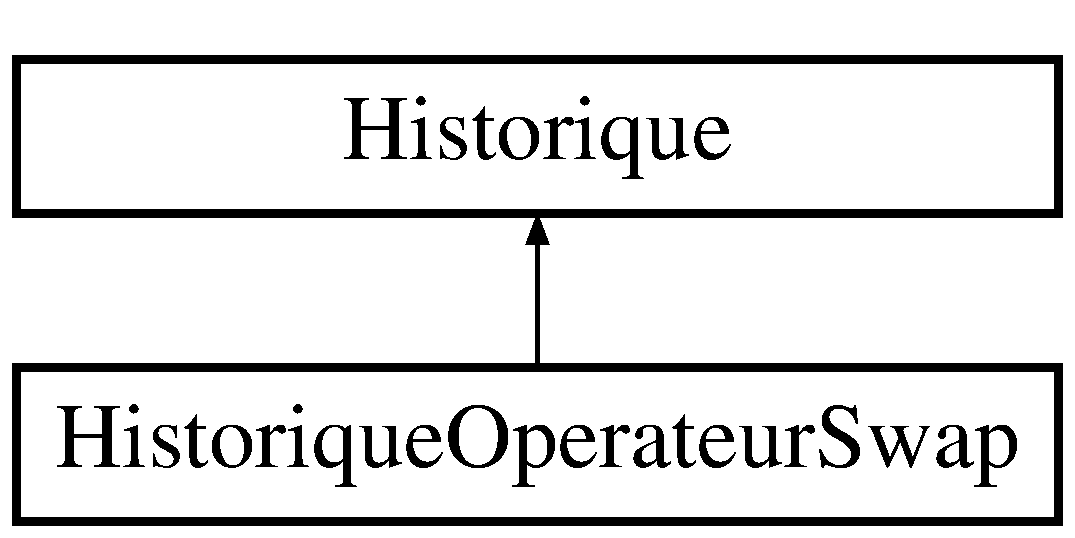
\includegraphics[height=2.000000cm]{class_historique_operateur_swap}
\end{center}
\end{figure}
\subsection*{Public Member Functions}
\begin{DoxyCompactItemize}
\item 
\hyperlink{class_historique_operateur_swap_a8aea2c943abc6254d02e62eb8375928b}{Historique\-Operateur\-Swap} (\hyperlink{class_entier}{Entier} $\ast$c1, \hyperlink{class_entier}{Entier} $\ast$c2)
\begin{DoxyCompactList}\small\item\em Constructeur avec param�tres. \end{DoxyCompactList}\item 
\hyperlink{class_historique_operateur_swap_a00892a4ad9594143a3c955022d281041}{$\sim$\-Historique\-Operateur\-Swap} ()
\begin{DoxyCompactList}\small\item\em Destructeur de la classe. \end{DoxyCompactList}\item 
void \hyperlink{class_historique_operateur_swap_a71cad4d42084faee7a61f21fe93178be}{undo} ()
\begin{DoxyCompactList}\small\item\em M�thode virtuelle pure permettant d'effectuer un \char`\"{}undo\char`\"{} sur la commande courante.  \end{DoxyCompactList}\item 
void \hyperlink{class_historique_operateur_swap_a48aaa552de5396f614974709b5a61e99}{redo} ()
\begin{DoxyCompactList}\small\item\em M�thode virtuelle pure permettant d'effectuer un \char`\"{}redo\char`\"{} sur la commande courante.  \end{DoxyCompactList}\end{DoxyCompactItemize}


\subsection{Detailed Description}
Classe impl�mentant l'interface \hyperlink{class_historique}{Historique} et permettant de g�rer l'historique de la commande swap. 

Definition at line 18 of file historique\-Operateur\-Swap.\-h.



\subsection{Constructor \& Destructor Documentation}
\hypertarget{class_historique_operateur_swap_a8aea2c943abc6254d02e62eb8375928b}{\index{Historique\-Operateur\-Swap@{Historique\-Operateur\-Swap}!Historique\-Operateur\-Swap@{Historique\-Operateur\-Swap}}
\index{Historique\-Operateur\-Swap@{Historique\-Operateur\-Swap}!HistoriqueOperateurSwap@{Historique\-Operateur\-Swap}}
\subsubsection[{Historique\-Operateur\-Swap}]{\setlength{\rightskip}{0pt plus 5cm}{\bf Historique\-Operateur\-Swap\-::\-Historique\-Operateur\-Swap} (
\begin{DoxyParamCaption}
\item[{{\bf Entier} $\ast$}]{c1, }
\item[{{\bf Entier} $\ast$}]{c2}
\end{DoxyParamCaption}
)\hspace{0.3cm}{\ttfamily  \mbox{[}inline\mbox{]}}}}\label{class_historique_operateur_swap_a8aea2c943abc6254d02e62eb8375928b}


Constructeur avec param�tres. 


\begin{DoxyParams}{Parameters}
{\em c1} & Le premier indice du swap \\
\hline
{\em c2} & Le second indice du swap \\
\hline
\end{DoxyParams}


Definition at line 33 of file historique\-Operateur\-Swap.\-h.

\hypertarget{class_historique_operateur_swap_a00892a4ad9594143a3c955022d281041}{\index{Historique\-Operateur\-Swap@{Historique\-Operateur\-Swap}!$\sim$\-Historique\-Operateur\-Swap@{$\sim$\-Historique\-Operateur\-Swap}}
\index{$\sim$\-Historique\-Operateur\-Swap@{$\sim$\-Historique\-Operateur\-Swap}!HistoriqueOperateurSwap@{Historique\-Operateur\-Swap}}
\subsubsection[{$\sim$\-Historique\-Operateur\-Swap}]{\setlength{\rightskip}{0pt plus 5cm}{\bf Historique\-Operateur\-Swap\-::$\sim$\-Historique\-Operateur\-Swap} (
\begin{DoxyParamCaption}
{}
\end{DoxyParamCaption}
)\hspace{0.3cm}{\ttfamily  \mbox{[}inline\mbox{]}}}}\label{class_historique_operateur_swap_a00892a4ad9594143a3c955022d281041}


Destructeur de la classe. 



Definition at line 37 of file historique\-Operateur\-Swap.\-h.



\subsection{Member Function Documentation}
\hypertarget{class_historique_operateur_swap_a48aaa552de5396f614974709b5a61e99}{\index{Historique\-Operateur\-Swap@{Historique\-Operateur\-Swap}!redo@{redo}}
\index{redo@{redo}!HistoriqueOperateurSwap@{Historique\-Operateur\-Swap}}
\subsubsection[{redo}]{\setlength{\rightskip}{0pt plus 5cm}void {\bf Historique\-Operateur\-Swap\-::redo} (
\begin{DoxyParamCaption}
{}
\end{DoxyParamCaption}
)\hspace{0.3cm}{\ttfamily  \mbox{[}virtual\mbox{]}}}}\label{class_historique_operateur_swap_a48aaa552de5396f614974709b5a61e99}


M�thode virtuelle pure permettant d'effectuer un \char`\"{}redo\char`\"{} sur la commande courante.  



Implements \hyperlink{class_historique_ad9d996361bf9a68280d8c558da1cd182}{Historique}.



Definition at line 8 of file historique\-Operateur\-Swap.\-cpp.

\hypertarget{class_historique_operateur_swap_a71cad4d42084faee7a61f21fe93178be}{\index{Historique\-Operateur\-Swap@{Historique\-Operateur\-Swap}!undo@{undo}}
\index{undo@{undo}!HistoriqueOperateurSwap@{Historique\-Operateur\-Swap}}
\subsubsection[{undo}]{\setlength{\rightskip}{0pt plus 5cm}void {\bf Historique\-Operateur\-Swap\-::undo} (
\begin{DoxyParamCaption}
{}
\end{DoxyParamCaption}
)\hspace{0.3cm}{\ttfamily  \mbox{[}virtual\mbox{]}}}}\label{class_historique_operateur_swap_a71cad4d42084faee7a61f21fe93178be}


M�thode virtuelle pure permettant d'effectuer un \char`\"{}undo\char`\"{} sur la commande courante.  



Implements \hyperlink{class_historique_ac0247bb67a9535851abe5f76113b4751}{Historique}.



Definition at line 4 of file historique\-Operateur\-Swap.\-cpp.



The documentation for this class was generated from the following files\-:\begin{DoxyCompactItemize}
\item 
\hyperlink{historique_operateur_swap_8h}{historique\-Operateur\-Swap.\-h}\item 
\hyperlink{historique_operateur_swap_8cpp}{historique\-Operateur\-Swap.\-cpp}\end{DoxyCompactItemize}

\hypertarget{class_historique_operateur_unaire}{\section{Historique\-Operateur\-Unaire Class Reference}
\label{class_historique_operateur_unaire}\index{Historique\-Operateur\-Unaire@{Historique\-Operateur\-Unaire}}
}


Classe impl�mentant l'interface \hyperlink{class_historique}{Historique} et permettant de g�rer l'historique des commandes unaires.  




{\ttfamily \#include $<$historique\-Operateur\-Unaire.\-h$>$}

Inheritance diagram for Historique\-Operateur\-Unaire\-:\begin{figure}[H]
\begin{center}
\leavevmode
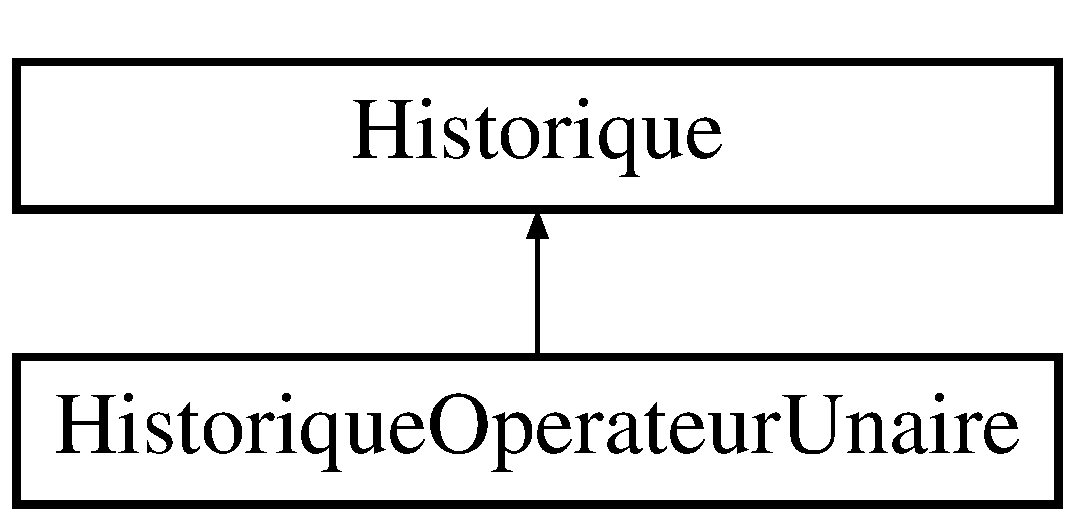
\includegraphics[height=2.000000cm]{class_historique_operateur_unaire}
\end{center}
\end{figure}
\subsection*{Public Member Functions}
\begin{DoxyCompactItemize}
\item 
\hyperlink{class_historique_operateur_unaire_a9cc77c41baf02f48499556f38a32cdfc}{Historique\-Operateur\-Unaire} (\hyperlink{class_constante}{Constante} $\ast$c1)
\begin{DoxyCompactList}\small\item\em Le constructeur avec param�tres. \end{DoxyCompactList}\item 
\hyperlink{class_historique_operateur_unaire_aa3cde907f3765b17ea0769efad4adb63}{$\sim$\-Historique\-Operateur\-Unaire} ()
\begin{DoxyCompactList}\small\item\em Destructeur de la classe. \end{DoxyCompactList}\item 
\hyperlink{class_constante}{Constante} $\ast$ \hyperlink{class_historique_operateur_unaire_a5b538df2478095236db252ea80106163}{set\-Resultat} (\hyperlink{class_constante}{Constante} $\ast$res)
\begin{DoxyCompactList}\small\item\em M�thode permettant de stocker le r�sultat de la commande dans l'attribut \-\_\-resultat de la classe. \end{DoxyCompactList}\item 
void \hyperlink{class_historique_operateur_unaire_aebd86086fd2ce41cd529035a8140c262}{undo} ()
\begin{DoxyCompactList}\small\item\em M�thode virtuelle pure permettant d'effectuer un \char`\"{}undo\char`\"{} sur la commande courante.  \end{DoxyCompactList}\item 
void \hyperlink{class_historique_operateur_unaire_a57f9d18a4a6ece2a9bb4797003c6f6bc}{redo} ()
\begin{DoxyCompactList}\small\item\em M�thode virtuelle pure permettant d'effectuer un \char`\"{}redo\char`\"{} sur la commande courante.  \end{DoxyCompactList}\end{DoxyCompactItemize}


\subsection{Detailed Description}
Classe impl�mentant l'interface \hyperlink{class_historique}{Historique} et permettant de g�rer l'historique des commandes unaires. 

Definition at line 18 of file historique\-Operateur\-Unaire.\-h.



\subsection{Constructor \& Destructor Documentation}
\hypertarget{class_historique_operateur_unaire_a9cc77c41baf02f48499556f38a32cdfc}{\index{Historique\-Operateur\-Unaire@{Historique\-Operateur\-Unaire}!Historique\-Operateur\-Unaire@{Historique\-Operateur\-Unaire}}
\index{Historique\-Operateur\-Unaire@{Historique\-Operateur\-Unaire}!HistoriqueOperateurUnaire@{Historique\-Operateur\-Unaire}}
\subsubsection[{Historique\-Operateur\-Unaire}]{\setlength{\rightskip}{0pt plus 5cm}{\bf Historique\-Operateur\-Unaire\-::\-Historique\-Operateur\-Unaire} (
\begin{DoxyParamCaption}
\item[{{\bf Constante} $\ast$}]{c1}
\end{DoxyParamCaption}
)\hspace{0.3cm}{\ttfamily  \mbox{[}inline\mbox{]}}}}\label{class_historique_operateur_unaire_a9cc77c41baf02f48499556f38a32cdfc}


Le constructeur avec param�tres. 


\begin{DoxyParams}{Parameters}
{\em c1} & L'op�rande de l'op�ration \\
\hline
\end{DoxyParams}


Definition at line 32 of file historique\-Operateur\-Unaire.\-h.

\hypertarget{class_historique_operateur_unaire_aa3cde907f3765b17ea0769efad4adb63}{\index{Historique\-Operateur\-Unaire@{Historique\-Operateur\-Unaire}!$\sim$\-Historique\-Operateur\-Unaire@{$\sim$\-Historique\-Operateur\-Unaire}}
\index{$\sim$\-Historique\-Operateur\-Unaire@{$\sim$\-Historique\-Operateur\-Unaire}!HistoriqueOperateurUnaire@{Historique\-Operateur\-Unaire}}
\subsubsection[{$\sim$\-Historique\-Operateur\-Unaire}]{\setlength{\rightskip}{0pt plus 5cm}{\bf Historique\-Operateur\-Unaire\-::$\sim$\-Historique\-Operateur\-Unaire} (
\begin{DoxyParamCaption}
{}
\end{DoxyParamCaption}
)\hspace{0.3cm}{\ttfamily  \mbox{[}inline\mbox{]}}}}\label{class_historique_operateur_unaire_aa3cde907f3765b17ea0769efad4adb63}


Destructeur de la classe. 



Definition at line 36 of file historique\-Operateur\-Unaire.\-h.



\subsection{Member Function Documentation}
\hypertarget{class_historique_operateur_unaire_a57f9d18a4a6ece2a9bb4797003c6f6bc}{\index{Historique\-Operateur\-Unaire@{Historique\-Operateur\-Unaire}!redo@{redo}}
\index{redo@{redo}!HistoriqueOperateurUnaire@{Historique\-Operateur\-Unaire}}
\subsubsection[{redo}]{\setlength{\rightskip}{0pt plus 5cm}void {\bf Historique\-Operateur\-Unaire\-::redo} (
\begin{DoxyParamCaption}
{}
\end{DoxyParamCaption}
)\hspace{0.3cm}{\ttfamily  \mbox{[}virtual\mbox{]}}}}\label{class_historique_operateur_unaire_a57f9d18a4a6ece2a9bb4797003c6f6bc}


M�thode virtuelle pure permettant d'effectuer un \char`\"{}redo\char`\"{} sur la commande courante.  



Implements \hyperlink{class_historique_ad9d996361bf9a68280d8c558da1cd182}{Historique}.



Definition at line 9 of file historique\-Operateur\-Unaire.\-cpp.

\hypertarget{class_historique_operateur_unaire_a5b538df2478095236db252ea80106163}{\index{Historique\-Operateur\-Unaire@{Historique\-Operateur\-Unaire}!set\-Resultat@{set\-Resultat}}
\index{set\-Resultat@{set\-Resultat}!HistoriqueOperateurUnaire@{Historique\-Operateur\-Unaire}}
\subsubsection[{set\-Resultat}]{\setlength{\rightskip}{0pt plus 5cm}{\bf Constante}$\ast$ {\bf Historique\-Operateur\-Unaire\-::set\-Resultat} (
\begin{DoxyParamCaption}
\item[{{\bf Constante} $\ast$}]{res}
\end{DoxyParamCaption}
)\hspace{0.3cm}{\ttfamily  \mbox{[}inline\mbox{]}}}}\label{class_historique_operateur_unaire_a5b538df2478095236db252ea80106163}


M�thode permettant de stocker le r�sultat de la commande dans l'attribut \-\_\-resultat de la classe. 


\begin{DoxyParams}{Parameters}
{\em res} & Le r�sultat de l'op�ration \\
\hline
\end{DoxyParams}
\begin{DoxyReturn}{Returns}
Le r�sultat de l'op�ration 
\end{DoxyReturn}


Definition at line 42 of file historique\-Operateur\-Unaire.\-h.

\hypertarget{class_historique_operateur_unaire_aebd86086fd2ce41cd529035a8140c262}{\index{Historique\-Operateur\-Unaire@{Historique\-Operateur\-Unaire}!undo@{undo}}
\index{undo@{undo}!HistoriqueOperateurUnaire@{Historique\-Operateur\-Unaire}}
\subsubsection[{undo}]{\setlength{\rightskip}{0pt plus 5cm}void {\bf Historique\-Operateur\-Unaire\-::undo} (
\begin{DoxyParamCaption}
{}
\end{DoxyParamCaption}
)\hspace{0.3cm}{\ttfamily  \mbox{[}virtual\mbox{]}}}}\label{class_historique_operateur_unaire_aebd86086fd2ce41cd529035a8140c262}


M�thode virtuelle pure permettant d'effectuer un \char`\"{}undo\char`\"{} sur la commande courante.  



Implements \hyperlink{class_historique_ac0247bb67a9535851abe5f76113b4751}{Historique}.



Definition at line 4 of file historique\-Operateur\-Unaire.\-cpp.



The documentation for this class was generated from the following files\-:\begin{DoxyCompactItemize}
\item 
\hyperlink{historique_operateur_unaire_8h}{historique\-Operateur\-Unaire.\-h}\item 
\hyperlink{historique_operateur_unaire_8cpp}{historique\-Operateur\-Unaire.\-cpp}\end{DoxyCompactItemize}

\hypertarget{class_log_message}{\section{Log\-Message Class Reference}
\label{class_log_message}\index{Log\-Message@{Log\-Message}}
}


Classe permettant de g�rer un message de Log (son contenu et son degre d'importance).  




{\ttfamily \#include $<$log\-Message.\-h$>$}

\subsection*{Public Member Functions}
\begin{DoxyCompactItemize}
\item 
\hyperlink{class_log_message_a4839b5003c888431a491b118c9962596}{Log\-Message} ()
\begin{DoxyCompactList}\small\item\em Constructeur par d�faut. \end{DoxyCompactList}\item 
\hyperlink{class_log_message_abd764a1d00d85b796495cfc997903c1c}{Log\-Message} (const Q\-String \&mes, int degre)
\begin{DoxyCompactList}\small\item\em Constructeur avec param�tres. \end{DoxyCompactList}\item 
Q\-String \hyperlink{class_log_message_acc855cee5e2033d264b3ed830d9a0939}{get\-Message} () const 
\begin{DoxyCompactList}\small\item\em Getter du contenu du message. \end{DoxyCompactList}\item 
int \hyperlink{class_log_message_aeabac2d8e6eae50747a6369a85eb207d}{get\-Degre} () const 
\begin{DoxyCompactList}\small\item\em Getter de l'importance du message. \end{DoxyCompactList}\item 
Q\-String \hyperlink{class_log_message_ac7c710b7c6c46180673d953507308e89}{get\-Date} () const 
\begin{DoxyCompactList}\small\item\em Getter de la date du message. \end{DoxyCompactList}\end{DoxyCompactItemize}


\subsection{Detailed Description}
Classe permettant de g�rer un message de Log (son contenu et son degre d'importance). 

Definition at line 18 of file log\-Message.\-h.



\subsection{Constructor \& Destructor Documentation}
\hypertarget{class_log_message_a4839b5003c888431a491b118c9962596}{\index{Log\-Message@{Log\-Message}!Log\-Message@{Log\-Message}}
\index{Log\-Message@{Log\-Message}!LogMessage@{Log\-Message}}
\subsubsection[{Log\-Message}]{\setlength{\rightskip}{0pt plus 5cm}{\bf Log\-Message\-::\-Log\-Message} (
\begin{DoxyParamCaption}
{}
\end{DoxyParamCaption}
)}}\label{class_log_message_a4839b5003c888431a491b118c9962596}


Constructeur par d�faut. 

\hypertarget{class_log_message_abd764a1d00d85b796495cfc997903c1c}{\index{Log\-Message@{Log\-Message}!Log\-Message@{Log\-Message}}
\index{Log\-Message@{Log\-Message}!LogMessage@{Log\-Message}}
\subsubsection[{Log\-Message}]{\setlength{\rightskip}{0pt plus 5cm}{\bf Log\-Message\-::\-Log\-Message} (
\begin{DoxyParamCaption}
\item[{const Q\-String \&}]{mes, }
\item[{int}]{degre}
\end{DoxyParamCaption}
)\hspace{0.3cm}{\ttfamily  \mbox{[}inline\mbox{]}}}}\label{class_log_message_abd764a1d00d85b796495cfc997903c1c}


Constructeur avec param�tres. 


\begin{DoxyParams}{Parameters}
{\em mes} & string \\
\hline
{\em degre} & int \\
\hline
\end{DoxyParams}


Definition at line 42 of file log\-Message.\-h.



\subsection{Member Function Documentation}
\hypertarget{class_log_message_ac7c710b7c6c46180673d953507308e89}{\index{Log\-Message@{Log\-Message}!get\-Date@{get\-Date}}
\index{get\-Date@{get\-Date}!LogMessage@{Log\-Message}}
\subsubsection[{get\-Date}]{\setlength{\rightskip}{0pt plus 5cm}Q\-String {\bf Log\-Message\-::get\-Date} (
\begin{DoxyParamCaption}
{}
\end{DoxyParamCaption}
) const\hspace{0.3cm}{\ttfamily  \mbox{[}inline\mbox{]}}}}\label{class_log_message_ac7c710b7c6c46180673d953507308e89}


Getter de la date du message. 

\begin{DoxyReturn}{Returns}
La date du message 
\end{DoxyReturn}


Definition at line 62 of file log\-Message.\-h.

\hypertarget{class_log_message_aeabac2d8e6eae50747a6369a85eb207d}{\index{Log\-Message@{Log\-Message}!get\-Degre@{get\-Degre}}
\index{get\-Degre@{get\-Degre}!LogMessage@{Log\-Message}}
\subsubsection[{get\-Degre}]{\setlength{\rightskip}{0pt plus 5cm}int {\bf Log\-Message\-::get\-Degre} (
\begin{DoxyParamCaption}
{}
\end{DoxyParamCaption}
) const\hspace{0.3cm}{\ttfamily  \mbox{[}inline\mbox{]}}}}\label{class_log_message_aeabac2d8e6eae50747a6369a85eb207d}


Getter de l'importance du message. 

\begin{DoxyReturn}{Returns}
L'importance du message 
\end{DoxyReturn}


Definition at line 57 of file log\-Message.\-h.

\hypertarget{class_log_message_acc855cee5e2033d264b3ed830d9a0939}{\index{Log\-Message@{Log\-Message}!get\-Message@{get\-Message}}
\index{get\-Message@{get\-Message}!LogMessage@{Log\-Message}}
\subsubsection[{get\-Message}]{\setlength{\rightskip}{0pt plus 5cm}Q\-String {\bf Log\-Message\-::get\-Message} (
\begin{DoxyParamCaption}
{}
\end{DoxyParamCaption}
) const\hspace{0.3cm}{\ttfamily  \mbox{[}inline\mbox{]}}}}\label{class_log_message_acc855cee5e2033d264b3ed830d9a0939}


Getter du contenu du message. 

\begin{DoxyReturn}{Returns}
Le contenu du message 
\end{DoxyReturn}


Definition at line 52 of file log\-Message.\-h.



The documentation for this class was generated from the following file\-:\begin{DoxyCompactItemize}
\item 
\hyperlink{log_message_8h}{log\-Message.\-h}\end{DoxyCompactItemize}

\hypertarget{class_log_system}{\section{Log\-System Class Reference}
\label{class_log_system}\index{Log\-System@{Log\-System}}
}


Classe (utilisant le Design Pattern Singleton) permettant de g�rer l'�criture des messages de log dans le fichier correspondant.  




{\ttfamily \#include $<$log\-System.\-h$>$}

\subsection*{Public Member Functions}
\begin{DoxyCompactItemize}
\item 
void \hyperlink{class_log_system_a38444fac316292c4288405ae11491cd4}{add\-Message} (const \hyperlink{class_log_message}{Log\-Message} \&log)
\begin{DoxyCompactList}\small\item\em M�thode permettant d'�crire un message\-Log dans le fichier de Log. \end{DoxyCompactList}\item 
void \hyperlink{class_log_system_ae207ba8afc4d2ea32a7e3e8c8dcf2048}{reset} ()
\begin{DoxyCompactList}\small\item\em M�thode permettant de r�initialiser le fichier de log. \end{DoxyCompactList}\item 
Q\-String \hyperlink{class_log_system_aa80c476e8d2bd057887665f5438735a0}{initialisation\-Fichier} ()
\begin{DoxyCompactList}\small\item\em M�thode permettant d'�tablir l'ent�te du fichier. \end{DoxyCompactList}\end{DoxyCompactItemize}
\subsection*{Static Public Member Functions}
\begin{DoxyCompactItemize}
\item 
static \hyperlink{class_log_system}{Log\-System} $\ast$ \hyperlink{class_log_system_a787ad45b69b64fb8f883555bd4f0ba93}{get\-Instance} ()
\begin{DoxyCompactList}\small\item\em M�thode permettant d'acc�der � l'instance de la classe \hyperlink{class_log_system}{Log\-System}. \end{DoxyCompactList}\item 
static void \hyperlink{class_log_system_ace6193771588639979fb177c4fa47b4e}{free\-Instance} ()
\begin{DoxyCompactList}\small\item\em M�thode permettant de lib�rer l'instance de la classe \hyperlink{class_log_system}{Log\-System}. \end{DoxyCompactList}\end{DoxyCompactItemize}


\subsection{Detailed Description}
Classe (utilisant le Design Pattern Singleton) permettant de g�rer l'�criture des messages de log dans le fichier correspondant. 

Definition at line 20 of file log\-System.\-h.



\subsection{Member Function Documentation}
\hypertarget{class_log_system_a38444fac316292c4288405ae11491cd4}{\index{Log\-System@{Log\-System}!add\-Message@{add\-Message}}
\index{add\-Message@{add\-Message}!LogSystem@{Log\-System}}
\subsubsection[{add\-Message}]{\setlength{\rightskip}{0pt plus 5cm}void {\bf Log\-System\-::add\-Message} (
\begin{DoxyParamCaption}
\item[{const {\bf Log\-Message} \&}]{log}
\end{DoxyParamCaption}
)}}\label{class_log_system_a38444fac316292c4288405ae11491cd4}


M�thode permettant d'�crire un message\-Log dans le fichier de Log. 


\begin{DoxyParams}{Parameters}
{\em log} & Le message � ajouter dans le fichier de log mais aussi sur l'interface graphique. \\
\hline
\end{DoxyParams}
\begin{DoxyReturn}{Returns}
void 
\end{DoxyReturn}


Definition at line 40 of file log\-System.\-cpp.

\hypertarget{class_log_system_ace6193771588639979fb177c4fa47b4e}{\index{Log\-System@{Log\-System}!free\-Instance@{free\-Instance}}
\index{free\-Instance@{free\-Instance}!LogSystem@{Log\-System}}
\subsubsection[{free\-Instance}]{\setlength{\rightskip}{0pt plus 5cm}void {\bf Log\-System\-::free\-Instance} (
\begin{DoxyParamCaption}
{}
\end{DoxyParamCaption}
)\hspace{0.3cm}{\ttfamily  \mbox{[}static\mbox{]}}}}\label{class_log_system_ace6193771588639979fb177c4fa47b4e}


M�thode permettant de lib�rer l'instance de la classe \hyperlink{class_log_system}{Log\-System}. 

\begin{DoxyReturn}{Returns}
void 
\end{DoxyReturn}


Definition at line 31 of file log\-System.\-cpp.

\hypertarget{class_log_system_a787ad45b69b64fb8f883555bd4f0ba93}{\index{Log\-System@{Log\-System}!get\-Instance@{get\-Instance}}
\index{get\-Instance@{get\-Instance}!LogSystem@{Log\-System}}
\subsubsection[{get\-Instance}]{\setlength{\rightskip}{0pt plus 5cm}{\bf Log\-System} $\ast$ {\bf Log\-System\-::get\-Instance} (
\begin{DoxyParamCaption}
{}
\end{DoxyParamCaption}
)\hspace{0.3cm}{\ttfamily  \mbox{[}static\mbox{]}}}}\label{class_log_system_a787ad45b69b64fb8f883555bd4f0ba93}


M�thode permettant d'acc�der � l'instance de la classe \hyperlink{class_log_system}{Log\-System}. 

\begin{DoxyReturn}{Returns}
instance de \hyperlink{class_log_system}{Log\-System} 
\end{DoxyReturn}


Definition at line 26 of file log\-System.\-cpp.

\hypertarget{class_log_system_aa80c476e8d2bd057887665f5438735a0}{\index{Log\-System@{Log\-System}!initialisation\-Fichier@{initialisation\-Fichier}}
\index{initialisation\-Fichier@{initialisation\-Fichier}!LogSystem@{Log\-System}}
\subsubsection[{initialisation\-Fichier}]{\setlength{\rightskip}{0pt plus 5cm}Q\-String {\bf Log\-System\-::initialisation\-Fichier} (
\begin{DoxyParamCaption}
{}
\end{DoxyParamCaption}
)}}\label{class_log_system_aa80c476e8d2bd057887665f5438735a0}


M�thode permettant d'�tablir l'ent�te du fichier. 

\begin{DoxyReturn}{Returns}
La chaine contenant l'entete du fichier 
\end{DoxyReturn}


Definition at line 72 of file log\-System.\-cpp.

\hypertarget{class_log_system_ae207ba8afc4d2ea32a7e3e8c8dcf2048}{\index{Log\-System@{Log\-System}!reset@{reset}}
\index{reset@{reset}!LogSystem@{Log\-System}}
\subsubsection[{reset}]{\setlength{\rightskip}{0pt plus 5cm}void {\bf Log\-System\-::reset} (
\begin{DoxyParamCaption}
{}
\end{DoxyParamCaption}
)}}\label{class_log_system_ae207ba8afc4d2ea32a7e3e8c8dcf2048}


M�thode permettant de r�initialiser le fichier de log. 



Definition at line 64 of file log\-System.\-cpp.



The documentation for this class was generated from the following files\-:\begin{DoxyCompactItemize}
\item 
\hyperlink{log_system_8h}{log\-System.\-h}\item 
\hyperlink{log_system_8cpp}{log\-System.\-cpp}\end{DoxyCompactItemize}

\hypertarget{class_main_window}{\section{Main\-Window Class Reference}
\label{class_main_window}\index{Main\-Window@{Main\-Window}}
}


Classe (utilisant le Design Pattern Singleton) permettant de g�rer l'interface de la calculatrice, ainsi que les interactions entre celle-\/ci et les classes associ�es.  




{\ttfamily \#include $<$mainwindow.\-h$>$}

\subsection*{Public Member Functions}
\begin{DoxyCompactItemize}
\item 
void \hyperlink{class_main_window_a58135ab8b13869a0ac40aa110c0914eb}{charger\-Contexte} ()
\begin{DoxyCompactList}\small\item\em M�thode permettant de charger le contexte \-: cad charger les bons param�tres en fonction des settings. \end{DoxyCompactList}\item 
\hyperlink{class_pile}{Pile} $\ast$ \hyperlink{class_main_window_aafa30e84f5163a63323a7fb3a960199e}{get\-Pile} () const 
\begin{DoxyCompactList}\small\item\em Getter permettant de retourner la pile utilis�. \end{DoxyCompactList}\item 
void \hyperlink{class_main_window_ad75c14f8c8d8c5f3591f6286f6df71a8}{set\-Stack\-Display\-Spin\-Box} (int i)
\begin{DoxyCompactList}\small\item\em M�thode permettant de fixer le nombre d'�l�ments de la pile � afficher. \end{DoxyCompactList}\item 
void \hyperlink{class_main_window_a431d6a7fd08fac994cd0740f4f58eac8}{set\-Input\-Line\-Edit} (const Q\-String \&str)
\begin{DoxyCompactList}\small\item\em M�thode permettant de modifier le contenu du champ de saisie par la string en param�tre, et appelle la m�thode permettant de traiter cette chaine. \end{DoxyCompactList}\item 
void \hyperlink{class_main_window_a8cf3c5ca6532158f321ff234ad5fca58}{set\-Stack\-Display\-Text\-Edit} (const Q\-String \&str)
\begin{DoxyCompactList}\small\item\em M�thode permettant d'ajouter \char`\"{}str\char`\"{} au contenu d�j� pr�sent dans le champ de saisie. \end{DoxyCompactList}\end{DoxyCompactItemize}
\subsection*{Static Public Member Functions}
\begin{DoxyCompactItemize}
\item 
static \hyperlink{class_main_window}{Main\-Window} $\ast$ \hyperlink{class_main_window_adbe77fe06e8ee3324c38577a79b4eed6}{get\-Instance} ()
\begin{DoxyCompactList}\small\item\em M�thode permettant de retourner l'instance de la classe. \end{DoxyCompactList}\item 
static void \hyperlink{class_main_window_afdf126bf06f3b9828eb6653cc3d37603}{free\-Instance} ()
\begin{DoxyCompactList}\small\item\em M�thode permettant de lib�rer l'instance de classe. \end{DoxyCompactList}\end{DoxyCompactItemize}


\subsection{Detailed Description}
Classe (utilisant le Design Pattern Singleton) permettant de g�rer l'interface de la calculatrice, ainsi que les interactions entre celle-\/ci et les classes associ�es. 

Definition at line 30 of file mainwindow.\-h.



\subsection{Member Function Documentation}
\hypertarget{class_main_window_a58135ab8b13869a0ac40aa110c0914eb}{\index{Main\-Window@{Main\-Window}!charger\-Contexte@{charger\-Contexte}}
\index{charger\-Contexte@{charger\-Contexte}!MainWindow@{Main\-Window}}
\subsubsection[{charger\-Contexte}]{\setlength{\rightskip}{0pt plus 5cm}void {\bf Main\-Window\-::charger\-Contexte} (
\begin{DoxyParamCaption}
{}
\end{DoxyParamCaption}
)}}\label{class_main_window_a58135ab8b13869a0ac40aa110c0914eb}


M�thode permettant de charger le contexte \-: cad charger les bons param�tres en fonction des settings. 



Definition at line 27 of file mainwindow.\-cpp.

\hypertarget{class_main_window_afdf126bf06f3b9828eb6653cc3d37603}{\index{Main\-Window@{Main\-Window}!free\-Instance@{free\-Instance}}
\index{free\-Instance@{free\-Instance}!MainWindow@{Main\-Window}}
\subsubsection[{free\-Instance}]{\setlength{\rightskip}{0pt plus 5cm}void {\bf Main\-Window\-::free\-Instance} (
\begin{DoxyParamCaption}
{}
\end{DoxyParamCaption}
)\hspace{0.3cm}{\ttfamily  \mbox{[}static\mbox{]}}}}\label{class_main_window_afdf126bf06f3b9828eb6653cc3d37603}


M�thode permettant de lib�rer l'instance de classe. 



Definition at line 54 of file mainwindow.\-cpp.

\hypertarget{class_main_window_adbe77fe06e8ee3324c38577a79b4eed6}{\index{Main\-Window@{Main\-Window}!get\-Instance@{get\-Instance}}
\index{get\-Instance@{get\-Instance}!MainWindow@{Main\-Window}}
\subsubsection[{get\-Instance}]{\setlength{\rightskip}{0pt plus 5cm}{\bf Main\-Window} $\ast$ {\bf Main\-Window\-::get\-Instance} (
\begin{DoxyParamCaption}
{}
\end{DoxyParamCaption}
)\hspace{0.3cm}{\ttfamily  \mbox{[}static\mbox{]}}}}\label{class_main_window_adbe77fe06e8ee3324c38577a79b4eed6}


M�thode permettant de retourner l'instance de la classe. 

\begin{DoxyReturn}{Returns}
L'instance de la classe 
\end{DoxyReturn}


Definition at line 48 of file mainwindow.\-cpp.

\hypertarget{class_main_window_aafa30e84f5163a63323a7fb3a960199e}{\index{Main\-Window@{Main\-Window}!get\-Pile@{get\-Pile}}
\index{get\-Pile@{get\-Pile}!MainWindow@{Main\-Window}}
\subsubsection[{get\-Pile}]{\setlength{\rightskip}{0pt plus 5cm}{\bf Pile}$\ast$ {\bf Main\-Window\-::get\-Pile} (
\begin{DoxyParamCaption}
{}
\end{DoxyParamCaption}
) const\hspace{0.3cm}{\ttfamily  \mbox{[}inline\mbox{]}}}}\label{class_main_window_aafa30e84f5163a63323a7fb3a960199e}


Getter permettant de retourner la pile utilis�. 

\begin{DoxyReturn}{Returns}
La pile de la calculatrice 
\end{DoxyReturn}


Definition at line 72 of file mainwindow.\-h.

\hypertarget{class_main_window_a431d6a7fd08fac994cd0740f4f58eac8}{\index{Main\-Window@{Main\-Window}!set\-Input\-Line\-Edit@{set\-Input\-Line\-Edit}}
\index{set\-Input\-Line\-Edit@{set\-Input\-Line\-Edit}!MainWindow@{Main\-Window}}
\subsubsection[{set\-Input\-Line\-Edit}]{\setlength{\rightskip}{0pt plus 5cm}void {\bf Main\-Window\-::set\-Input\-Line\-Edit} (
\begin{DoxyParamCaption}
\item[{const Q\-String \&}]{str}
\end{DoxyParamCaption}
)}}\label{class_main_window_a431d6a7fd08fac994cd0740f4f58eac8}


M�thode permettant de modifier le contenu du champ de saisie par la string en param�tre, et appelle la m�thode permettant de traiter cette chaine. 


\begin{DoxyParams}{Parameters}
{\em str} & La chaine de caract�res � ins�rer \\
\hline
\end{DoxyParams}


Definition at line 508 of file mainwindow.\-cpp.

\hypertarget{class_main_window_ad75c14f8c8d8c5f3591f6286f6df71a8}{\index{Main\-Window@{Main\-Window}!set\-Stack\-Display\-Spin\-Box@{set\-Stack\-Display\-Spin\-Box}}
\index{set\-Stack\-Display\-Spin\-Box@{set\-Stack\-Display\-Spin\-Box}!MainWindow@{Main\-Window}}
\subsubsection[{set\-Stack\-Display\-Spin\-Box}]{\setlength{\rightskip}{0pt plus 5cm}void {\bf Main\-Window\-::set\-Stack\-Display\-Spin\-Box} (
\begin{DoxyParamCaption}
\item[{int}]{i}
\end{DoxyParamCaption}
)}}\label{class_main_window_ad75c14f8c8d8c5f3591f6286f6df71a8}


M�thode permettant de fixer le nombre d'�l�ments de la pile � afficher. 


\begin{DoxyParams}{Parameters}
{\em i} & Le nombre d'�l�ments � afficher \\
\hline
\end{DoxyParams}


Definition at line 504 of file mainwindow.\-cpp.

\hypertarget{class_main_window_a8cf3c5ca6532158f321ff234ad5fca58}{\index{Main\-Window@{Main\-Window}!set\-Stack\-Display\-Text\-Edit@{set\-Stack\-Display\-Text\-Edit}}
\index{set\-Stack\-Display\-Text\-Edit@{set\-Stack\-Display\-Text\-Edit}!MainWindow@{Main\-Window}}
\subsubsection[{set\-Stack\-Display\-Text\-Edit}]{\setlength{\rightskip}{0pt plus 5cm}void {\bf Main\-Window\-::set\-Stack\-Display\-Text\-Edit} (
\begin{DoxyParamCaption}
\item[{const Q\-String \&}]{str}
\end{DoxyParamCaption}
)}}\label{class_main_window_a8cf3c5ca6532158f321ff234ad5fca58}


M�thode permettant d'ajouter \char`\"{}str\char`\"{} au contenu d�j� pr�sent dans le champ de saisie. 


\begin{DoxyParams}{Parameters}
{\em str} & La chaine de caract�res � ajouter \\
\hline
\end{DoxyParams}


Definition at line 500 of file mainwindow.\-cpp.



The documentation for this class was generated from the following files\-:\begin{DoxyCompactItemize}
\item 
\hyperlink{mainwindow_8h}{mainwindow.\-h}\item 
\hyperlink{mainwindow_8cpp}{mainwindow.\-cpp}\end{DoxyCompactItemize}

\hypertarget{class_nombre}{\section{Nombre Class Reference}
\label{class_nombre}\index{Nombre@{Nombre}}
}


Classe qui �tend l'interface \hyperlink{class_constante}{Constante} pour regrouper tout les valeurs de type num�rique sous cette classe et �galement de proposer les diff�rentes op�rations sp�cifiques aux nombres (op�rations arithm�tiques, etc).  




{\ttfamily \#include $<$nombre.\-h$>$}

Inheritance diagram for Nombre\-:\begin{figure}[H]
\begin{center}
\leavevmode
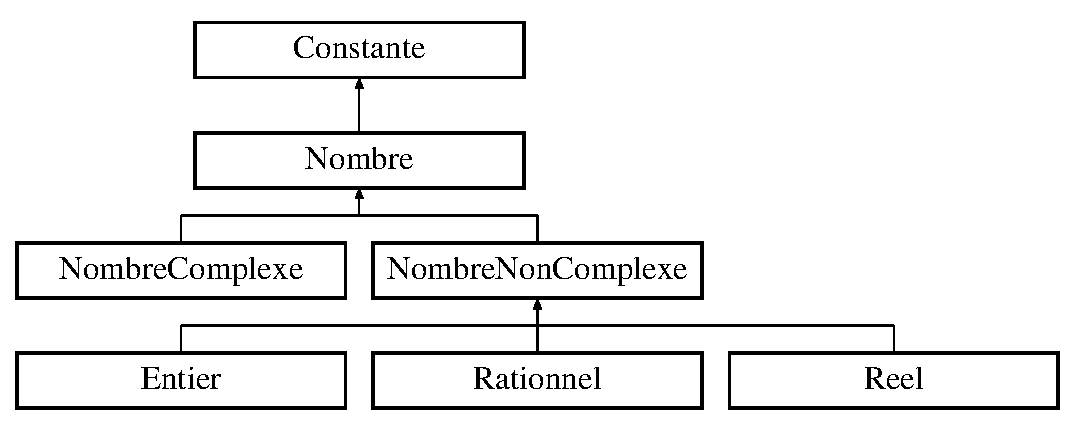
\includegraphics[height=4.000000cm]{class_nombre}
\end{center}
\end{figure}
\subsection*{Public Member Functions}
\begin{DoxyCompactItemize}
\item 
virtual \hyperlink{class_nombre_a4c6b76d82eb43d78f09ef09ac96e68c3}{$\sim$\-Nombre} ()
\begin{DoxyCompactList}\small\item\em Destructeur de classe. \end{DoxyCompactList}\item 
virtual void \hyperlink{class_nombre_a718d616bbf2e5e8f133df958e8bb3d7f}{sign} ()=0
\begin{DoxyCompactList}\small\item\em Methode permettant de transformer le nombre en son oppos�. \end{DoxyCompactList}\item 
virtual void \hyperlink{class_nombre_a5be0e66e9bbec508d236ba8dbe1eb6bc}{sqr} ()=0
\begin{DoxyCompactList}\small\item\em M�thode permettant de transformer le nombre en son carr�. \end{DoxyCompactList}\item 
virtual void \hyperlink{class_nombre_aed65cb1449858c078e91610afb3a6447}{cube} ()=0
\begin{DoxyCompactList}\small\item\em M�thode permettant de transformer le nombre en son cube. \end{DoxyCompactList}\item 
virtual \hyperlink{class_nombre_complexe}{Nombre\-Complexe} $\ast$ \hyperlink{class_nombre_a11092e1fcde81c05b4c518398baf3691}{to\-Nombre\-Complexe} ()=0
\begin{DoxyCompactList}\small\item\em M�thode permettant de convertir un \hyperlink{class_nombre}{Nombre} en son �quivalent en \hyperlink{class_nombre_complexe}{Nombre\-Complexe}. \end{DoxyCompactList}\item 
\hyperlink{class_expression}{Expression} $\ast$ \hyperlink{class_nombre_aa1f5526edb56eae2e40c17632670bed6}{operator+} (\hyperlink{class_expression}{Expression} $\ast$e)
\begin{DoxyCompactList}\small\item\em M�thode permettant de retourner une expression contenant l'expression appelante, la constante pass�e en param�tre et ainsi que l'op�rateur associ� ('+').  \end{DoxyCompactList}\item 
\hyperlink{class_expression}{Expression} $\ast$ \hyperlink{class_nombre_af71f33adeab91851ffcc15cad121d8c2}{operator-\/} (\hyperlink{class_expression}{Expression} $\ast$e)
\begin{DoxyCompactList}\small\item\em M�thode permettant de retourner une expression contenant l'expression appelante, la constante pass�e en param�tre et ainsi que l'op�rateur associ� ('-\/').  \end{DoxyCompactList}\item 
\hyperlink{class_expression}{Expression} $\ast$ \hyperlink{class_nombre_ab1ba55765b198cda277000d6b80403a5}{operator/} (\hyperlink{class_expression}{Expression} $\ast$e)
\begin{DoxyCompactList}\small\item\em M�thode permettant de retourner une expression contenant l'expression appelante, la constante pass�e en param�tre et ainsi que l'op�rateur associ� ('/').  \end{DoxyCompactList}\item 
\hyperlink{class_expression}{Expression} $\ast$ \hyperlink{class_nombre_ab99de52caa404260195eea417158edb5}{operator$\ast$} (\hyperlink{class_expression}{Expression} $\ast$e)
\begin{DoxyCompactList}\small\item\em M�thode permettant de retourner une expression contenant l'expression appelante, la constante pass�e en param�tre et ainsi que l'op�rateur associ� ('$\ast$').  \end{DoxyCompactList}\item 
\hyperlink{class_constante}{Constante} $\ast$ \hyperlink{class_nombre_a229c1d79d365612f92108fbfeb90edc3}{Acos} ()  throw (\-Log\-Message)
\begin{DoxyCompactList}\small\item\em M�thode permettant de calculer le cos sur un \hyperlink{class_nombre}{Nombre}. \end{DoxyCompactList}\item 
\hyperlink{class_constante}{Constante} $\ast$ \hyperlink{class_nombre_a4d9ff32a9e30b511360c72bc6c1e88fb}{Asin} ()  throw (\-Log\-Message)
\begin{DoxyCompactList}\small\item\em M�thode permettant de calculer le sin sur un \hyperlink{class_nombre}{Nombre}. \end{DoxyCompactList}\item 
\hyperlink{class_constante}{Constante} $\ast$ \hyperlink{class_nombre_a41e4de9cae8eb7dbb92618d9d60e2407}{Atan} ()  throw (\-Log\-Message)
\begin{DoxyCompactList}\small\item\em M�thode permettant d'appliquer la tan sur un \hyperlink{class_nombre}{Nombre}. \end{DoxyCompactList}\item 
\hyperlink{class_constante}{Constante} $\ast$ \hyperlink{class_nombre_aa404e08423be432dbbc33dcf065ef121}{Asinh} ()  throw (\-Log\-Message)
\begin{DoxyCompactList}\small\item\em M�thode permettant de calculer le sinush sur un \hyperlink{class_nombre}{Nombre}. \end{DoxyCompactList}\item 
\hyperlink{class_constante}{Constante} $\ast$ \hyperlink{class_nombre_afe078f44711c53b620b2f230fc14000e}{Acosh} ()  throw (\-Log\-Message)
\begin{DoxyCompactList}\small\item\em M�thode permettant de calculer le cosh sur un \hyperlink{class_nombre}{Nombre}. \end{DoxyCompactList}\item 
\hyperlink{class_constante}{Constante} $\ast$ \hyperlink{class_nombre_a39146b14a1b90e07f743cafa5654f4ac}{Atanh} ()  throw (\-Log\-Message)
\begin{DoxyCompactList}\small\item\em M�thode permettant de calculer le tanh sur un \hyperlink{class_nombre}{Nombre}. \end{DoxyCompactList}\item 
\hyperlink{class_constante}{Constante} $\ast$ \hyperlink{class_nombre_a43fba9af9a6945b25c4911844e55f6eb}{Aln} ()  throw (\-Log\-Message)
\begin{DoxyCompactList}\small\item\em M�thode permettant de calculer le logarithme n�p�rien sur un \hyperlink{class_nombre}{Nombre}. \end{DoxyCompactList}\item 
\hyperlink{class_constante}{Constante} $\ast$ \hyperlink{class_nombre_ae08b484b5c2749c5887e912f3a3b4b76}{Alog} ()  throw (\-Log\-Message)
\begin{DoxyCompactList}\small\item\em M�thode permettant de calculer le logarithme sur un \hyperlink{class_nombre}{Nombre}. \end{DoxyCompactList}\item 
\hyperlink{class_constante}{Constante} $\ast$ \hyperlink{class_nombre_a1b25dae06f854558c169ba44c162b815}{Ainv} ()  throw (\-Log\-Message)
\begin{DoxyCompactList}\small\item\em M�thode permettant de retourner l'inverse d'un \hyperlink{class_nombre}{Nombre}. \end{DoxyCompactList}\item 
\hyperlink{class_constante}{Constante} $\ast$ \hyperlink{class_nombre_abd9749ce16130bd71b8990c6660b70c3}{Asqrt} ()  throw (\-Log\-Message)
\begin{DoxyCompactList}\small\item\em M�thode permettant de calculer la racine d'un \hyperlink{class_nombre}{Nombre}. \end{DoxyCompactList}\end{DoxyCompactItemize}


\subsection{Detailed Description}
Classe qui �tend l'interface \hyperlink{class_constante}{Constante} pour regrouper tout les valeurs de type num�rique sous cette classe et �galement de proposer les diff�rentes op�rations sp�cifiques aux nombres (op�rations arithm�tiques, etc). 

Definition at line 22 of file nombre.\-h.



\subsection{Constructor \& Destructor Documentation}
\hypertarget{class_nombre_a4c6b76d82eb43d78f09ef09ac96e68c3}{\index{Nombre@{Nombre}!$\sim$\-Nombre@{$\sim$\-Nombre}}
\index{$\sim$\-Nombre@{$\sim$\-Nombre}!Nombre@{Nombre}}
\subsubsection[{$\sim$\-Nombre}]{\setlength{\rightskip}{0pt plus 5cm}virtual {\bf Nombre\-::$\sim$\-Nombre} (
\begin{DoxyParamCaption}
{}
\end{DoxyParamCaption}
)\hspace{0.3cm}{\ttfamily  \mbox{[}inline, virtual\mbox{]}}}}\label{class_nombre_a4c6b76d82eb43d78f09ef09ac96e68c3}


Destructeur de classe. 



Definition at line 28 of file nombre.\-h.



\subsection{Member Function Documentation}
\hypertarget{class_nombre_a229c1d79d365612f92108fbfeb90edc3}{\index{Nombre@{Nombre}!Acos@{Acos}}
\index{Acos@{Acos}!Nombre@{Nombre}}
\subsubsection[{Acos}]{\setlength{\rightskip}{0pt plus 5cm}{\bf Constante} $\ast$ {\bf Nombre\-::\-Acos} (
\begin{DoxyParamCaption}
{}
\end{DoxyParamCaption}
)  throw ({\bf Log\-Message})}}\label{class_nombre_a229c1d79d365612f92108fbfeb90edc3}


M�thode permettant de calculer le cos sur un \hyperlink{class_nombre}{Nombre}. 

\begin{DoxyReturn}{Returns}
La constante contenant le cos du \hyperlink{class_nombre}{Nombre} en tenant compte des param�tres utilisateurs (R\-A\-D\-I\-A\-N ou D\-E\-G\-R\-E\-S). 
\end{DoxyReturn}


Definition at line 48 of file nombre.\-cpp.

\hypertarget{class_nombre_afe078f44711c53b620b2f230fc14000e}{\index{Nombre@{Nombre}!Acosh@{Acosh}}
\index{Acosh@{Acosh}!Nombre@{Nombre}}
\subsubsection[{Acosh}]{\setlength{\rightskip}{0pt plus 5cm}{\bf Constante} $\ast$ {\bf Nombre\-::\-Acosh} (
\begin{DoxyParamCaption}
{}
\end{DoxyParamCaption}
)  throw ({\bf Log\-Message})}}\label{class_nombre_afe078f44711c53b620b2f230fc14000e}


M�thode permettant de calculer le cosh sur un \hyperlink{class_nombre}{Nombre}. 

\begin{DoxyReturn}{Returns}
La constante contenant le cosh du \hyperlink{class_nombre}{Nombre} en tenant compte des param�tres utilisateurs (R\-A\-D\-I\-A\-N ou D\-E\-G\-R\-E\-S). 
\end{DoxyReturn}


Definition at line 116 of file nombre.\-cpp.

\hypertarget{class_nombre_a1b25dae06f854558c169ba44c162b815}{\index{Nombre@{Nombre}!Ainv@{Ainv}}
\index{Ainv@{Ainv}!Nombre@{Nombre}}
\subsubsection[{Ainv}]{\setlength{\rightskip}{0pt plus 5cm}{\bf Constante} $\ast$ {\bf Nombre\-::\-Ainv} (
\begin{DoxyParamCaption}
{}
\end{DoxyParamCaption}
)  throw ({\bf Log\-Message})}}\label{class_nombre_a1b25dae06f854558c169ba44c162b815}


M�thode permettant de retourner l'inverse d'un \hyperlink{class_nombre}{Nombre}. 

\begin{DoxyReturn}{Returns}
La constante contenant l'inverse du \hyperlink{class_nombre}{Nombre}. 
\end{DoxyReturn}


Definition at line 197 of file nombre.\-cpp.

\hypertarget{class_nombre_a43fba9af9a6945b25c4911844e55f6eb}{\index{Nombre@{Nombre}!Aln@{Aln}}
\index{Aln@{Aln}!Nombre@{Nombre}}
\subsubsection[{Aln}]{\setlength{\rightskip}{0pt plus 5cm}{\bf Constante} $\ast$ {\bf Nombre\-::\-Aln} (
\begin{DoxyParamCaption}
{}
\end{DoxyParamCaption}
)  throw ({\bf Log\-Message})}}\label{class_nombre_a43fba9af9a6945b25c4911844e55f6eb}


M�thode permettant de calculer le logarithme n�p�rien sur un \hyperlink{class_nombre}{Nombre}. 

\begin{DoxyReturn}{Returns}
La constante contenant le logarithme n�p�rien du \hyperlink{class_nombre}{Nombre}. 
\end{DoxyReturn}


Definition at line 156 of file nombre.\-cpp.

\hypertarget{class_nombre_ae08b484b5c2749c5887e912f3a3b4b76}{\index{Nombre@{Nombre}!Alog@{Alog}}
\index{Alog@{Alog}!Nombre@{Nombre}}
\subsubsection[{Alog}]{\setlength{\rightskip}{0pt plus 5cm}{\bf Constante} $\ast$ {\bf Nombre\-::\-Alog} (
\begin{DoxyParamCaption}
{}
\end{DoxyParamCaption}
)  throw ({\bf Log\-Message})}}\label{class_nombre_ae08b484b5c2749c5887e912f3a3b4b76}


M�thode permettant de calculer le logarithme sur un \hyperlink{class_nombre}{Nombre}. 

\begin{DoxyReturn}{Returns}
La constante contenant le logarithme du \hyperlink{class_nombre}{Nombre}. 
\end{DoxyReturn}


Definition at line 176 of file nombre.\-cpp.

\hypertarget{class_nombre_a4d9ff32a9e30b511360c72bc6c1e88fb}{\index{Nombre@{Nombre}!Asin@{Asin}}
\index{Asin@{Asin}!Nombre@{Nombre}}
\subsubsection[{Asin}]{\setlength{\rightskip}{0pt plus 5cm}{\bf Constante} $\ast$ {\bf Nombre\-::\-Asin} (
\begin{DoxyParamCaption}
{}
\end{DoxyParamCaption}
)  throw ({\bf Log\-Message})}}\label{class_nombre_a4d9ff32a9e30b511360c72bc6c1e88fb}


M�thode permettant de calculer le sin sur un \hyperlink{class_nombre}{Nombre}. 

\begin{DoxyReturn}{Returns}
La constante contenant le sin du \hyperlink{class_nombre}{Nombre} en tenant compte des param�tres utilisateurs (R\-A\-D\-I\-A\-N ou D\-E\-G\-R\-E\-S). 
\end{DoxyReturn}


Definition at line 24 of file nombre.\-cpp.

\hypertarget{class_nombre_aa404e08423be432dbbc33dcf065ef121}{\index{Nombre@{Nombre}!Asinh@{Asinh}}
\index{Asinh@{Asinh}!Nombre@{Nombre}}
\subsubsection[{Asinh}]{\setlength{\rightskip}{0pt plus 5cm}{\bf Constante} $\ast$ {\bf Nombre\-::\-Asinh} (
\begin{DoxyParamCaption}
{}
\end{DoxyParamCaption}
)  throw ({\bf Log\-Message})}}\label{class_nombre_aa404e08423be432dbbc33dcf065ef121}


M�thode permettant de calculer le sinush sur un \hyperlink{class_nombre}{Nombre}. 

\begin{DoxyReturn}{Returns}
La constante contenant le sinush du \hyperlink{class_nombre}{Nombre} en tenant compte des param�tres utilisateurs (R\-A\-D\-I\-A\-N ou D\-E\-G\-R\-E\-S). 
\end{DoxyReturn}


Definition at line 96 of file nombre.\-cpp.

\hypertarget{class_nombre_abd9749ce16130bd71b8990c6660b70c3}{\index{Nombre@{Nombre}!Asqrt@{Asqrt}}
\index{Asqrt@{Asqrt}!Nombre@{Nombre}}
\subsubsection[{Asqrt}]{\setlength{\rightskip}{0pt plus 5cm}{\bf Constante} $\ast$ {\bf Nombre\-::\-Asqrt} (
\begin{DoxyParamCaption}
{}
\end{DoxyParamCaption}
)  throw ({\bf Log\-Message})}}\label{class_nombre_abd9749ce16130bd71b8990c6660b70c3}


M�thode permettant de calculer la racine d'un \hyperlink{class_nombre}{Nombre}. 

\begin{DoxyReturn}{Returns}
La constante contenant la racine du \hyperlink{class_nombre}{Nombre}. 
\end{DoxyReturn}


Definition at line 222 of file nombre.\-cpp.

\hypertarget{class_nombre_a41e4de9cae8eb7dbb92618d9d60e2407}{\index{Nombre@{Nombre}!Atan@{Atan}}
\index{Atan@{Atan}!Nombre@{Nombre}}
\subsubsection[{Atan}]{\setlength{\rightskip}{0pt plus 5cm}{\bf Constante} $\ast$ {\bf Nombre\-::\-Atan} (
\begin{DoxyParamCaption}
{}
\end{DoxyParamCaption}
)  throw ({\bf Log\-Message})}}\label{class_nombre_a41e4de9cae8eb7dbb92618d9d60e2407}


M�thode permettant d'appliquer la tan sur un \hyperlink{class_nombre}{Nombre}. 

\begin{DoxyReturn}{Returns}
La constante contenant la tan du \hyperlink{class_nombre}{Nombre} en tenant compte des param�tres utilisateurs (R\-A\-D\-I\-A\-N ou D\-E\-G\-R\-E\-S). 
\end{DoxyReturn}


Definition at line 72 of file nombre.\-cpp.

\hypertarget{class_nombre_a39146b14a1b90e07f743cafa5654f4ac}{\index{Nombre@{Nombre}!Atanh@{Atanh}}
\index{Atanh@{Atanh}!Nombre@{Nombre}}
\subsubsection[{Atanh}]{\setlength{\rightskip}{0pt plus 5cm}{\bf Constante} $\ast$ {\bf Nombre\-::\-Atanh} (
\begin{DoxyParamCaption}
{}
\end{DoxyParamCaption}
)  throw ({\bf Log\-Message})}}\label{class_nombre_a39146b14a1b90e07f743cafa5654f4ac}


M�thode permettant de calculer le tanh sur un \hyperlink{class_nombre}{Nombre}. 

\begin{DoxyReturn}{Returns}
La constante contenant le tanh du \hyperlink{class_nombre}{Nombre} en tenant compte des param�tres utilisateurs (R\-A\-D\-I\-A\-N ou D\-E\-G\-R\-E\-S). 
\end{DoxyReturn}


Definition at line 136 of file nombre.\-cpp.

\hypertarget{class_nombre_aed65cb1449858c078e91610afb3a6447}{\index{Nombre@{Nombre}!cube@{cube}}
\index{cube@{cube}!Nombre@{Nombre}}
\subsubsection[{cube}]{\setlength{\rightskip}{0pt plus 5cm}virtual void {\bf Nombre\-::cube} (
\begin{DoxyParamCaption}
{}
\end{DoxyParamCaption}
)\hspace{0.3cm}{\ttfamily  \mbox{[}pure virtual\mbox{]}}}}\label{class_nombre_aed65cb1449858c078e91610afb3a6447}


M�thode permettant de transformer le nombre en son cube. 



Implemented in \hyperlink{class_rationnel_a72bf5e2bac1e10990d44783b8d2d7ab1}{Rationnel}, \hyperlink{class_entier_a8fbf1379f26622554393e48df17867fd}{Entier}, \hyperlink{class_nombre_complexe_ae6e43b7eec06f92933e8f54571e383e6}{Nombre\-Complexe}, and \hyperlink{class_reel_ac46be5621787809b3fea257b54fee83f}{Reel}.

\hypertarget{class_nombre_ab99de52caa404260195eea417158edb5}{\index{Nombre@{Nombre}!operator$\ast$@{operator$\ast$}}
\index{operator$\ast$@{operator$\ast$}!Nombre@{Nombre}}
\subsubsection[{operator$\ast$}]{\setlength{\rightskip}{0pt plus 5cm}{\bf Expression} $\ast$ Nombre\-::operator$\ast$ (
\begin{DoxyParamCaption}
\item[{{\bf Expression} $\ast$}]{e}
\end{DoxyParamCaption}
)}}\label{class_nombre_ab99de52caa404260195eea417158edb5}


M�thode permettant de retourner une expression contenant l'expression appelante, la constante pass�e en param�tre et ainsi que l'op�rateur associ� ('$\ast$').  


\begin{DoxyParams}{Parameters}
{\em c} & La constante � ins�rer dans l'expression \\
\hline
\end{DoxyParams}
\begin{DoxyReturn}{Returns}
L'expression ressortissante de l'op�ration 
\end{DoxyReturn}
 

Definition at line 20 of file nombre.\-cpp.

\hypertarget{class_nombre_aa1f5526edb56eae2e40c17632670bed6}{\index{Nombre@{Nombre}!operator+@{operator+}}
\index{operator+@{operator+}!Nombre@{Nombre}}
\subsubsection[{operator+}]{\setlength{\rightskip}{0pt plus 5cm}{\bf Expression} $\ast$ Nombre\-::operator+ (
\begin{DoxyParamCaption}
\item[{{\bf Expression} $\ast$}]{e}
\end{DoxyParamCaption}
)}}\label{class_nombre_aa1f5526edb56eae2e40c17632670bed6}


M�thode permettant de retourner une expression contenant l'expression appelante, la constante pass�e en param�tre et ainsi que l'op�rateur associ� ('+').  


\begin{DoxyParams}{Parameters}
{\em c} & La constante � ins�rer dans l'expression \\
\hline
\end{DoxyParams}
\begin{DoxyReturn}{Returns}
L'expression ressortissante de l'op�ration 
\end{DoxyReturn}
 

Definition at line 8 of file nombre.\-cpp.

\hypertarget{class_nombre_af71f33adeab91851ffcc15cad121d8c2}{\index{Nombre@{Nombre}!operator-\/@{operator-\/}}
\index{operator-\/@{operator-\/}!Nombre@{Nombre}}
\subsubsection[{operator-\/}]{\setlength{\rightskip}{0pt plus 5cm}{\bf Expression} $\ast$ Nombre\-::operator-\/ (
\begin{DoxyParamCaption}
\item[{{\bf Expression} $\ast$}]{e}
\end{DoxyParamCaption}
)}}\label{class_nombre_af71f33adeab91851ffcc15cad121d8c2}


M�thode permettant de retourner une expression contenant l'expression appelante, la constante pass�e en param�tre et ainsi que l'op�rateur associ� ('-\/').  


\begin{DoxyParams}{Parameters}
{\em c} & La constante � ins�rer dans l'expression \\
\hline
\end{DoxyParams}
\begin{DoxyReturn}{Returns}
L'expression ressortissante de l'op�ration 
\end{DoxyReturn}
 

Definition at line 12 of file nombre.\-cpp.

\hypertarget{class_nombre_ab1ba55765b198cda277000d6b80403a5}{\index{Nombre@{Nombre}!operator/@{operator/}}
\index{operator/@{operator/}!Nombre@{Nombre}}
\subsubsection[{operator/}]{\setlength{\rightskip}{0pt plus 5cm}{\bf Expression} $\ast$ Nombre\-::operator/ (
\begin{DoxyParamCaption}
\item[{{\bf Expression} $\ast$}]{e}
\end{DoxyParamCaption}
)}}\label{class_nombre_ab1ba55765b198cda277000d6b80403a5}


M�thode permettant de retourner une expression contenant l'expression appelante, la constante pass�e en param�tre et ainsi que l'op�rateur associ� ('/').  


\begin{DoxyParams}{Parameters}
{\em c} & La constante � ins�rer dans l'expression \\
\hline
\end{DoxyParams}
\begin{DoxyReturn}{Returns}
L'expression ressortissante de l'op�ration 
\end{DoxyReturn}
 

Definition at line 16 of file nombre.\-cpp.

\hypertarget{class_nombre_a718d616bbf2e5e8f133df958e8bb3d7f}{\index{Nombre@{Nombre}!sign@{sign}}
\index{sign@{sign}!Nombre@{Nombre}}
\subsubsection[{sign}]{\setlength{\rightskip}{0pt plus 5cm}virtual void {\bf Nombre\-::sign} (
\begin{DoxyParamCaption}
{}
\end{DoxyParamCaption}
)\hspace{0.3cm}{\ttfamily  \mbox{[}pure virtual\mbox{]}}}}\label{class_nombre_a718d616bbf2e5e8f133df958e8bb3d7f}


Methode permettant de transformer le nombre en son oppos�. 



Implemented in \hyperlink{class_rationnel_a723b922369bb264764b319fde37068d7}{Rationnel}, \hyperlink{class_entier_a91748c3918f8eed1c188f5175328cf1a}{Entier}, \hyperlink{class_nombre_complexe_ae81bf4639b5fbbb27f20204720a38489}{Nombre\-Complexe}, and \hyperlink{class_reel_ab86c394e2e4a6729ecafba23e65915ad}{Reel}.

\hypertarget{class_nombre_a5be0e66e9bbec508d236ba8dbe1eb6bc}{\index{Nombre@{Nombre}!sqr@{sqr}}
\index{sqr@{sqr}!Nombre@{Nombre}}
\subsubsection[{sqr}]{\setlength{\rightskip}{0pt plus 5cm}virtual void {\bf Nombre\-::sqr} (
\begin{DoxyParamCaption}
{}
\end{DoxyParamCaption}
)\hspace{0.3cm}{\ttfamily  \mbox{[}pure virtual\mbox{]}}}}\label{class_nombre_a5be0e66e9bbec508d236ba8dbe1eb6bc}


M�thode permettant de transformer le nombre en son carr�. 



Implemented in \hyperlink{class_rationnel_acb4195e9590b74f9895398f69acc7692}{Rationnel}, \hyperlink{class_entier_a66dff979b86690f26360fd3a93b25537}{Entier}, \hyperlink{class_nombre_complexe_aca52852015c47d4c8246fbf3c9cebd62}{Nombre\-Complexe}, and \hyperlink{class_reel_a612dd1edfce0d6fa687ab4cbfc700d07}{Reel}.

\hypertarget{class_nombre_a11092e1fcde81c05b4c518398baf3691}{\index{Nombre@{Nombre}!to\-Nombre\-Complexe@{to\-Nombre\-Complexe}}
\index{to\-Nombre\-Complexe@{to\-Nombre\-Complexe}!Nombre@{Nombre}}
\subsubsection[{to\-Nombre\-Complexe}]{\setlength{\rightskip}{0pt plus 5cm}virtual {\bf Nombre\-Complexe}$\ast$ {\bf Nombre\-::to\-Nombre\-Complexe} (
\begin{DoxyParamCaption}
{}
\end{DoxyParamCaption}
)\hspace{0.3cm}{\ttfamily  \mbox{[}pure virtual\mbox{]}}}}\label{class_nombre_a11092e1fcde81c05b4c518398baf3691}


M�thode permettant de convertir un \hyperlink{class_nombre}{Nombre} en son �quivalent en \hyperlink{class_nombre_complexe}{Nombre\-Complexe}. 

\begin{DoxyReturn}{Returns}
Le pointeur vers le nombre\-Complexe nouvellement cr�e 
\end{DoxyReturn}


Implemented in \hyperlink{class_nombre_complexe_a10a9ca96f5d1a1d6ebff4099befca807}{Nombre\-Complexe}, \hyperlink{class_entier_abadca482fe27a3302f874e9e7c109579}{Entier}, \hyperlink{class_rationnel_a06771fbd968456d02a56480ba3a12bc6}{Rationnel}, and \hyperlink{class_reel_a3ba5e47699a1ccff32075a588afda91e}{Reel}.



The documentation for this class was generated from the following files\-:\begin{DoxyCompactItemize}
\item 
\hyperlink{nombre_8h}{nombre.\-h}\item 
\hyperlink{nombre_8cpp}{nombre.\-cpp}\end{DoxyCompactItemize}

\hypertarget{class_nombre_complexe}{\section{Nombre\-Complexe Class Reference}
\label{class_nombre_complexe}\index{Nombre\-Complexe@{Nombre\-Complexe}}
}


Classe impl�mentant l'interface \hyperlink{class_nombre}{Nombre} et permettant de g�rer des constantes de type complexe.  




{\ttfamily \#include $<$nombre\-Complexe.\-h$>$}

Inheritance diagram for Nombre\-Complexe\-:\begin{figure}[H]
\begin{center}
\leavevmode
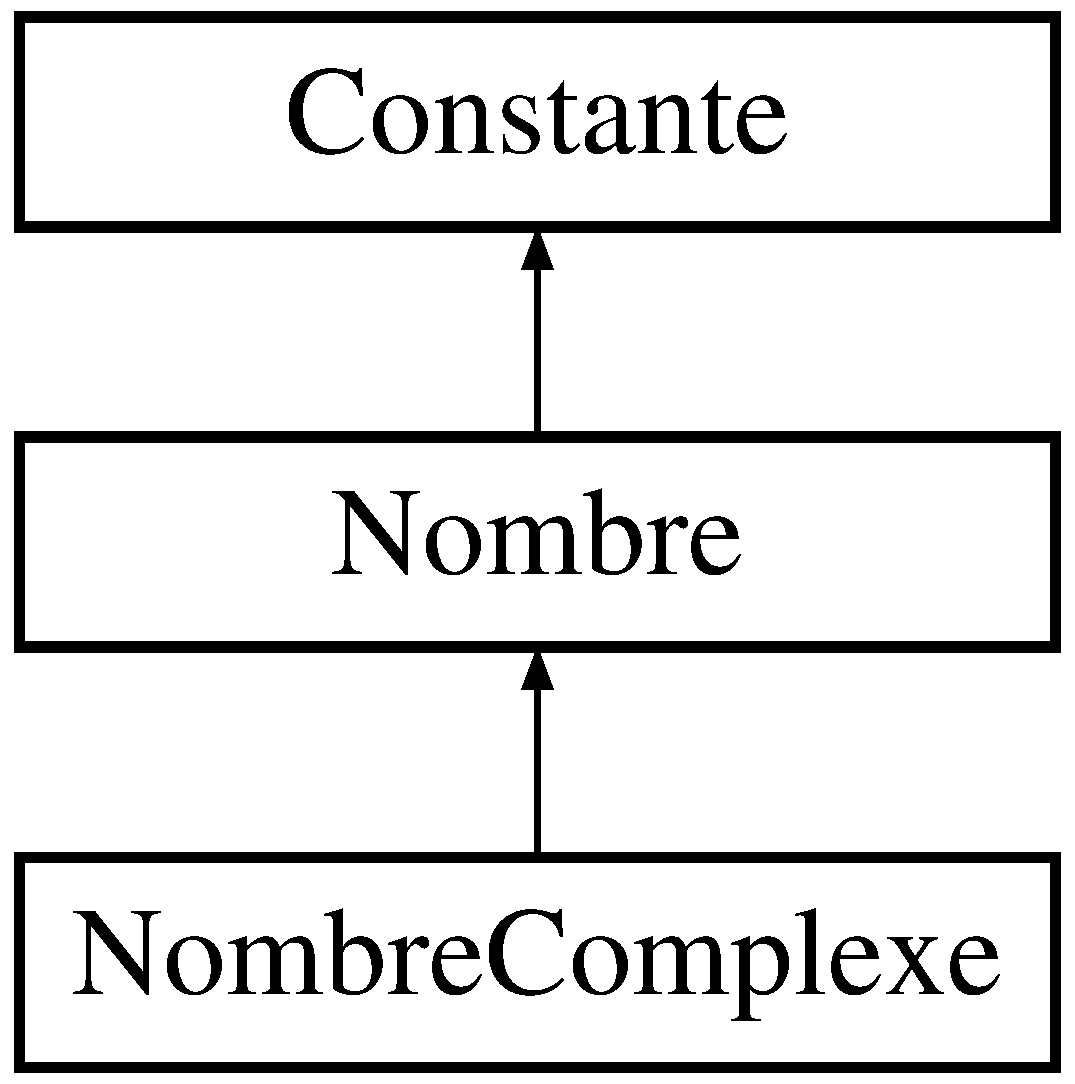
\includegraphics[height=3.000000cm]{class_nombre_complexe}
\end{center}
\end{figure}
\subsection*{Public Member Functions}
\begin{DoxyCompactItemize}
\item 
\hyperlink{class_nombre_complexe_a3d8003eb3008536fab415f5155405ed9}{Nombre\-Complexe} ()
\begin{DoxyCompactList}\small\item\em Cr�e un nombre complexe. \end{DoxyCompactList}\item 
\hyperlink{class_nombre_complexe_a263fa61a4b065844b5c535485068ab6a}{Nombre\-Complexe} (\hyperlink{class_nombre_non_complexe}{Nombre\-Non\-Complexe} $\ast$reel, \hyperlink{class_nombre_non_complexe}{Nombre\-Non\-Complexe} $\ast$img)
\begin{DoxyCompactList}\small\item\em Cr�e un nombre complexe. \end{DoxyCompactList}\item 
\hyperlink{class_nombre_complexe}{Nombre\-Complexe} $\ast$ \hyperlink{class_nombre_complexe_a22709b554d12923c00e2b8b984143165}{clone} () const 
\begin{DoxyCompactList}\small\item\em M�thode permettant de cloner une constante.  \end{DoxyCompactList}\item 
\hyperlink{class_nombre_complexe_afd7280923a1a68433819525589533925}{$\sim$\-Nombre\-Complexe} ()
\begin{DoxyCompactList}\small\item\em Destructeur de l'instance de la classe \hyperlink{class_nombre_complexe}{Nombre\-Complexe}. \end{DoxyCompactList}\item 
\hyperlink{class_nombre_non_complexe}{Nombre\-Non\-Complexe} $\ast$ \hyperlink{class_nombre_complexe_aaa09e1bb1d3763ceb40854201bfb5fc1}{get\-Reel} () const 
\begin{DoxyCompactList}\small\item\em Getter de la partie r�elle du nombre complexe. \end{DoxyCompactList}\item 
\hyperlink{class_nombre_non_complexe}{Nombre\-Non\-Complexe} $\ast$ \hyperlink{class_nombre_complexe_a68f4ed9ee0a94b66a79ae38193d81cc2}{get\-Img} () const 
\begin{DoxyCompactList}\small\item\em Getter de la partie imaginaire du nombre complexe. \end{DoxyCompactList}\item 
void \hyperlink{class_nombre_complexe_ae81bf4639b5fbbb27f20204720a38489}{sign} ()
\begin{DoxyCompactList}\small\item\em Methode permettant de transformer le nombre en son oppos�.  \end{DoxyCompactList}\item 
void \hyperlink{class_nombre_complexe_aca52852015c47d4c8246fbf3c9cebd62}{sqr} ()
\begin{DoxyCompactList}\small\item\em M�thode permettant de transformer le nombre en son carr�.  \end{DoxyCompactList}\item 
void \hyperlink{class_nombre_complexe_ae6e43b7eec06f92933e8f54571e383e6}{cube} ()
\begin{DoxyCompactList}\small\item\em M�thode permettant de transformer le nombre en son cube.  \end{DoxyCompactList}\item 
\hyperlink{class_nombre_complexe}{Nombre\-Complexe} $\ast$ \hyperlink{class_nombre_complexe_aaf3c52fc91d6dd209646e5d89303f95c}{operator+} (\hyperlink{class_nombre_complexe}{Nombre\-Complexe} $\ast$)
\begin{DoxyCompactList}\small\item\em \end{DoxyCompactList}\item 
\hyperlink{class_nombre_complexe}{Nombre\-Complexe} $\ast$ \hyperlink{class_nombre_complexe_a9fde2a658cf4e30b0f0dea703e602eda}{operator-\/} (\hyperlink{class_nombre_complexe}{Nombre\-Complexe} $\ast$)
\begin{DoxyCompactList}\small\item\em \end{DoxyCompactList}\item 
\hyperlink{class_nombre_complexe}{Nombre\-Complexe} $\ast$ \hyperlink{class_nombre_complexe_a3cdf1c1db44e7d1f24ab8b488d2c60fe}{operator/} (\hyperlink{class_nombre_complexe}{Nombre\-Complexe} $\ast$)
\begin{DoxyCompactList}\small\item\em \end{DoxyCompactList}\item 
\hyperlink{class_nombre_complexe}{Nombre\-Complexe} $\ast$ \hyperlink{class_nombre_complexe_afb4f76914d5a115d8ac7b38cef388d01}{operator$\ast$} (\hyperlink{class_nombre_complexe}{Nombre\-Complexe} $\ast$)
\begin{DoxyCompactList}\small\item\em \end{DoxyCompactList}\item 
Q\-String \hyperlink{class_nombre_complexe_a2b02fa6dc1f9f3d889f69db7a9143f84}{to\-String} () const 
\begin{DoxyCompactList}\small\item\em Fonction permettant de renvoyer une chaine comprenant la valuation de la constante associ�, cette fonction est utilis�e dans le cadre de l'affichage des constantes dans la pile.  \end{DoxyCompactList}\item 
\hyperlink{class_nombre_complexe}{Nombre\-Complexe} $\ast$ \hyperlink{class_nombre_complexe_a10a9ca96f5d1a1d6ebff4099befca807}{to\-Nombre\-Complexe} ()
\begin{DoxyCompactList}\small\item\em M�thode permettant de convertir un \hyperlink{class_nombre}{Nombre} en son �quivalent en \hyperlink{class_nombre_complexe}{Nombre\-Complexe}.  \end{DoxyCompactList}\end{DoxyCompactItemize}


\subsection{Detailed Description}
Classe impl�mentant l'interface \hyperlink{class_nombre}{Nombre} et permettant de g�rer des constantes de type complexe. 

Definition at line 17 of file nombre\-Complexe.\-h.



\subsection{Constructor \& Destructor Documentation}
\hypertarget{class_nombre_complexe_a3d8003eb3008536fab415f5155405ed9}{\index{Nombre\-Complexe@{Nombre\-Complexe}!Nombre\-Complexe@{Nombre\-Complexe}}
\index{Nombre\-Complexe@{Nombre\-Complexe}!NombreComplexe@{Nombre\-Complexe}}
\subsubsection[{Nombre\-Complexe}]{\setlength{\rightskip}{0pt plus 5cm}{\bf Nombre\-Complexe\-::\-Nombre\-Complexe} (
\begin{DoxyParamCaption}
{}
\end{DoxyParamCaption}
)\hspace{0.3cm}{\ttfamily  \mbox{[}inline\mbox{]}}}}\label{class_nombre_complexe_a3d8003eb3008536fab415f5155405ed9}


Cr�e un nombre complexe. 



Definition at line 31 of file nombre\-Complexe.\-h.

\hypertarget{class_nombre_complexe_a263fa61a4b065844b5c535485068ab6a}{\index{Nombre\-Complexe@{Nombre\-Complexe}!Nombre\-Complexe@{Nombre\-Complexe}}
\index{Nombre\-Complexe@{Nombre\-Complexe}!NombreComplexe@{Nombre\-Complexe}}
\subsubsection[{Nombre\-Complexe}]{\setlength{\rightskip}{0pt plus 5cm}{\bf Nombre\-Complexe\-::\-Nombre\-Complexe} (
\begin{DoxyParamCaption}
\item[{{\bf Nombre\-Non\-Complexe} $\ast$}]{reel, }
\item[{{\bf Nombre\-Non\-Complexe} $\ast$}]{img}
\end{DoxyParamCaption}
)\hspace{0.3cm}{\ttfamily  \mbox{[}inline\mbox{]}}}}\label{class_nombre_complexe_a263fa61a4b065844b5c535485068ab6a}


Cr�e un nombre complexe. 


\begin{DoxyParams}{Parameters}
{\em reel} & Partie r�elle du nombre complexe \\
\hline
{\em img} & Partie imaginaire du nombre complexe \\
\hline
\end{DoxyParams}


Definition at line 37 of file nombre\-Complexe.\-h.

\hypertarget{class_nombre_complexe_afd7280923a1a68433819525589533925}{\index{Nombre\-Complexe@{Nombre\-Complexe}!$\sim$\-Nombre\-Complexe@{$\sim$\-Nombre\-Complexe}}
\index{$\sim$\-Nombre\-Complexe@{$\sim$\-Nombre\-Complexe}!NombreComplexe@{Nombre\-Complexe}}
\subsubsection[{$\sim$\-Nombre\-Complexe}]{\setlength{\rightskip}{0pt plus 5cm}{\bf Nombre\-Complexe\-::$\sim$\-Nombre\-Complexe} (
\begin{DoxyParamCaption}
{}
\end{DoxyParamCaption}
)}}\label{class_nombre_complexe_afd7280923a1a68433819525589533925}


Destructeur de l'instance de la classe \hyperlink{class_nombre_complexe}{Nombre\-Complexe}. 



Definition at line 10 of file nombre\-Complexe.\-cpp.



\subsection{Member Function Documentation}
\hypertarget{class_nombre_complexe_a22709b554d12923c00e2b8b984143165}{\index{Nombre\-Complexe@{Nombre\-Complexe}!clone@{clone}}
\index{clone@{clone}!NombreComplexe@{Nombre\-Complexe}}
\subsubsection[{clone}]{\setlength{\rightskip}{0pt plus 5cm}{\bf Nombre\-Complexe} $\ast$ {\bf Nombre\-Complexe\-::clone} (
\begin{DoxyParamCaption}
{}
\end{DoxyParamCaption}
) const\hspace{0.3cm}{\ttfamily  \mbox{[}virtual\mbox{]}}}}\label{class_nombre_complexe_a22709b554d12923c00e2b8b984143165}


M�thode permettant de cloner une constante.  


\begin{DoxyParams}{Parameters}
{\em Le} & pointeur vers la constante clon�e \\
\hline
\end{DoxyParams}
 

Implements \hyperlink{class_constante_a5769ea385161e02bd2d1bcadefc2c510}{Constante}.



Definition at line 4 of file nombre\-Complexe.\-cpp.

\hypertarget{class_nombre_complexe_ae6e43b7eec06f92933e8f54571e383e6}{\index{Nombre\-Complexe@{Nombre\-Complexe}!cube@{cube}}
\index{cube@{cube}!NombreComplexe@{Nombre\-Complexe}}
\subsubsection[{cube}]{\setlength{\rightskip}{0pt plus 5cm}void {\bf Nombre\-Complexe\-::cube} (
\begin{DoxyParamCaption}
{}
\end{DoxyParamCaption}
)\hspace{0.3cm}{\ttfamily  \mbox{[}virtual\mbox{]}}}}\label{class_nombre_complexe_ae6e43b7eec06f92933e8f54571e383e6}


M�thode permettant de transformer le nombre en son cube.  



Implements \hyperlink{class_nombre_aed65cb1449858c078e91610afb3a6447}{Nombre}.



Definition at line 29 of file nombre\-Complexe.\-cpp.

\hypertarget{class_nombre_complexe_a68f4ed9ee0a94b66a79ae38193d81cc2}{\index{Nombre\-Complexe@{Nombre\-Complexe}!get\-Img@{get\-Img}}
\index{get\-Img@{get\-Img}!NombreComplexe@{Nombre\-Complexe}}
\subsubsection[{get\-Img}]{\setlength{\rightskip}{0pt plus 5cm}{\bf Nombre\-Non\-Complexe}$\ast$ {\bf Nombre\-Complexe\-::get\-Img} (
\begin{DoxyParamCaption}
{}
\end{DoxyParamCaption}
) const\hspace{0.3cm}{\ttfamily  \mbox{[}inline\mbox{]}}}}\label{class_nombre_complexe_a68f4ed9ee0a94b66a79ae38193d81cc2}


Getter de la partie imaginaire du nombre complexe. 

\begin{DoxyReturn}{Returns}
La partie imaginaire du nombre complexe 
\end{DoxyReturn}


Definition at line 55 of file nombre\-Complexe.\-h.

\hypertarget{class_nombre_complexe_aaa09e1bb1d3763ceb40854201bfb5fc1}{\index{Nombre\-Complexe@{Nombre\-Complexe}!get\-Reel@{get\-Reel}}
\index{get\-Reel@{get\-Reel}!NombreComplexe@{Nombre\-Complexe}}
\subsubsection[{get\-Reel}]{\setlength{\rightskip}{0pt plus 5cm}{\bf Nombre\-Non\-Complexe}$\ast$ {\bf Nombre\-Complexe\-::get\-Reel} (
\begin{DoxyParamCaption}
{}
\end{DoxyParamCaption}
) const\hspace{0.3cm}{\ttfamily  \mbox{[}inline\mbox{]}}}}\label{class_nombre_complexe_aaa09e1bb1d3763ceb40854201bfb5fc1}


Getter de la partie r�elle du nombre complexe. 

\begin{DoxyReturn}{Returns}
La partie r�elle du nombre complexe 
\end{DoxyReturn}


Definition at line 50 of file nombre\-Complexe.\-h.

\hypertarget{class_nombre_complexe_afb4f76914d5a115d8ac7b38cef388d01}{\index{Nombre\-Complexe@{Nombre\-Complexe}!operator$\ast$@{operator$\ast$}}
\index{operator$\ast$@{operator$\ast$}!NombreComplexe@{Nombre\-Complexe}}
\subsubsection[{operator$\ast$}]{\setlength{\rightskip}{0pt plus 5cm}{\bf Nombre\-Complexe} $\ast$ Nombre\-Complexe\-::operator$\ast$ (
\begin{DoxyParamCaption}
\item[{{\bf Nombre\-Complexe} $\ast$}]{nc}
\end{DoxyParamCaption}
)}}\label{class_nombre_complexe_afb4f76914d5a115d8ac7b38cef388d01}






Definition at line 60 of file nombre\-Complexe.\-cpp.

\hypertarget{class_nombre_complexe_aaf3c52fc91d6dd209646e5d89303f95c}{\index{Nombre\-Complexe@{Nombre\-Complexe}!operator+@{operator+}}
\index{operator+@{operator+}!NombreComplexe@{Nombre\-Complexe}}
\subsubsection[{operator+}]{\setlength{\rightskip}{0pt plus 5cm}{\bf Nombre\-Complexe} $\ast$ Nombre\-Complexe\-::operator+ (
\begin{DoxyParamCaption}
\item[{{\bf Nombre\-Complexe} $\ast$}]{nc}
\end{DoxyParamCaption}
)}}\label{class_nombre_complexe_aaf3c52fc91d6dd209646e5d89303f95c}






Definition at line 42 of file nombre\-Complexe.\-cpp.

\hypertarget{class_nombre_complexe_a9fde2a658cf4e30b0f0dea703e602eda}{\index{Nombre\-Complexe@{Nombre\-Complexe}!operator-\/@{operator-\/}}
\index{operator-\/@{operator-\/}!NombreComplexe@{Nombre\-Complexe}}
\subsubsection[{operator-\/}]{\setlength{\rightskip}{0pt plus 5cm}{\bf Nombre\-Complexe} $\ast$ Nombre\-Complexe\-::operator-\/ (
\begin{DoxyParamCaption}
\item[{{\bf Nombre\-Complexe} $\ast$}]{nc}
\end{DoxyParamCaption}
)}}\label{class_nombre_complexe_a9fde2a658cf4e30b0f0dea703e602eda}






Definition at line 46 of file nombre\-Complexe.\-cpp.

\hypertarget{class_nombre_complexe_a3cdf1c1db44e7d1f24ab8b488d2c60fe}{\index{Nombre\-Complexe@{Nombre\-Complexe}!operator/@{operator/}}
\index{operator/@{operator/}!NombreComplexe@{Nombre\-Complexe}}
\subsubsection[{operator/}]{\setlength{\rightskip}{0pt plus 5cm}{\bf Nombre\-Complexe} $\ast$ Nombre\-Complexe\-::operator/ (
\begin{DoxyParamCaption}
\item[{{\bf Nombre\-Complexe} $\ast$}]{nc}
\end{DoxyParamCaption}
)}}\label{class_nombre_complexe_a3cdf1c1db44e7d1f24ab8b488d2c60fe}






Definition at line 50 of file nombre\-Complexe.\-cpp.

\hypertarget{class_nombre_complexe_ae81bf4639b5fbbb27f20204720a38489}{\index{Nombre\-Complexe@{Nombre\-Complexe}!sign@{sign}}
\index{sign@{sign}!NombreComplexe@{Nombre\-Complexe}}
\subsubsection[{sign}]{\setlength{\rightskip}{0pt plus 5cm}void {\bf Nombre\-Complexe\-::sign} (
\begin{DoxyParamCaption}
{}
\end{DoxyParamCaption}
)\hspace{0.3cm}{\ttfamily  \mbox{[}virtual\mbox{]}}}}\label{class_nombre_complexe_ae81bf4639b5fbbb27f20204720a38489}


Methode permettant de transformer le nombre en son oppos�.  



Implements \hyperlink{class_nombre_a718d616bbf2e5e8f133df958e8bb3d7f}{Nombre}.



Definition at line 15 of file nombre\-Complexe.\-cpp.

\hypertarget{class_nombre_complexe_aca52852015c47d4c8246fbf3c9cebd62}{\index{Nombre\-Complexe@{Nombre\-Complexe}!sqr@{sqr}}
\index{sqr@{sqr}!NombreComplexe@{Nombre\-Complexe}}
\subsubsection[{sqr}]{\setlength{\rightskip}{0pt plus 5cm}void {\bf Nombre\-Complexe\-::sqr} (
\begin{DoxyParamCaption}
{}
\end{DoxyParamCaption}
)\hspace{0.3cm}{\ttfamily  \mbox{[}virtual\mbox{]}}}}\label{class_nombre_complexe_aca52852015c47d4c8246fbf3c9cebd62}


M�thode permettant de transformer le nombre en son carr�.  



Implements \hyperlink{class_nombre_a5be0e66e9bbec508d236ba8dbe1eb6bc}{Nombre}.



Definition at line 20 of file nombre\-Complexe.\-cpp.

\hypertarget{class_nombre_complexe_a10a9ca96f5d1a1d6ebff4099befca807}{\index{Nombre\-Complexe@{Nombre\-Complexe}!to\-Nombre\-Complexe@{to\-Nombre\-Complexe}}
\index{to\-Nombre\-Complexe@{to\-Nombre\-Complexe}!NombreComplexe@{Nombre\-Complexe}}
\subsubsection[{to\-Nombre\-Complexe}]{\setlength{\rightskip}{0pt plus 5cm}{\bf Nombre\-Complexe}$\ast$ {\bf Nombre\-Complexe\-::to\-Nombre\-Complexe} (
\begin{DoxyParamCaption}
{}
\end{DoxyParamCaption}
)\hspace{0.3cm}{\ttfamily  \mbox{[}inline, virtual\mbox{]}}}}\label{class_nombre_complexe_a10a9ca96f5d1a1d6ebff4099befca807}


M�thode permettant de convertir un \hyperlink{class_nombre}{Nombre} en son �quivalent en \hyperlink{class_nombre_complexe}{Nombre\-Complexe}.  

\begin{DoxyReturn}{Returns}
Le pointeur vers le nombre\-Complexe nouvellement cr�e 
\end{DoxyReturn}
 

Implements \hyperlink{class_nombre_a11092e1fcde81c05b4c518398baf3691}{Nombre}.



Definition at line 91 of file nombre\-Complexe.\-h.

\hypertarget{class_nombre_complexe_a2b02fa6dc1f9f3d889f69db7a9143f84}{\index{Nombre\-Complexe@{Nombre\-Complexe}!to\-String@{to\-String}}
\index{to\-String@{to\-String}!NombreComplexe@{Nombre\-Complexe}}
\subsubsection[{to\-String}]{\setlength{\rightskip}{0pt plus 5cm}Q\-String {\bf Nombre\-Complexe\-::to\-String} (
\begin{DoxyParamCaption}
{}
\end{DoxyParamCaption}
) const\hspace{0.3cm}{\ttfamily  \mbox{[}virtual\mbox{]}}}}\label{class_nombre_complexe_a2b02fa6dc1f9f3d889f69db7a9143f84}


Fonction permettant de renvoyer une chaine comprenant la valuation de la constante associ�, cette fonction est utilis�e dans le cadre de l'affichage des constantes dans la pile.  

\begin{DoxyReturn}{Returns}
La chaine � afficher dans la pile 
\end{DoxyReturn}
 

Implements \hyperlink{class_constante_ad5ea6850196ee9f86b74c74009a87ab1}{Constante}.



Definition at line 38 of file nombre\-Complexe.\-cpp.



The documentation for this class was generated from the following files\-:\begin{DoxyCompactItemize}
\item 
\hyperlink{nombre_complexe_8h}{nombre\-Complexe.\-h}\item 
\hyperlink{nombre_complexe_8cpp}{nombre\-Complexe.\-cpp}\end{DoxyCompactItemize}

\hypertarget{class_nombre_non_complexe}{\section{Nombre\-Non\-Complexe Class Reference}
\label{class_nombre_non_complexe}\index{Nombre\-Non\-Complexe@{Nombre\-Non\-Complexe}}
}


Classe qui �tend l'interface \hyperlink{class_nombre}{Nombre} et permettant de g�rer des constantes de type non complexe (\hyperlink{class_entier}{Entier}, \hyperlink{class_rationnel}{Rationnel}, \hyperlink{class_reel}{Reel}).  




{\ttfamily \#include $<$nombre\-Non\-Complexe.\-h$>$}

Inheritance diagram for Nombre\-Non\-Complexe\-:\begin{figure}[H]
\begin{center}
\leavevmode
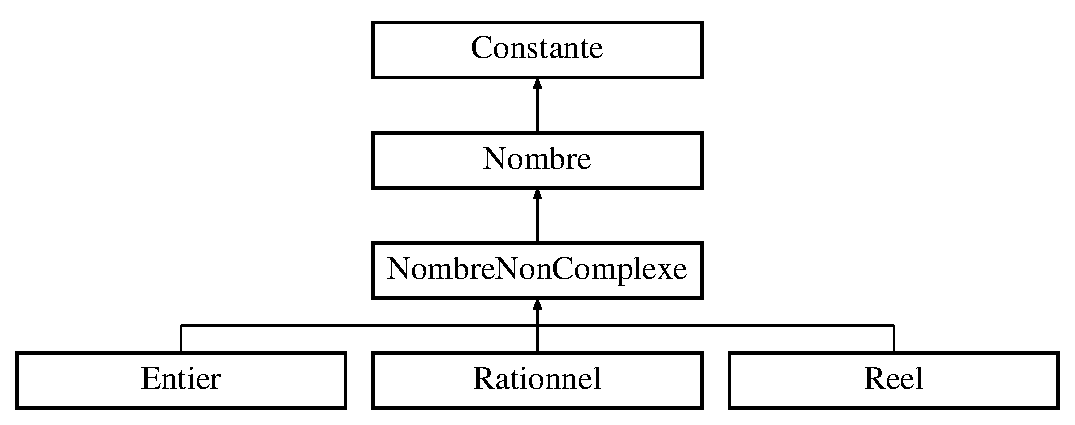
\includegraphics[height=4.000000cm]{class_nombre_non_complexe}
\end{center}
\end{figure}
\subsection*{Public Member Functions}
\begin{DoxyCompactItemize}
\item 
virtual \hyperlink{class_nombre_non_complexe_ad623268a2e87fb652342a984ccc70a7c}{$\sim$\-Nombre\-Non\-Complexe} ()
\begin{DoxyCompactList}\small\item\em Destructeur de l'instance de la classe \hyperlink{class_nombre_non_complexe}{Nombre\-Non\-Complexe}. \end{DoxyCompactList}\item 
\hyperlink{class_nombre_non_complexe}{Nombre\-Non\-Complexe} $\ast$ \hyperlink{class_nombre_non_complexe_a6081b502145e109bbed9d13a8685fead}{operator+} (\hyperlink{class_nombre_non_complexe}{Nombre\-Non\-Complexe} $\ast$nb)
\begin{DoxyCompactList}\small\item\em M�thode permettant de faire l'addition entre deux nombres. \end{DoxyCompactList}\item 
\hyperlink{class_nombre_non_complexe}{Nombre\-Non\-Complexe} $\ast$ \hyperlink{class_nombre_non_complexe_aeac1f3ad9a6e1e55690e1a28a4efa1e6}{operator-\/} (\hyperlink{class_nombre_non_complexe}{Nombre\-Non\-Complexe} $\ast$nb)
\begin{DoxyCompactList}\small\item\em M�thode permettant de faire la soustraction entre deux nombres. \end{DoxyCompactList}\item 
\hyperlink{class_nombre_non_complexe}{Nombre\-Non\-Complexe} $\ast$ \hyperlink{class_nombre_non_complexe_a73e31c766e28427c829514ffbaaf67ce}{operator/} (\hyperlink{class_nombre_non_complexe}{Nombre\-Non\-Complexe} $\ast$nb)
\begin{DoxyCompactList}\small\item\em M�thode permettant de faire la division entre deux nombres. \end{DoxyCompactList}\item 
\hyperlink{class_nombre_non_complexe}{Nombre\-Non\-Complexe} $\ast$ \hyperlink{class_nombre_non_complexe_a4ad5d4e68de267426a1d4d11bd079315}{operator$\ast$} (\hyperlink{class_nombre_non_complexe}{Nombre\-Non\-Complexe} $\ast$nb)
\begin{DoxyCompactList}\small\item\em M�thode permettant de faire la multiplication entre deux nombres. \end{DoxyCompactList}\item 
virtual \hyperlink{class_entier}{Entier} $\ast$ \hyperlink{class_nombre_non_complexe_a01370f18cfc8304cba476f21dab9f53c}{to\-Entier} ()
\begin{DoxyCompactList}\small\item\em M�thode permettant de convertir un \hyperlink{class_nombre_non_complexe}{Nombre\-Non\-Complexe} en son �quivalent \hyperlink{class_entier}{Entier}. \end{DoxyCompactList}\item 
virtual \hyperlink{class_rationnel}{Rationnel} $\ast$ \hyperlink{class_nombre_non_complexe_a9f4b8526b3c58d7c4a8531e15e08940e}{to\-Rationnel} ()
\begin{DoxyCompactList}\small\item\em M�thode permettant de convertir un \hyperlink{class_nombre_non_complexe}{Nombre\-Non\-Complexe} en son �quivalent \hyperlink{class_rationnel}{Rationnel}. \end{DoxyCompactList}\item 
virtual \hyperlink{class_reel}{Reel} $\ast$ \hyperlink{class_nombre_non_complexe_a6a573025d221b8fe3d85484a11bcffe0}{to\-Reel} ()
\begin{DoxyCompactList}\small\item\em M�thode permettant de convertir un \hyperlink{class_nombre_non_complexe}{Nombre\-Non\-Complexe} en son �quivalent \hyperlink{class_reel}{Reel}. \end{DoxyCompactList}\item 
virtual float \hyperlink{class_nombre_non_complexe_ad148f1e2a4626ecf279e91d04d1aff24}{get\-Float\-Val} () const =0
\begin{DoxyCompactList}\small\item\em M�thode permettant de r�cup�rer la valeur du \hyperlink{class_nombre_non_complexe}{Nombre\-Non\-Complexe} sous la forme d'un r�el. \end{DoxyCompactList}\item 
virtual void \hyperlink{class_nombre_non_complexe_a859175bae737e01e73316632f1083d07}{pow} (\hyperlink{class_entier}{Entier} $\ast$e)=0
\begin{DoxyCompactList}\small\item\em M�thode permettant d'effectuer la puissance d'un nombre. \end{DoxyCompactList}\end{DoxyCompactItemize}


\subsection{Detailed Description}
Classe qui �tend l'interface \hyperlink{class_nombre}{Nombre} et permettant de g�rer des constantes de type non complexe (\hyperlink{class_entier}{Entier}, \hyperlink{class_rationnel}{Rationnel}, \hyperlink{class_reel}{Reel}). 

Definition at line 23 of file nombre\-Non\-Complexe.\-h.



\subsection{Constructor \& Destructor Documentation}
\hypertarget{class_nombre_non_complexe_ad623268a2e87fb652342a984ccc70a7c}{\index{Nombre\-Non\-Complexe@{Nombre\-Non\-Complexe}!$\sim$\-Nombre\-Non\-Complexe@{$\sim$\-Nombre\-Non\-Complexe}}
\index{$\sim$\-Nombre\-Non\-Complexe@{$\sim$\-Nombre\-Non\-Complexe}!NombreNonComplexe@{Nombre\-Non\-Complexe}}
\subsubsection[{$\sim$\-Nombre\-Non\-Complexe}]{\setlength{\rightskip}{0pt plus 5cm}virtual {\bf Nombre\-Non\-Complexe\-::$\sim$\-Nombre\-Non\-Complexe} (
\begin{DoxyParamCaption}
{}
\end{DoxyParamCaption}
)\hspace{0.3cm}{\ttfamily  \mbox{[}inline, virtual\mbox{]}}}}\label{class_nombre_non_complexe_ad623268a2e87fb652342a984ccc70a7c}


Destructeur de l'instance de la classe \hyperlink{class_nombre_non_complexe}{Nombre\-Non\-Complexe}. 



Definition at line 29 of file nombre\-Non\-Complexe.\-h.



\subsection{Member Function Documentation}
\hypertarget{class_nombre_non_complexe_ad148f1e2a4626ecf279e91d04d1aff24}{\index{Nombre\-Non\-Complexe@{Nombre\-Non\-Complexe}!get\-Float\-Val@{get\-Float\-Val}}
\index{get\-Float\-Val@{get\-Float\-Val}!NombreNonComplexe@{Nombre\-Non\-Complexe}}
\subsubsection[{get\-Float\-Val}]{\setlength{\rightskip}{0pt plus 5cm}virtual float {\bf Nombre\-Non\-Complexe\-::get\-Float\-Val} (
\begin{DoxyParamCaption}
{}
\end{DoxyParamCaption}
) const\hspace{0.3cm}{\ttfamily  \mbox{[}pure virtual\mbox{]}}}}\label{class_nombre_non_complexe_ad148f1e2a4626ecf279e91d04d1aff24}


M�thode permettant de r�cup�rer la valeur du \hyperlink{class_nombre_non_complexe}{Nombre\-Non\-Complexe} sous la forme d'un r�el. 

\begin{DoxyReturn}{Returns}
La valeur r�elle 
\end{DoxyReturn}


Implemented in \hyperlink{class_rationnel_a026cd9c023e23034313140d592b6f38f}{Rationnel}, \hyperlink{class_entier_a4ce7f7cddbaa2a28d244444d18ef55dc}{Entier}, and \hyperlink{class_reel_a9d2e05f1f59ad433c3eafb2da7e09f86}{Reel}.

\hypertarget{class_nombre_non_complexe_a4ad5d4e68de267426a1d4d11bd079315}{\index{Nombre\-Non\-Complexe@{Nombre\-Non\-Complexe}!operator$\ast$@{operator$\ast$}}
\index{operator$\ast$@{operator$\ast$}!NombreNonComplexe@{Nombre\-Non\-Complexe}}
\subsubsection[{operator$\ast$}]{\setlength{\rightskip}{0pt plus 5cm}{\bf Nombre\-Non\-Complexe} $\ast$ Nombre\-Non\-Complexe\-::operator$\ast$ (
\begin{DoxyParamCaption}
\item[{{\bf Nombre\-Non\-Complexe} $\ast$}]{nb}
\end{DoxyParamCaption}
)}}\label{class_nombre_non_complexe_a4ad5d4e68de267426a1d4d11bd079315}


M�thode permettant de faire la multiplication entre deux nombres. 


\begin{DoxyParams}{Parameters}
{\em nb} & La deuxi�me op�rande \\
\hline
\end{DoxyParams}
\begin{DoxyReturn}{Returns}
Le produit des deux nombres 
\end{DoxyReturn}


Definition at line 52 of file nombre\-Non\-Complexe.\-cpp.

\hypertarget{class_nombre_non_complexe_a6081b502145e109bbed9d13a8685fead}{\index{Nombre\-Non\-Complexe@{Nombre\-Non\-Complexe}!operator+@{operator+}}
\index{operator+@{operator+}!NombreNonComplexe@{Nombre\-Non\-Complexe}}
\subsubsection[{operator+}]{\setlength{\rightskip}{0pt plus 5cm}{\bf Nombre\-Non\-Complexe} $\ast$ Nombre\-Non\-Complexe\-::operator+ (
\begin{DoxyParamCaption}
\item[{{\bf Nombre\-Non\-Complexe} $\ast$}]{nb}
\end{DoxyParamCaption}
)}}\label{class_nombre_non_complexe_a6081b502145e109bbed9d13a8685fead}


M�thode permettant de faire l'addition entre deux nombres. 


\begin{DoxyParams}{Parameters}
{\em nb} & La deuxi�me op�rande \\
\hline
\end{DoxyParams}
\begin{DoxyReturn}{Returns}
La somme des deux nombres 
\end{DoxyReturn}


Definition at line 8 of file nombre\-Non\-Complexe.\-cpp.

\hypertarget{class_nombre_non_complexe_aeac1f3ad9a6e1e55690e1a28a4efa1e6}{\index{Nombre\-Non\-Complexe@{Nombre\-Non\-Complexe}!operator-\/@{operator-\/}}
\index{operator-\/@{operator-\/}!NombreNonComplexe@{Nombre\-Non\-Complexe}}
\subsubsection[{operator-\/}]{\setlength{\rightskip}{0pt plus 5cm}{\bf Nombre\-Non\-Complexe} $\ast$ Nombre\-Non\-Complexe\-::operator-\/ (
\begin{DoxyParamCaption}
\item[{{\bf Nombre\-Non\-Complexe} $\ast$}]{nb}
\end{DoxyParamCaption}
)}}\label{class_nombre_non_complexe_aeac1f3ad9a6e1e55690e1a28a4efa1e6}


M�thode permettant de faire la soustraction entre deux nombres. 


\begin{DoxyParams}{Parameters}
{\em nb} & La deuxi�me op�rande \\
\hline
\end{DoxyParams}
\begin{DoxyReturn}{Returns}
La diff�rence entre les deux nombres 
\end{DoxyReturn}


Definition at line 20 of file nombre\-Non\-Complexe.\-cpp.

\hypertarget{class_nombre_non_complexe_a73e31c766e28427c829514ffbaaf67ce}{\index{Nombre\-Non\-Complexe@{Nombre\-Non\-Complexe}!operator/@{operator/}}
\index{operator/@{operator/}!NombreNonComplexe@{Nombre\-Non\-Complexe}}
\subsubsection[{operator/}]{\setlength{\rightskip}{0pt plus 5cm}{\bf Nombre\-Non\-Complexe} $\ast$ Nombre\-Non\-Complexe\-::operator/ (
\begin{DoxyParamCaption}
\item[{{\bf Nombre\-Non\-Complexe} $\ast$}]{nb}
\end{DoxyParamCaption}
)}}\label{class_nombre_non_complexe_a73e31c766e28427c829514ffbaaf67ce}


M�thode permettant de faire la division entre deux nombres. 


\begin{DoxyParams}{Parameters}
{\em nb} & La deuxi�me op�rande \\
\hline
\end{DoxyParams}
\begin{DoxyReturn}{Returns}
Le quotient de la division de ces deux nombres 
\end{DoxyReturn}


Definition at line 32 of file nombre\-Non\-Complexe.\-cpp.

\hypertarget{class_nombre_non_complexe_a859175bae737e01e73316632f1083d07}{\index{Nombre\-Non\-Complexe@{Nombre\-Non\-Complexe}!pow@{pow}}
\index{pow@{pow}!NombreNonComplexe@{Nombre\-Non\-Complexe}}
\subsubsection[{pow}]{\setlength{\rightskip}{0pt plus 5cm}virtual void {\bf Nombre\-Non\-Complexe\-::pow} (
\begin{DoxyParamCaption}
\item[{{\bf Entier} $\ast$}]{e}
\end{DoxyParamCaption}
)\hspace{0.3cm}{\ttfamily  \mbox{[}pure virtual\mbox{]}}}}\label{class_nombre_non_complexe_a859175bae737e01e73316632f1083d07}


M�thode permettant d'effectuer la puissance d'un nombre. 


\begin{DoxyParams}{Parameters}
{\em e} & Un entier correspondant � la puissance \\
\hline
\end{DoxyParams}


Implemented in \hyperlink{class_rationnel_a1d8ffa87d6fff2c6eade5e28533e5e78}{Rationnel}, \hyperlink{class_entier_ae44b026487bcd10fab16696eff3b49a8}{Entier}, and \hyperlink{class_reel_a11fda3f1bd3cdac610d3a2aeec2fc7ed}{Reel}.

\hypertarget{class_nombre_non_complexe_a01370f18cfc8304cba476f21dab9f53c}{\index{Nombre\-Non\-Complexe@{Nombre\-Non\-Complexe}!to\-Entier@{to\-Entier}}
\index{to\-Entier@{to\-Entier}!NombreNonComplexe@{Nombre\-Non\-Complexe}}
\subsubsection[{to\-Entier}]{\setlength{\rightskip}{0pt plus 5cm}{\bf Entier} $\ast$ {\bf Nombre\-Non\-Complexe\-::to\-Entier} (
\begin{DoxyParamCaption}
{}
\end{DoxyParamCaption}
)\hspace{0.3cm}{\ttfamily  \mbox{[}virtual\mbox{]}}}}\label{class_nombre_non_complexe_a01370f18cfc8304cba476f21dab9f53c}


M�thode permettant de convertir un \hyperlink{class_nombre_non_complexe}{Nombre\-Non\-Complexe} en son �quivalent \hyperlink{class_entier}{Entier}. 

\begin{DoxyReturn}{Returns}
Le pointeur vers l' \hyperlink{class_entier}{Entier} nouvellement cr�e 
\end{DoxyReturn}


Definition at line 61 of file nombre\-Non\-Complexe.\-cpp.

\hypertarget{class_nombre_non_complexe_a9f4b8526b3c58d7c4a8531e15e08940e}{\index{Nombre\-Non\-Complexe@{Nombre\-Non\-Complexe}!to\-Rationnel@{to\-Rationnel}}
\index{to\-Rationnel@{to\-Rationnel}!NombreNonComplexe@{Nombre\-Non\-Complexe}}
\subsubsection[{to\-Rationnel}]{\setlength{\rightskip}{0pt plus 5cm}{\bf Rationnel} $\ast$ {\bf Nombre\-Non\-Complexe\-::to\-Rationnel} (
\begin{DoxyParamCaption}
{}
\end{DoxyParamCaption}
)\hspace{0.3cm}{\ttfamily  \mbox{[}virtual\mbox{]}}}}\label{class_nombre_non_complexe_a9f4b8526b3c58d7c4a8531e15e08940e}


M�thode permettant de convertir un \hyperlink{class_nombre_non_complexe}{Nombre\-Non\-Complexe} en son �quivalent \hyperlink{class_rationnel}{Rationnel}. 

\begin{DoxyReturn}{Returns}
Le pointeur vers le \hyperlink{class_rationnel}{Rationnel} nouvellement cr�e 
\end{DoxyReturn}


Definition at line 76 of file nombre\-Non\-Complexe.\-cpp.

\hypertarget{class_nombre_non_complexe_a6a573025d221b8fe3d85484a11bcffe0}{\index{Nombre\-Non\-Complexe@{Nombre\-Non\-Complexe}!to\-Reel@{to\-Reel}}
\index{to\-Reel@{to\-Reel}!NombreNonComplexe@{Nombre\-Non\-Complexe}}
\subsubsection[{to\-Reel}]{\setlength{\rightskip}{0pt plus 5cm}{\bf Reel} $\ast$ {\bf Nombre\-Non\-Complexe\-::to\-Reel} (
\begin{DoxyParamCaption}
{}
\end{DoxyParamCaption}
)\hspace{0.3cm}{\ttfamily  \mbox{[}virtual\mbox{]}}}}\label{class_nombre_non_complexe_a6a573025d221b8fe3d85484a11bcffe0}


M�thode permettant de convertir un \hyperlink{class_nombre_non_complexe}{Nombre\-Non\-Complexe} en son �quivalent \hyperlink{class_reel}{Reel}. 

\begin{DoxyReturn}{Returns}
Le pointeur vers le \hyperlink{class_reel}{Reel} nouvellement cr�e 
\end{DoxyReturn}


Definition at line 91 of file nombre\-Non\-Complexe.\-cpp.



The documentation for this class was generated from the following files\-:\begin{DoxyCompactItemize}
\item 
\hyperlink{nombre_non_complexe_8h}{nombre\-Non\-Complexe.\-h}\item 
\hyperlink{nombre_non_complexe_8cpp}{nombre\-Non\-Complexe.\-cpp}\end{DoxyCompactItemize}

\hypertarget{class_operateur}{\section{Operateur Class Reference}
\label{class_operateur}\index{Operateur@{Operateur}}
}


Classe (utilisant le design pattern strategy) impl�mentant l'interface de \hyperlink{class_constante}{Constante} et permettant de g�rer les constantes de type op�rateur (+,-\/,/,$\ast$, sin, cos, etc...).  




{\ttfamily \#include $<$operateur.\-h$>$}

Inheritance diagram for Operateur\-:\begin{figure}[H]
\begin{center}
\leavevmode
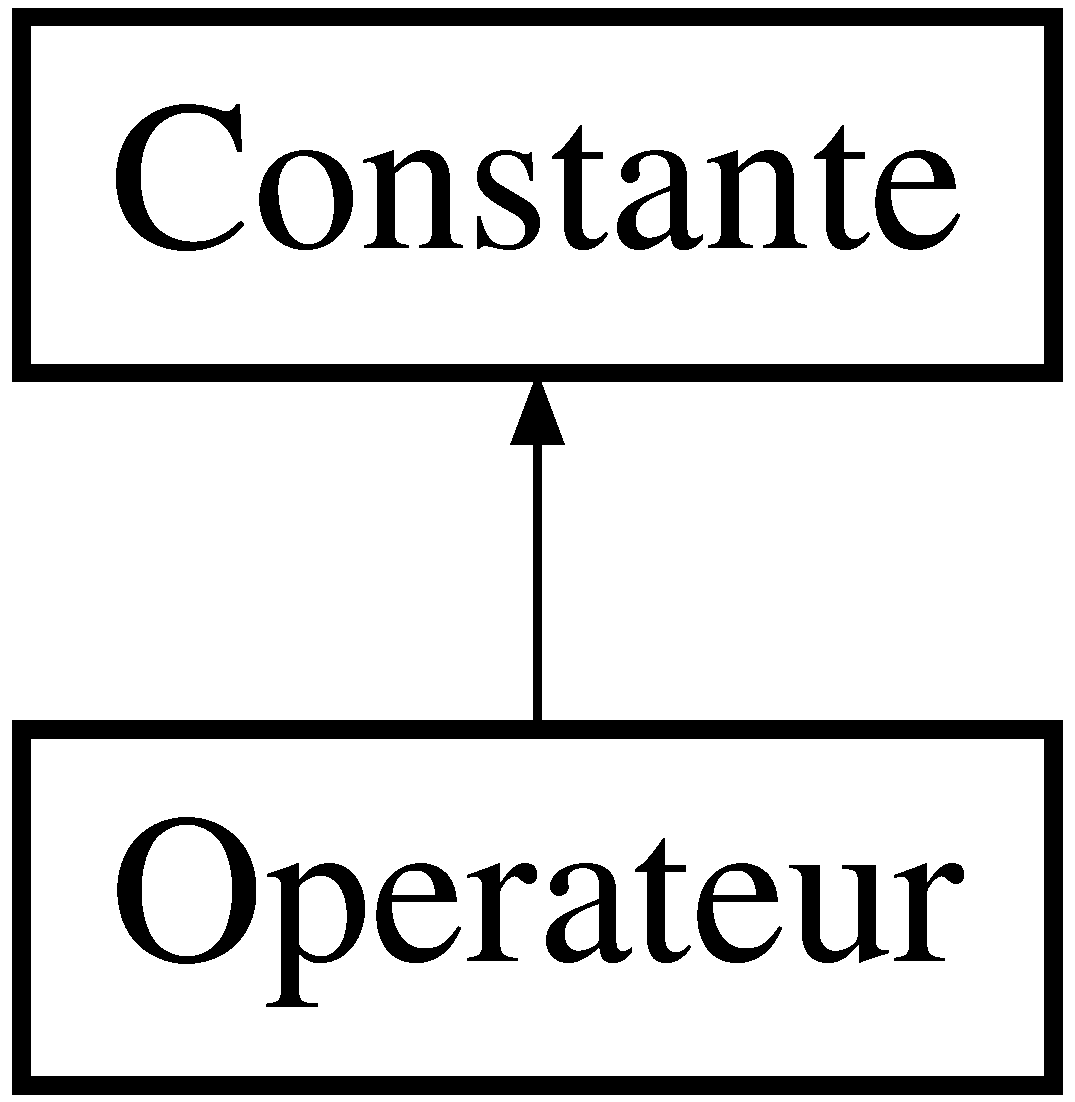
\includegraphics[height=2.000000cm]{class_operateur}
\end{center}
\end{figure}
\subsection*{Public Member Functions}
\begin{DoxyCompactItemize}
\item 
\hyperlink{class_operateur_a94687115012fbac2cb9b3019bf613398}{Operateur} ()
\begin{DoxyCompactList}\small\item\em Constructeur par d�faut. \end{DoxyCompactList}\item 
\hyperlink{class_operateur_a3c456363e365eb379607da810738482d}{Operateur} (const Q\-String \&op, int ar)
\begin{DoxyCompactList}\small\item\em Constructeur avec param�tres. \end{DoxyCompactList}\item 
\hyperlink{class_operateur}{Operateur} $\ast$ \hyperlink{class_operateur_a77814d91250ee0c65501cea7d135b76c}{clone} () const 
\begin{DoxyCompactList}\small\item\em M�thode permettant de cloner une constante.  \end{DoxyCompactList}\item 
Q\-String \hyperlink{class_operateur_afdae3d8564054da4d8a8a05efa86a172}{get\-Operateur} () const 
\begin{DoxyCompactList}\small\item\em Getter de la chaine representant l'operateur. \end{DoxyCompactList}\item 
int \hyperlink{class_operateur_a91dfb13c9feb888dc50873ed53cae210}{get\-Arite} () const 
\begin{DoxyCompactList}\small\item\em Getter de l'int representant l'arit� \end{DoxyCompactList}\item 
Q\-String \hyperlink{class_operateur_ad49ae9c67adcd3af3a9be0e2bc13c629}{to\-String} () const 
\begin{DoxyCompactList}\small\item\em Fonction permettant de renvoyer une chaine comprenant la valuation de la constante associ�, cette fonction est utilis�e dans le cadre de l'affichage des constantes dans la pile.  \end{DoxyCompactList}\item 
\hyperlink{class_constante}{Constante} $\ast$ \hyperlink{class_operateur_a8e517c5d95b239024d8d757d4e79ddf2}{call} (\hyperlink{class_constante}{Constante} $\ast$c1=0, \hyperlink{class_constante}{Constante} $\ast$c2=0)
\begin{DoxyCompactList}\small\item\em M�thode permettant d'appeler la bonne m�thode en fonction de l'op�rateur et des deux constantes associ�es. \end{DoxyCompactList}\end{DoxyCompactItemize}


\subsection{Detailed Description}
Classe (utilisant le design pattern strategy) impl�mentant l'interface de \hyperlink{class_constante}{Constante} et permettant de g�rer les constantes de type op�rateur (+,-\/,/,$\ast$, sin, cos, etc...). 

Definition at line 18 of file operateur.\-h.



\subsection{Constructor \& Destructor Documentation}
\hypertarget{class_operateur_a94687115012fbac2cb9b3019bf613398}{\index{Operateur@{Operateur}!Operateur@{Operateur}}
\index{Operateur@{Operateur}!Operateur@{Operateur}}
\subsubsection[{Operateur}]{\setlength{\rightskip}{0pt plus 5cm}{\bf Operateur\-::\-Operateur} (
\begin{DoxyParamCaption}
{}
\end{DoxyParamCaption}
)}}\label{class_operateur_a94687115012fbac2cb9b3019bf613398}


Constructeur par d�faut. 

\hypertarget{class_operateur_a3c456363e365eb379607da810738482d}{\index{Operateur@{Operateur}!Operateur@{Operateur}}
\index{Operateur@{Operateur}!Operateur@{Operateur}}
\subsubsection[{Operateur}]{\setlength{\rightskip}{0pt plus 5cm}{\bf Operateur\-::\-Operateur} (
\begin{DoxyParamCaption}
\item[{const Q\-String \&}]{op, }
\item[{int}]{ar}
\end{DoxyParamCaption}
)\hspace{0.3cm}{\ttfamily  \mbox{[}inline\mbox{]}}}}\label{class_operateur_a3c456363e365eb379607da810738482d}


Constructeur avec param�tres. 


\begin{DoxyParams}{Parameters}
{\em op} & La chaine repr�sentant l'op�rateur \\
\hline
{\em ar} & L'arit� de l'op�rateur \\
\hline
\end{DoxyParams}


Definition at line 38 of file operateur.\-h.



\subsection{Member Function Documentation}
\hypertarget{class_operateur_a8e517c5d95b239024d8d757d4e79ddf2}{\index{Operateur@{Operateur}!call@{call}}
\index{call@{call}!Operateur@{Operateur}}
\subsubsection[{call}]{\setlength{\rightskip}{0pt plus 5cm}{\bf Constante} $\ast$ {\bf Operateur\-::call} (
\begin{DoxyParamCaption}
\item[{{\bf Constante} $\ast$}]{c1 = {\ttfamily 0}, }
\item[{{\bf Constante} $\ast$}]{c2 = {\ttfamily 0}}
\end{DoxyParamCaption}
)}}\label{class_operateur_a8e517c5d95b239024d8d757d4e79ddf2}


M�thode permettant d'appeler la bonne m�thode en fonction de l'op�rateur et des deux constantes associ�es. 


\begin{DoxyParams}{Parameters}
{\em c1} & La premi�re op�rande (pr�sente dans le cas d'une op�ration unaire \& binaire) \\
\hline
{\em c2} & La seconde op�rande (pr�sente dans le cas d'une op�ration binaire) \\
\hline
\end{DoxyParams}
\begin{DoxyReturn}{Returns}
Le r�sultat de type \hyperlink{class_constante}{Constante} apr�s avoir appliqu� l'op�ration 
\end{DoxyReturn}


Definition at line 17 of file operateur.\-cpp.

\hypertarget{class_operateur_a77814d91250ee0c65501cea7d135b76c}{\index{Operateur@{Operateur}!clone@{clone}}
\index{clone@{clone}!Operateur@{Operateur}}
\subsubsection[{clone}]{\setlength{\rightskip}{0pt plus 5cm}{\bf Operateur} $\ast$ {\bf Operateur\-::clone} (
\begin{DoxyParamCaption}
{}
\end{DoxyParamCaption}
) const\hspace{0.3cm}{\ttfamily  \mbox{[}virtual\mbox{]}}}}\label{class_operateur_a77814d91250ee0c65501cea7d135b76c}


M�thode permettant de cloner une constante.  


\begin{DoxyParams}{Parameters}
{\em Le} & pointeur vers la constante clon�e \\
\hline
\end{DoxyParams}
 

Implements \hyperlink{class_constante_a5769ea385161e02bd2d1bcadefc2c510}{Constante}.



Definition at line 13 of file operateur.\-cpp.

\hypertarget{class_operateur_a91dfb13c9feb888dc50873ed53cae210}{\index{Operateur@{Operateur}!get\-Arite@{get\-Arite}}
\index{get\-Arite@{get\-Arite}!Operateur@{Operateur}}
\subsubsection[{get\-Arite}]{\setlength{\rightskip}{0pt plus 5cm}int {\bf Operateur\-::get\-Arite} (
\begin{DoxyParamCaption}
{}
\end{DoxyParamCaption}
) const\hspace{0.3cm}{\ttfamily  \mbox{[}inline\mbox{]}}}}\label{class_operateur_a91dfb13c9feb888dc50873ed53cae210}


Getter de l'int representant l'arit� 

\begin{DoxyReturn}{Returns}
L'arit� de l'op�rateur 
\end{DoxyReturn}


Definition at line 52 of file operateur.\-h.

\hypertarget{class_operateur_afdae3d8564054da4d8a8a05efa86a172}{\index{Operateur@{Operateur}!get\-Operateur@{get\-Operateur}}
\index{get\-Operateur@{get\-Operateur}!Operateur@{Operateur}}
\subsubsection[{get\-Operateur}]{\setlength{\rightskip}{0pt plus 5cm}Q\-String {\bf Operateur\-::get\-Operateur} (
\begin{DoxyParamCaption}
{}
\end{DoxyParamCaption}
) const\hspace{0.3cm}{\ttfamily  \mbox{[}inline\mbox{]}}}}\label{class_operateur_afdae3d8564054da4d8a8a05efa86a172}


Getter de la chaine representant l'operateur. 

\begin{DoxyReturn}{Returns}
La chaine correspondant � l'op�rateur 
\end{DoxyReturn}


Definition at line 47 of file operateur.\-h.

\hypertarget{class_operateur_ad49ae9c67adcd3af3a9be0e2bc13c629}{\index{Operateur@{Operateur}!to\-String@{to\-String}}
\index{to\-String@{to\-String}!Operateur@{Operateur}}
\subsubsection[{to\-String}]{\setlength{\rightskip}{0pt plus 5cm}Q\-String {\bf Operateur\-::to\-String} (
\begin{DoxyParamCaption}
{}
\end{DoxyParamCaption}
) const\hspace{0.3cm}{\ttfamily  \mbox{[}inline, virtual\mbox{]}}}}\label{class_operateur_ad49ae9c67adcd3af3a9be0e2bc13c629}


Fonction permettant de renvoyer une chaine comprenant la valuation de la constante associ�, cette fonction est utilis�e dans le cadre de l'affichage des constantes dans la pile.  

\begin{DoxyReturn}{Returns}
La chaine � afficher dans la pile 
\end{DoxyReturn}
 

Implements \hyperlink{class_constante_ad5ea6850196ee9f86b74c74009a87ab1}{Constante}.



Definition at line 56 of file operateur.\-h.



The documentation for this class was generated from the following files\-:\begin{DoxyCompactItemize}
\item 
\hyperlink{operateur_8h}{operateur.\-h}\item 
\hyperlink{operateur_8cpp}{operateur.\-cpp}\end{DoxyCompactItemize}

\hypertarget{class_pile}{\section{Pile Class Reference}
\label{class_pile}\index{Pile@{Pile}}
}


Classe permettant de g�rer la pile d'�l�ments et �galement l'historique de cette pile.  




{\ttfamily \#include $<$pile.\-h$>$}

\subsection*{Public Member Functions}
\begin{DoxyCompactItemize}
\item 
\hyperlink{class_pile_ab44e927107b28f5f3ac7697d10e0a739}{Pile} ()
\begin{DoxyCompactList}\small\item\em Initialise la pile avec des valeurs par d�fauts. \end{DoxyCompactList}\item 
\hyperlink{class_pile_ab2d1398d675586ff34994e2b109df152}{$\sim$\-Pile} ()
\begin{DoxyCompactList}\small\item\em Destructeur de la \hyperlink{class_pile}{Pile}. \end{DoxyCompactList}\item 
void \hyperlink{class_pile_a1bf6eb327e81b7eab70c0d3699a11d44}{push} (\hyperlink{class_constante}{Constante} $\ast$constante)
\begin{DoxyCompactList}\small\item\em M�thode permettant d'ajouter un �l�ment � la liste. \end{DoxyCompactList}\item 
\hyperlink{class_constante}{Constante} $\ast$ \hyperlink{class_pile_a2bbdc329f485cd017f8cbf88456ae68a}{pop} ()  throw (\-Log\-Message)
\begin{DoxyCompactList}\small\item\em M�thode permettant d'enlever un �l�ment de la liste et de la renvoyer. \end{DoxyCompactList}\item 
\hyperlink{class_constante}{Constante} $\ast$ \hyperlink{class_pile_ab379695209bed07fbcd9d2ca6ee6cf84}{sommet} ()
\begin{DoxyCompactList}\small\item\em M�thode permettant de retourner le sommet de la pile. \end{DoxyCompactList}\item 
Q\-String \hyperlink{class_pile_ad6dfffef3f69d3e51177ed9c5086907c}{get\-Pile\-String} () const 
\begin{DoxyCompactList}\small\item\em M�thode permettant de retourner une Q\-Strinf repr�sentant tout les �l�ments mis bout � bout, cette m�thode est notamment utilis� dans la classe \hyperlink{}{Contexte}. \end{DoxyCompactList}\item 
int \hyperlink{class_pile_a9dc49f9322d3869843843d4a4fd13a5e}{get\-Pile\-Affichage\-Size} () const 
\begin{DoxyCompactList}\small\item\em M�thode permettant de r�cup�rer la taille de la pile contenant les \hyperlink{class_constante}{Constante}. \end{DoxyCompactList}\item 
void \hyperlink{class_pile_ab1af47a73ec38e317baca0263ba58365}{set\-Nb\-Elem\-Affichable} (int i)
\begin{DoxyCompactList}\small\item\em M�thode permettant de d�finir le nombre de \hyperlink{class_constante}{Constante} qui seront affich�es dans la pile d'affichage. \end{DoxyCompactList}\item 
void \hyperlink{class_pile_abcfa651f8ef3f2b42ecbbfc8e23b1cbd}{ajoute\-Historique} (\hyperlink{class_historique}{Historique} $\ast$e)
\begin{DoxyCompactList}\small\item\em M�thode permettant d'ajouter un nouvel �l�ment de type \hyperlink{class_historique}{Historique} dans la liste des historiques. \end{DoxyCompactList}\item 
void \hyperlink{class_pile_a7488ed257c6ceb16ed57a9fffb0726d5}{drop} ()
\begin{DoxyCompactList}\small\item\em M�thode permettant de supprimer le dernier �l�ment ins�rer dans la pile. \end{DoxyCompactList}\item 
void \hyperlink{class_pile_aa3991438f190580607d7bbbd50ecc0c3}{clear} ()
\begin{DoxyCompactList}\small\item\em M�thode permettant de nettoyer tout les �l�ments de la pile. \end{DoxyCompactList}\item 
void \hyperlink{class_pile_a081f7843d01cae1f0f7be7d92e46d5d2}{dup} ()
\begin{DoxyCompactList}\small\item\em M�thode permettant de dupliquer le sommet de la pile. \end{DoxyCompactList}\item 
void \hyperlink{class_pile_a1a19ce2a4a6a76286fae8243a1f9e247}{swap} (int x, int y)
\begin{DoxyCompactList}\small\item\em M�thode permettant d'�changer l'ordre de deux �l�ments de la pile. \end{DoxyCompactList}\item 
void \hyperlink{class_pile_ae09e2cf01c21b58a6c2c4efee101c158}{sum} (int x)
\begin{DoxyCompactList}\small\item\em M�thode permettant de faire la somme des x premiers �l�ments de la pile. \end{DoxyCompactList}\item 
void \hyperlink{class_pile_a1daebba5bd1d6c6d79de63728cc892a9}{mean} (int x)
\begin{DoxyCompactList}\small\item\em M�thode permettant de faire la moyenne des x premiers �l�ments de la pile. \end{DoxyCompactList}\item 
void \hyperlink{class_pile_aa8319a2921d86236d135cff700a5f833}{redo} ()
\begin{DoxyCompactList}\small\item\em M�thode permettant de r�tablir la derniere op�ration qui a �t� annul�e. \end{DoxyCompactList}\item 
void \hyperlink{class_pile_af91a4b277236024aa5aab9ef410881bb}{undo} ()
\begin{DoxyCompactList}\small\item\em M�thode permettant d'annuler la derniere op�ration qui a �t� effectu�e. \end{DoxyCompactList}\item 
void \hyperlink{class_pile_aed9e5c3126ffdde3b35217f8235df938}{affiche} ()
\begin{DoxyCompactList}\small\item\em M�thode permettant d'afficher les �l�ments contenus dans la pile dans l'interface graphique. \end{DoxyCompactList}\end{DoxyCompactItemize}


\subsection{Detailed Description}
Classe permettant de g�rer la pile d'�l�ments et �galement l'historique de cette pile. 

Definition at line 20 of file pile.\-h.



\subsection{Constructor \& Destructor Documentation}
\hypertarget{class_pile_ab44e927107b28f5f3ac7697d10e0a739}{\index{Pile@{Pile}!Pile@{Pile}}
\index{Pile@{Pile}!Pile@{Pile}}
\subsubsection[{Pile}]{\setlength{\rightskip}{0pt plus 5cm}{\bf Pile\-::\-Pile} (
\begin{DoxyParamCaption}
{}
\end{DoxyParamCaption}
)}}\label{class_pile_ab44e927107b28f5f3ac7697d10e0a739}


Initialise la pile avec des valeurs par d�fauts. 



Definition at line 9 of file pile.\-cpp.

\hypertarget{class_pile_ab2d1398d675586ff34994e2b109df152}{\index{Pile@{Pile}!$\sim$\-Pile@{$\sim$\-Pile}}
\index{$\sim$\-Pile@{$\sim$\-Pile}!Pile@{Pile}}
\subsubsection[{$\sim$\-Pile}]{\setlength{\rightskip}{0pt plus 5cm}{\bf Pile\-::$\sim$\-Pile} (
\begin{DoxyParamCaption}
{}
\end{DoxyParamCaption}
)}}\label{class_pile_ab2d1398d675586ff34994e2b109df152}


Destructeur de la \hyperlink{class_pile}{Pile}. 



Definition at line 17 of file pile.\-cpp.



\subsection{Member Function Documentation}
\hypertarget{class_pile_aed9e5c3126ffdde3b35217f8235df938}{\index{Pile@{Pile}!affiche@{affiche}}
\index{affiche@{affiche}!Pile@{Pile}}
\subsubsection[{affiche}]{\setlength{\rightskip}{0pt plus 5cm}void {\bf Pile\-::affiche} (
\begin{DoxyParamCaption}
{}
\end{DoxyParamCaption}
)}}\label{class_pile_aed9e5c3126ffdde3b35217f8235df938}


M�thode permettant d'afficher les �l�ments contenus dans la pile dans l'interface graphique. 



Definition at line 152 of file pile.\-cpp.

\hypertarget{class_pile_abcfa651f8ef3f2b42ecbbfc8e23b1cbd}{\index{Pile@{Pile}!ajoute\-Historique@{ajoute\-Historique}}
\index{ajoute\-Historique@{ajoute\-Historique}!Pile@{Pile}}
\subsubsection[{ajoute\-Historique}]{\setlength{\rightskip}{0pt plus 5cm}void {\bf Pile\-::ajoute\-Historique} (
\begin{DoxyParamCaption}
\item[{{\bf Historique} $\ast$}]{e}
\end{DoxyParamCaption}
)\hspace{0.3cm}{\ttfamily  \mbox{[}inline\mbox{]}}}}\label{class_pile_abcfa651f8ef3f2b42ecbbfc8e23b1cbd}


M�thode permettant d'ajouter un nouvel �l�ment de type \hyperlink{class_historique}{Historique} dans la liste des historiques. 


\begin{DoxyParams}{Parameters}
{\em e} & L'�lement de type \hyperlink{class_historique}{Historique} � ajouter \\
\hline
\end{DoxyParams}


Definition at line 84 of file pile.\-h.

\hypertarget{class_pile_aa3991438f190580607d7bbbd50ecc0c3}{\index{Pile@{Pile}!clear@{clear}}
\index{clear@{clear}!Pile@{Pile}}
\subsubsection[{clear}]{\setlength{\rightskip}{0pt plus 5cm}void {\bf Pile\-::clear} (
\begin{DoxyParamCaption}
{}
\end{DoxyParamCaption}
)}}\label{class_pile_aa3991438f190580607d7bbbd50ecc0c3}


M�thode permettant de nettoyer tout les �l�ments de la pile. 



Definition at line 28 of file pile.\-cpp.

\hypertarget{class_pile_a7488ed257c6ceb16ed57a9fffb0726d5}{\index{Pile@{Pile}!drop@{drop}}
\index{drop@{drop}!Pile@{Pile}}
\subsubsection[{drop}]{\setlength{\rightskip}{0pt plus 5cm}void {\bf Pile\-::drop} (
\begin{DoxyParamCaption}
{}
\end{DoxyParamCaption}
)}}\label{class_pile_a7488ed257c6ceb16ed57a9fffb0726d5}


M�thode permettant de supprimer le dernier �l�ment ins�rer dans la pile. 



Definition at line 33 of file pile.\-cpp.

\hypertarget{class_pile_a081f7843d01cae1f0f7be7d92e46d5d2}{\index{Pile@{Pile}!dup@{dup}}
\index{dup@{dup}!Pile@{Pile}}
\subsubsection[{dup}]{\setlength{\rightskip}{0pt plus 5cm}void {\bf Pile\-::dup} (
\begin{DoxyParamCaption}
{}
\end{DoxyParamCaption}
)}}\label{class_pile_a081f7843d01cae1f0f7be7d92e46d5d2}


M�thode permettant de dupliquer le sommet de la pile. 



Definition at line 39 of file pile.\-cpp.

\hypertarget{class_pile_a9dc49f9322d3869843843d4a4fd13a5e}{\index{Pile@{Pile}!get\-Pile\-Affichage\-Size@{get\-Pile\-Affichage\-Size}}
\index{get\-Pile\-Affichage\-Size@{get\-Pile\-Affichage\-Size}!Pile@{Pile}}
\subsubsection[{get\-Pile\-Affichage\-Size}]{\setlength{\rightskip}{0pt plus 5cm}int {\bf Pile\-::get\-Pile\-Affichage\-Size} (
\begin{DoxyParamCaption}
{}
\end{DoxyParamCaption}
) const\hspace{0.3cm}{\ttfamily  \mbox{[}inline\mbox{]}}}}\label{class_pile_a9dc49f9322d3869843843d4a4fd13a5e}


M�thode permettant de r�cup�rer la taille de la pile contenant les \hyperlink{class_constante}{Constante}. 

\begin{DoxyReturn}{Returns}
La taille de la pile 
\end{DoxyReturn}


Definition at line 74 of file pile.\-h.

\hypertarget{class_pile_ad6dfffef3f69d3e51177ed9c5086907c}{\index{Pile@{Pile}!get\-Pile\-String@{get\-Pile\-String}}
\index{get\-Pile\-String@{get\-Pile\-String}!Pile@{Pile}}
\subsubsection[{get\-Pile\-String}]{\setlength{\rightskip}{0pt plus 5cm}Q\-String {\bf Pile\-::get\-Pile\-String} (
\begin{DoxyParamCaption}
{}
\end{DoxyParamCaption}
) const}}\label{class_pile_ad6dfffef3f69d3e51177ed9c5086907c}


M�thode permettant de retourner une Q\-Strinf repr�sentant tout les �l�ments mis bout � bout, cette m�thode est notamment utilis� dans la classe \hyperlink{}{Contexte}. 



Definition at line 166 of file pile.\-cpp.

\hypertarget{class_pile_a1daebba5bd1d6c6d79de63728cc892a9}{\index{Pile@{Pile}!mean@{mean}}
\index{mean@{mean}!Pile@{Pile}}
\subsubsection[{mean}]{\setlength{\rightskip}{0pt plus 5cm}void {\bf Pile\-::mean} (
\begin{DoxyParamCaption}
\item[{int}]{x}
\end{DoxyParamCaption}
)}}\label{class_pile_a1daebba5bd1d6c6d79de63728cc892a9}


M�thode permettant de faire la moyenne des x premiers �l�ments de la pile. 


\begin{DoxyParams}{Parameters}
{\em x} & Le nombre d'�l�ments \\
\hline
\end{DoxyParams}


Definition at line 48 of file pile.\-cpp.

\hypertarget{class_pile_a2bbdc329f485cd017f8cbf88456ae68a}{\index{Pile@{Pile}!pop@{pop}}
\index{pop@{pop}!Pile@{Pile}}
\subsubsection[{pop}]{\setlength{\rightskip}{0pt plus 5cm}{\bf Constante} $\ast$ {\bf Pile\-::pop} (
\begin{DoxyParamCaption}
{}
\end{DoxyParamCaption}
)  throw ({\bf Log\-Message})}}\label{class_pile_a2bbdc329f485cd017f8cbf88456ae68a}


M�thode permettant d'enlever un �l�ment de la liste et de la renvoyer. 

\begin{DoxyReturn}{Returns}
La constante enlev�e de la liste 
\end{DoxyReturn}


Definition at line 138 of file pile.\-cpp.

\hypertarget{class_pile_a1bf6eb327e81b7eab70c0d3699a11d44}{\index{Pile@{Pile}!push@{push}}
\index{push@{push}!Pile@{Pile}}
\subsubsection[{push}]{\setlength{\rightskip}{0pt plus 5cm}void {\bf Pile\-::push} (
\begin{DoxyParamCaption}
\item[{{\bf Constante} $\ast$}]{constante}
\end{DoxyParamCaption}
)}}\label{class_pile_a1bf6eb327e81b7eab70c0d3699a11d44}


M�thode permettant d'ajouter un �l�ment � la liste. 


\begin{DoxyParams}{Parameters}
{\em constante} & La constante � ajouter � la liste \\
\hline
\end{DoxyParams}


Definition at line 147 of file pile.\-cpp.

\hypertarget{class_pile_aa8319a2921d86236d135cff700a5f833}{\index{Pile@{Pile}!redo@{redo}}
\index{redo@{redo}!Pile@{Pile}}
\subsubsection[{redo}]{\setlength{\rightskip}{0pt plus 5cm}void {\bf Pile\-::redo} (
\begin{DoxyParamCaption}
{}
\end{DoxyParamCaption}
)}}\label{class_pile_aa8319a2921d86236d135cff700a5f833}


M�thode permettant de r�tablir la derniere op�ration qui a �t� annul�e. 



Definition at line 110 of file pile.\-cpp.

\hypertarget{class_pile_ab1af47a73ec38e317baca0263ba58365}{\index{Pile@{Pile}!set\-Nb\-Elem\-Affichable@{set\-Nb\-Elem\-Affichable}}
\index{set\-Nb\-Elem\-Affichable@{set\-Nb\-Elem\-Affichable}!Pile@{Pile}}
\subsubsection[{set\-Nb\-Elem\-Affichable}]{\setlength{\rightskip}{0pt plus 5cm}void {\bf Pile\-::set\-Nb\-Elem\-Affichable} (
\begin{DoxyParamCaption}
\item[{int}]{i}
\end{DoxyParamCaption}
)\hspace{0.3cm}{\ttfamily  \mbox{[}inline\mbox{]}}}}\label{class_pile_ab1af47a73ec38e317baca0263ba58365}


M�thode permettant de d�finir le nombre de \hyperlink{class_constante}{Constante} qui seront affich�es dans la pile d'affichage. 


\begin{DoxyParams}{Parameters}
{\em i} & Le nombre d'�l�ment que l'on veut afficher \\
\hline
\end{DoxyParams}


Definition at line 79 of file pile.\-h.

\hypertarget{class_pile_ab379695209bed07fbcd9d2ca6ee6cf84}{\index{Pile@{Pile}!sommet@{sommet}}
\index{sommet@{sommet}!Pile@{Pile}}
\subsubsection[{sommet}]{\setlength{\rightskip}{0pt plus 5cm}{\bf Constante} $\ast$ {\bf Pile\-::sommet} (
\begin{DoxyParamCaption}
{}
\end{DoxyParamCaption}
)}}\label{class_pile_ab379695209bed07fbcd9d2ca6ee6cf84}


M�thode permettant de retourner le sommet de la pile. 

\begin{DoxyReturn}{Returns}
Le sommet de la pile de type \hyperlink{class_constante}{Constante} 
\end{DoxyReturn}


Definition at line 130 of file pile.\-cpp.

\hypertarget{class_pile_ae09e2cf01c21b58a6c2c4efee101c158}{\index{Pile@{Pile}!sum@{sum}}
\index{sum@{sum}!Pile@{Pile}}
\subsubsection[{sum}]{\setlength{\rightskip}{0pt plus 5cm}void {\bf Pile\-::sum} (
\begin{DoxyParamCaption}
\item[{int}]{x}
\end{DoxyParamCaption}
)}}\label{class_pile_ae09e2cf01c21b58a6c2c4efee101c158}


M�thode permettant de faire la somme des x premiers �l�ments de la pile. 


\begin{DoxyParams}{Parameters}
{\em x} & Le nombre d'�l�ments \\
\hline
\end{DoxyParams}


Definition at line 78 of file pile.\-cpp.

\hypertarget{class_pile_a1a19ce2a4a6a76286fae8243a1f9e247}{\index{Pile@{Pile}!swap@{swap}}
\index{swap@{swap}!Pile@{Pile}}
\subsubsection[{swap}]{\setlength{\rightskip}{0pt plus 5cm}void {\bf Pile\-::swap} (
\begin{DoxyParamCaption}
\item[{int}]{x, }
\item[{int}]{y}
\end{DoxyParamCaption}
)}}\label{class_pile_a1a19ce2a4a6a76286fae8243a1f9e247}


M�thode permettant d'�changer l'ordre de deux �l�ments de la pile. 


\begin{DoxyParams}{Parameters}
{\em x} & L'indice du premier �l�ment \\
\hline
{\em y} & L'indice du deuxi�me �l�ment \\
\hline
\end{DoxyParams}


Definition at line 100 of file pile.\-cpp.

\hypertarget{class_pile_af91a4b277236024aa5aab9ef410881bb}{\index{Pile@{Pile}!undo@{undo}}
\index{undo@{undo}!Pile@{Pile}}
\subsubsection[{undo}]{\setlength{\rightskip}{0pt plus 5cm}void {\bf Pile\-::undo} (
\begin{DoxyParamCaption}
{}
\end{DoxyParamCaption}
)}}\label{class_pile_af91a4b277236024aa5aab9ef410881bb}


M�thode permettant d'annuler la derniere op�ration qui a �t� effectu�e. 



Definition at line 120 of file pile.\-cpp.



The documentation for this class was generated from the following files\-:\begin{DoxyCompactItemize}
\item 
\hyperlink{pile_8h}{pile.\-h}\item 
\hyperlink{pile_8cpp}{pile.\-cpp}\end{DoxyCompactItemize}

\hypertarget{class_rationnel}{\section{Rationnel Class Reference}
\label{class_rationnel}\index{Rationnel@{Rationnel}}
}


Classe impl�mentant l'interface de \hyperlink{class_nombre_non_complexe}{Nombre\-Non\-Complexe} et permettant de g�rer les constantes de type rationnel.  




{\ttfamily \#include $<$rationnel.\-h$>$}

Inheritance diagram for Rationnel\-:\begin{figure}[H]
\begin{center}
\leavevmode
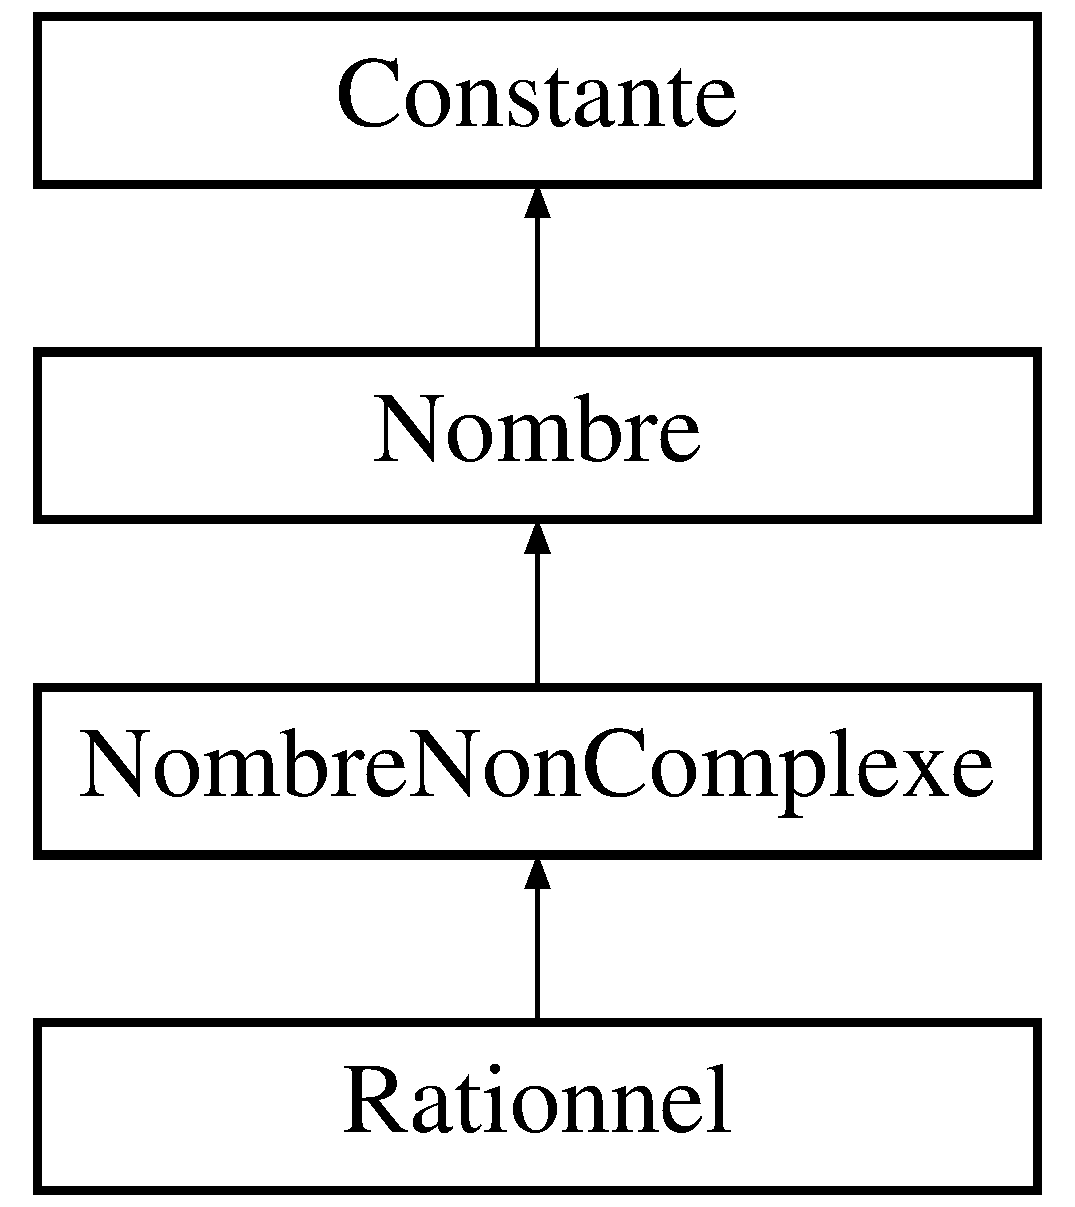
\includegraphics[height=4.000000cm]{class_rationnel}
\end{center}
\end{figure}
\subsection*{Public Member Functions}
\begin{DoxyCompactItemize}
\item 
\hyperlink{class_rationnel_ab0257aa2fd1b258506ec6d2a268612c6}{$\sim$\-Rationnel} ()
\begin{DoxyCompactList}\small\item\em Destructeur de la classe. \end{DoxyCompactList}\item 
\hyperlink{class_rationnel_a9adcf96ff1018a7d795f76a224914c7f}{Rationnel} ()
\begin{DoxyCompactList}\small\item\em Constructeur par d�faut. \end{DoxyCompactList}\item 
\hyperlink{class_rationnel_a38fd7be3f71d2034feaa7f40c12484d9}{Rationnel} (int n, int d)  throw (\-Log\-Message)
\begin{DoxyCompactList}\small\item\em Constructeur avec param�tres. \end{DoxyCompactList}\item 
\hyperlink{class_rationnel_a245659f15aa0b370996df2d7f3924d4d}{Rationnel} (const \hyperlink{class_rationnel}{Rationnel} \&r)
\begin{DoxyCompactList}\small\item\em Cr�e un rationnel avec un constructeur par copie. \end{DoxyCompactList}\item 
\hyperlink{class_rationnel}{Rationnel} $\ast$ \hyperlink{class_rationnel_a422ec3e0c4465d08c4e9deceda6c442c}{clone} () const 
\begin{DoxyCompactList}\small\item\em M�thode permettant de cloner une constante.  \end{DoxyCompactList}\item 
int \hyperlink{class_rationnel_a9686c11efed9acc67668975b918b4a32}{get\-Numerateur} () const 
\begin{DoxyCompactList}\small\item\em Getter du num�rateur de rationnel. \end{DoxyCompactList}\item 
int \hyperlink{class_rationnel_ad77310859dce16410da112ba3c15b16d}{get\-Denominateur} () const 
\begin{DoxyCompactList}\small\item\em Getter du d�nominateur de rationnel. \end{DoxyCompactList}\item 
void \hyperlink{class_rationnel_a723b922369bb264764b319fde37068d7}{sign} ()
\begin{DoxyCompactList}\small\item\em Methode permettant de transformer le nombre en son oppos�.  \end{DoxyCompactList}\item 
void \hyperlink{class_rationnel_acb4195e9590b74f9895398f69acc7692}{sqr} ()
\begin{DoxyCompactList}\small\item\em M�thode permettant de transformer le nombre en son carr�.  \end{DoxyCompactList}\item 
void \hyperlink{class_rationnel_a72bf5e2bac1e10990d44783b8d2d7ab1}{cube} ()
\begin{DoxyCompactList}\small\item\em M�thode permettant de transformer le nombre en son cube.  \end{DoxyCompactList}\item 
void \hyperlink{class_rationnel_a1d8ffa87d6fff2c6eade5e28533e5e78}{pow} (\hyperlink{class_entier}{Entier} $\ast$)
\begin{DoxyCompactList}\small\item\em M�thode permettant d'effectuer la puissance d'un nombre.  \end{DoxyCompactList}\item 
Q\-String \hyperlink{class_rationnel_a41bc89d21ce161818f67ccfe296766c0}{to\-String} () const 
\begin{DoxyCompactList}\small\item\em Fonction permettant de renvoyer une chaine comprenant la valuation de la constante associ�, cette fonction est utilis�e dans le cadre de l'affichage des constantes dans la pile.  \end{DoxyCompactList}\item 
\hyperlink{class_nombre_complexe}{Nombre\-Complexe} $\ast$ \hyperlink{class_rationnel_a06771fbd968456d02a56480ba3a12bc6}{to\-Nombre\-Complexe} ()
\begin{DoxyCompactList}\small\item\em M�thode permettant de convertir un \hyperlink{class_nombre}{Nombre} en son �quivalent en \hyperlink{class_nombre_complexe}{Nombre\-Complexe}.  \end{DoxyCompactList}\item 
float \hyperlink{class_rationnel_a026cd9c023e23034313140d592b6f38f}{get\-Float\-Val} () const 
\begin{DoxyCompactList}\small\item\em M�thode permettant de r�cup�rer la valeur du \hyperlink{class_nombre_non_complexe}{Nombre\-Non\-Complexe} sous la forme d'un r�el.  \end{DoxyCompactList}\item 
int \hyperlink{class_rationnel_aced52c94493f4ec44492e3c8dcc07632}{pgcd} (int a, int b) const 
\begin{DoxyCompactList}\small\item\em M�thode permettant de renvoyer le pgcd des deux nombres pass�s en param�tres. \end{DoxyCompactList}\item 
void \hyperlink{class_rationnel_a12ee060e5fca5f4291b222983d727268}{simplifier} ()
\begin{DoxyCompactList}\small\item\em M�thode permettant de simplifier l'objet appelant(le rationnel) en appliquant le pgcd et ainsi simplifier le rationnel. \end{DoxyCompactList}\end{DoxyCompactItemize}


\subsection{Detailed Description}
Classe impl�mentant l'interface de \hyperlink{class_nombre_non_complexe}{Nombre\-Non\-Complexe} et permettant de g�rer les constantes de type rationnel. 

Definition at line 20 of file rationnel.\-h.



\subsection{Constructor \& Destructor Documentation}
\hypertarget{class_rationnel_ab0257aa2fd1b258506ec6d2a268612c6}{\index{Rationnel@{Rationnel}!$\sim$\-Rationnel@{$\sim$\-Rationnel}}
\index{$\sim$\-Rationnel@{$\sim$\-Rationnel}!Rationnel@{Rationnel}}
\subsubsection[{$\sim$\-Rationnel}]{\setlength{\rightskip}{0pt plus 5cm}{\bf Rationnel\-::$\sim$\-Rationnel} (
\begin{DoxyParamCaption}
{}
\end{DoxyParamCaption}
)\hspace{0.3cm}{\ttfamily  \mbox{[}inline\mbox{]}}}}\label{class_rationnel_ab0257aa2fd1b258506ec6d2a268612c6}


Destructeur de la classe. 



Definition at line 34 of file rationnel.\-h.

\hypertarget{class_rationnel_a9adcf96ff1018a7d795f76a224914c7f}{\index{Rationnel@{Rationnel}!Rationnel@{Rationnel}}
\index{Rationnel@{Rationnel}!Rationnel@{Rationnel}}
\subsubsection[{Rationnel}]{\setlength{\rightskip}{0pt plus 5cm}{\bf Rationnel\-::\-Rationnel} (
\begin{DoxyParamCaption}
{}
\end{DoxyParamCaption}
)\hspace{0.3cm}{\ttfamily  \mbox{[}inline\mbox{]}}}}\label{class_rationnel_a9adcf96ff1018a7d795f76a224914c7f}


Constructeur par d�faut. 



Definition at line 38 of file rationnel.\-h.

\hypertarget{class_rationnel_a38fd7be3f71d2034feaa7f40c12484d9}{\index{Rationnel@{Rationnel}!Rationnel@{Rationnel}}
\index{Rationnel@{Rationnel}!Rationnel@{Rationnel}}
\subsubsection[{Rationnel}]{\setlength{\rightskip}{0pt plus 5cm}{\bf Rationnel\-::\-Rationnel} (
\begin{DoxyParamCaption}
\item[{int}]{n, }
\item[{int}]{d}
\end{DoxyParamCaption}
)  throw ({\bf Log\-Message})\hspace{0.3cm}{\ttfamily  \mbox{[}inline\mbox{]}}}}\label{class_rationnel_a38fd7be3f71d2034feaa7f40c12484d9}


Constructeur avec param�tres. 


\begin{DoxyParams}{Parameters}
{\em n} & Le num�rateur du rationnel \\
\hline
{\em d} & Le d�nominateur du rationnel \\
\hline
\end{DoxyParams}


Definition at line 44 of file rationnel.\-h.

\hypertarget{class_rationnel_a245659f15aa0b370996df2d7f3924d4d}{\index{Rationnel@{Rationnel}!Rationnel@{Rationnel}}
\index{Rationnel@{Rationnel}!Rationnel@{Rationnel}}
\subsubsection[{Rationnel}]{\setlength{\rightskip}{0pt plus 5cm}{\bf Rationnel\-::\-Rationnel} (
\begin{DoxyParamCaption}
\item[{const {\bf Rationnel} \&}]{r}
\end{DoxyParamCaption}
)\hspace{0.3cm}{\ttfamily  \mbox{[}inline\mbox{]}}}}\label{class_rationnel_a245659f15aa0b370996df2d7f3924d4d}


Cr�e un rationnel avec un constructeur par copie. 


\begin{DoxyParams}{Parameters}
{\em r} & Le rationnel � copier \\
\hline
\end{DoxyParams}


Definition at line 49 of file rationnel.\-h.



\subsection{Member Function Documentation}
\hypertarget{class_rationnel_a422ec3e0c4465d08c4e9deceda6c442c}{\index{Rationnel@{Rationnel}!clone@{clone}}
\index{clone@{clone}!Rationnel@{Rationnel}}
\subsubsection[{clone}]{\setlength{\rightskip}{0pt plus 5cm}{\bf Rationnel} $\ast$ {\bf Rationnel\-::clone} (
\begin{DoxyParamCaption}
{}
\end{DoxyParamCaption}
) const\hspace{0.3cm}{\ttfamily  \mbox{[}virtual\mbox{]}}}}\label{class_rationnel_a422ec3e0c4465d08c4e9deceda6c442c}


M�thode permettant de cloner une constante.  


\begin{DoxyParams}{Parameters}
{\em Le} & pointeur vers la constante clon�e \\
\hline
\end{DoxyParams}
 

Implements \hyperlink{class_constante_a5769ea385161e02bd2d1bcadefc2c510}{Constante}.



Definition at line 11 of file rationnel.\-cpp.

\hypertarget{class_rationnel_a72bf5e2bac1e10990d44783b8d2d7ab1}{\index{Rationnel@{Rationnel}!cube@{cube}}
\index{cube@{cube}!Rationnel@{Rationnel}}
\subsubsection[{cube}]{\setlength{\rightskip}{0pt plus 5cm}void {\bf Rationnel\-::cube} (
\begin{DoxyParamCaption}
{}
\end{DoxyParamCaption}
)\hspace{0.3cm}{\ttfamily  \mbox{[}inline, virtual\mbox{]}}}}\label{class_rationnel_a72bf5e2bac1e10990d44783b8d2d7ab1}


M�thode permettant de transformer le nombre en son cube.  



Implements \hyperlink{class_nombre_aed65cb1449858c078e91610afb3a6447}{Nombre}.



Definition at line 75 of file rationnel.\-h.

\hypertarget{class_rationnel_ad77310859dce16410da112ba3c15b16d}{\index{Rationnel@{Rationnel}!get\-Denominateur@{get\-Denominateur}}
\index{get\-Denominateur@{get\-Denominateur}!Rationnel@{Rationnel}}
\subsubsection[{get\-Denominateur}]{\setlength{\rightskip}{0pt plus 5cm}int {\bf Rationnel\-::get\-Denominateur} (
\begin{DoxyParamCaption}
{}
\end{DoxyParamCaption}
) const\hspace{0.3cm}{\ttfamily  \mbox{[}inline\mbox{]}}}}\label{class_rationnel_ad77310859dce16410da112ba3c15b16d}


Getter du d�nominateur de rationnel. 

\begin{DoxyReturn}{Returns}
Le d�nominateur 
\end{DoxyReturn}


Definition at line 63 of file rationnel.\-h.

\hypertarget{class_rationnel_a026cd9c023e23034313140d592b6f38f}{\index{Rationnel@{Rationnel}!get\-Float\-Val@{get\-Float\-Val}}
\index{get\-Float\-Val@{get\-Float\-Val}!Rationnel@{Rationnel}}
\subsubsection[{get\-Float\-Val}]{\setlength{\rightskip}{0pt plus 5cm}float {\bf Rationnel\-::get\-Float\-Val} (
\begin{DoxyParamCaption}
{}
\end{DoxyParamCaption}
) const\hspace{0.3cm}{\ttfamily  \mbox{[}inline, virtual\mbox{]}}}}\label{class_rationnel_a026cd9c023e23034313140d592b6f38f}


M�thode permettant de r�cup�rer la valeur du \hyperlink{class_nombre_non_complexe}{Nombre\-Non\-Complexe} sous la forme d'un r�el.  

\begin{DoxyReturn}{Returns}
La valeur r�elle 
\end{DoxyReturn}
 

Implements \hyperlink{class_nombre_non_complexe_ad148f1e2a4626ecf279e91d04d1aff24}{Nombre\-Non\-Complexe}.



Definition at line 91 of file rationnel.\-h.

\hypertarget{class_rationnel_a9686c11efed9acc67668975b918b4a32}{\index{Rationnel@{Rationnel}!get\-Numerateur@{get\-Numerateur}}
\index{get\-Numerateur@{get\-Numerateur}!Rationnel@{Rationnel}}
\subsubsection[{get\-Numerateur}]{\setlength{\rightskip}{0pt plus 5cm}int {\bf Rationnel\-::get\-Numerateur} (
\begin{DoxyParamCaption}
{}
\end{DoxyParamCaption}
) const\hspace{0.3cm}{\ttfamily  \mbox{[}inline\mbox{]}}}}\label{class_rationnel_a9686c11efed9acc67668975b918b4a32}


Getter du num�rateur de rationnel. 

\begin{DoxyReturn}{Returns}
Le num�rateur 
\end{DoxyReturn}


Definition at line 58 of file rationnel.\-h.

\hypertarget{class_rationnel_aced52c94493f4ec44492e3c8dcc07632}{\index{Rationnel@{Rationnel}!pgcd@{pgcd}}
\index{pgcd@{pgcd}!Rationnel@{Rationnel}}
\subsubsection[{pgcd}]{\setlength{\rightskip}{0pt plus 5cm}int {\bf Rationnel\-::pgcd} (
\begin{DoxyParamCaption}
\item[{int}]{a, }
\item[{int}]{b}
\end{DoxyParamCaption}
) const}}\label{class_rationnel_aced52c94493f4ec44492e3c8dcc07632}


M�thode permettant de renvoyer le pgcd des deux nombres pass�s en param�tres. 


\begin{DoxyParams}{Parameters}
{\em a} & La premi�re op�rande \\
\hline
{\em b} & La seconde op�rande \\
\hline
\end{DoxyParams}
\begin{DoxyReturn}{Returns}
Le pgcd des deux nombres 
\end{DoxyReturn}


Definition at line 15 of file rationnel.\-cpp.

\hypertarget{class_rationnel_a1d8ffa87d6fff2c6eade5e28533e5e78}{\index{Rationnel@{Rationnel}!pow@{pow}}
\index{pow@{pow}!Rationnel@{Rationnel}}
\subsubsection[{pow}]{\setlength{\rightskip}{0pt plus 5cm}void {\bf Rationnel\-::pow} (
\begin{DoxyParamCaption}
\item[{{\bf Entier} $\ast$}]{e}
\end{DoxyParamCaption}
)\hspace{0.3cm}{\ttfamily  \mbox{[}virtual\mbox{]}}}}\label{class_rationnel_a1d8ffa87d6fff2c6eade5e28533e5e78}


M�thode permettant d'effectuer la puissance d'un nombre.  


\begin{DoxyParams}{Parameters}
{\em e} & Un entier correspondant � la puissance \\
\hline
\end{DoxyParams}
 

Implements \hyperlink{class_nombre_non_complexe_a859175bae737e01e73316632f1083d07}{Nombre\-Non\-Complexe}.



Definition at line 45 of file rationnel.\-cpp.

\hypertarget{class_rationnel_a723b922369bb264764b319fde37068d7}{\index{Rationnel@{Rationnel}!sign@{sign}}
\index{sign@{sign}!Rationnel@{Rationnel}}
\subsubsection[{sign}]{\setlength{\rightskip}{0pt plus 5cm}void {\bf Rationnel\-::sign} (
\begin{DoxyParamCaption}
{}
\end{DoxyParamCaption}
)\hspace{0.3cm}{\ttfamily  \mbox{[}inline, virtual\mbox{]}}}}\label{class_rationnel_a723b922369bb264764b319fde37068d7}


Methode permettant de transformer le nombre en son oppos�.  



Implements \hyperlink{class_nombre_a718d616bbf2e5e8f133df958e8bb3d7f}{Nombre}.



Definition at line 67 of file rationnel.\-h.

\hypertarget{class_rationnel_a12ee060e5fca5f4291b222983d727268}{\index{Rationnel@{Rationnel}!simplifier@{simplifier}}
\index{simplifier@{simplifier}!Rationnel@{Rationnel}}
\subsubsection[{simplifier}]{\setlength{\rightskip}{0pt plus 5cm}void {\bf Rationnel\-::simplifier} (
\begin{DoxyParamCaption}
{}
\end{DoxyParamCaption}
)}}\label{class_rationnel_a12ee060e5fca5f4291b222983d727268}


M�thode permettant de simplifier l'objet appelant(le rationnel) en appliquant le pgcd et ainsi simplifier le rationnel. 



Definition at line 31 of file rationnel.\-cpp.

\hypertarget{class_rationnel_acb4195e9590b74f9895398f69acc7692}{\index{Rationnel@{Rationnel}!sqr@{sqr}}
\index{sqr@{sqr}!Rationnel@{Rationnel}}
\subsubsection[{sqr}]{\setlength{\rightskip}{0pt plus 5cm}void {\bf Rationnel\-::sqr} (
\begin{DoxyParamCaption}
{}
\end{DoxyParamCaption}
)\hspace{0.3cm}{\ttfamily  \mbox{[}inline, virtual\mbox{]}}}}\label{class_rationnel_acb4195e9590b74f9895398f69acc7692}


M�thode permettant de transformer le nombre en son carr�.  



Implements \hyperlink{class_nombre_a5be0e66e9bbec508d236ba8dbe1eb6bc}{Nombre}.



Definition at line 71 of file rationnel.\-h.

\hypertarget{class_rationnel_a06771fbd968456d02a56480ba3a12bc6}{\index{Rationnel@{Rationnel}!to\-Nombre\-Complexe@{to\-Nombre\-Complexe}}
\index{to\-Nombre\-Complexe@{to\-Nombre\-Complexe}!Rationnel@{Rationnel}}
\subsubsection[{to\-Nombre\-Complexe}]{\setlength{\rightskip}{0pt plus 5cm}{\bf Nombre\-Complexe} $\ast$ {\bf Rationnel\-::to\-Nombre\-Complexe} (
\begin{DoxyParamCaption}
{}
\end{DoxyParamCaption}
)\hspace{0.3cm}{\ttfamily  \mbox{[}virtual\mbox{]}}}}\label{class_rationnel_a06771fbd968456d02a56480ba3a12bc6}


M�thode permettant de convertir un \hyperlink{class_nombre}{Nombre} en son �quivalent en \hyperlink{class_nombre_complexe}{Nombre\-Complexe}.  

\begin{DoxyReturn}{Returns}
Le pointeur vers le nombre\-Complexe nouvellement cr�e 
\end{DoxyReturn}
 

Implements \hyperlink{class_nombre_a11092e1fcde81c05b4c518398baf3691}{Nombre}.



Definition at line 7 of file rationnel.\-cpp.

\hypertarget{class_rationnel_a41bc89d21ce161818f67ccfe296766c0}{\index{Rationnel@{Rationnel}!to\-String@{to\-String}}
\index{to\-String@{to\-String}!Rationnel@{Rationnel}}
\subsubsection[{to\-String}]{\setlength{\rightskip}{0pt plus 5cm}Q\-String {\bf Rationnel\-::to\-String} (
\begin{DoxyParamCaption}
{}
\end{DoxyParamCaption}
) const\hspace{0.3cm}{\ttfamily  \mbox{[}inline, virtual\mbox{]}}}}\label{class_rationnel_a41bc89d21ce161818f67ccfe296766c0}


Fonction permettant de renvoyer une chaine comprenant la valuation de la constante associ�, cette fonction est utilis�e dans le cadre de l'affichage des constantes dans la pile.  

\begin{DoxyReturn}{Returns}
La chaine � afficher dans la pile 
\end{DoxyReturn}
 

Implements \hyperlink{class_constante_ad5ea6850196ee9f86b74c74009a87ab1}{Constante}.



Definition at line 83 of file rationnel.\-h.



The documentation for this class was generated from the following files\-:\begin{DoxyCompactItemize}
\item 
\hyperlink{rationnel_8h}{rationnel.\-h}\item 
\hyperlink{rationnel_8cpp}{rationnel.\-cpp}\end{DoxyCompactItemize}

\hypertarget{class_reel}{\section{Reel Class Reference}
\label{class_reel}\index{Reel@{Reel}}
}


Classe impl�mentant l'interface de \hyperlink{class_nombre_non_complexe}{Nombre\-Non\-Complexe} et permettant de g�rer les constantes de type reel.  




{\ttfamily \#include $<$reel.\-h$>$}

Inheritance diagram for Reel\-:\begin{figure}[H]
\begin{center}
\leavevmode
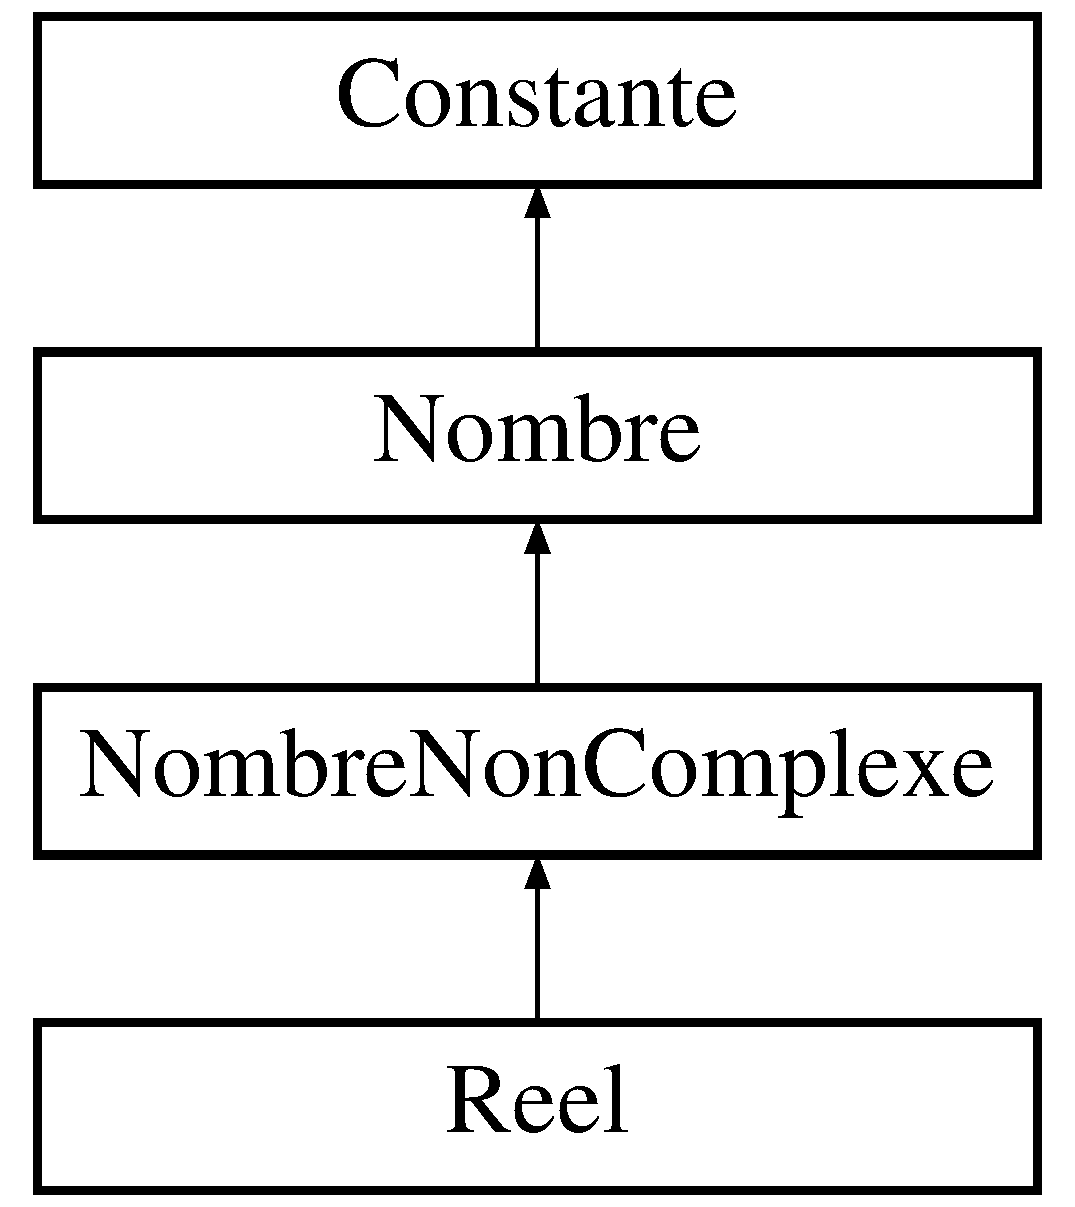
\includegraphics[height=4.000000cm]{class_reel}
\end{center}
\end{figure}
\subsection*{Public Member Functions}
\begin{DoxyCompactItemize}
\item 
\hyperlink{class_reel_a0033bef2a051ce3d8890c51ed10c27a0}{$\sim$\-Reel} ()
\begin{DoxyCompactList}\small\item\em Destructeur de la classe. \end{DoxyCompactList}\item 
\hyperlink{class_reel_a3656fa67f060d2808dc07f337030b537}{Reel} ()
\begin{DoxyCompactList}\small\item\em Constructeur par d�faut. \end{DoxyCompactList}\item 
\hyperlink{class_reel_a282d209abfa27c95802314cf7be000d6}{Reel} (float val)
\begin{DoxyCompactList}\small\item\em Constructeur avec param�tre. \end{DoxyCompactList}\item 
\hyperlink{class_reel_ac2134d63a195829000fa0aa500fbd7f0}{Reel} (const \hyperlink{class_reel}{Reel} \&r)
\begin{DoxyCompactList}\small\item\em Constructeur par copie. \end{DoxyCompactList}\item 
\hyperlink{class_reel}{Reel} $\ast$ \hyperlink{class_reel_ab53c7d10a93c702bd7ccde897fc396df}{clone} () const 
\begin{DoxyCompactList}\small\item\em M�thode permettant de cloner une constante.  \end{DoxyCompactList}\item 
float \hyperlink{class_reel_a66d6f1cfe4fa7665f7f83e242a816a5a}{get\-Val} () const 
\begin{DoxyCompactList}\small\item\em Getter de la valeur du r�el. \end{DoxyCompactList}\item 
void \hyperlink{class_reel_ab86c394e2e4a6729ecafba23e65915ad}{sign} ()
\begin{DoxyCompactList}\small\item\em Methode permettant de transformer le nombre en son oppos�.  \end{DoxyCompactList}\item 
void \hyperlink{class_reel_a612dd1edfce0d6fa687ab4cbfc700d07}{sqr} ()
\begin{DoxyCompactList}\small\item\em M�thode permettant de transformer le nombre en son carr�.  \end{DoxyCompactList}\item 
void \hyperlink{class_reel_ac46be5621787809b3fea257b54fee83f}{cube} ()
\begin{DoxyCompactList}\small\item\em M�thode permettant de transformer le nombre en son cube.  \end{DoxyCompactList}\item 
void \hyperlink{class_reel_a11fda3f1bd3cdac610d3a2aeec2fc7ed}{pow} (\hyperlink{class_entier}{Entier} $\ast$)
\begin{DoxyCompactList}\small\item\em M�thode permettant d'effectuer la puissance d'un nombre.  \end{DoxyCompactList}\item 
Q\-String \hyperlink{class_reel_a990e8324822ba3dbc64fc7ff727411e2}{to\-String} () const 
\begin{DoxyCompactList}\small\item\em Fonction permettant de renvoyer une chaine comprenant la valuation de la constante associ�, cette fonction est utilis�e dans le cadre de l'affichage des constantes dans la pile.  \end{DoxyCompactList}\item 
\hyperlink{class_nombre_complexe}{Nombre\-Complexe} $\ast$ \hyperlink{class_reel_a3ba5e47699a1ccff32075a588afda91e}{to\-Nombre\-Complexe} ()
\begin{DoxyCompactList}\small\item\em M�thode permettant de convertir un \hyperlink{class_nombre}{Nombre} en son �quivalent en \hyperlink{class_nombre_complexe}{Nombre\-Complexe}.  \end{DoxyCompactList}\item 
float \hyperlink{class_reel_a9d2e05f1f59ad433c3eafb2da7e09f86}{get\-Float\-Val} () const 
\begin{DoxyCompactList}\small\item\em M�thode permettant de r�cup�rer la valeur du \hyperlink{class_nombre_non_complexe}{Nombre\-Non\-Complexe} sous la forme d'un r�el.  \end{DoxyCompactList}\end{DoxyCompactItemize}


\subsection{Detailed Description}
Classe impl�mentant l'interface de \hyperlink{class_nombre_non_complexe}{Nombre\-Non\-Complexe} et permettant de g�rer les constantes de type reel. 

Definition at line 21 of file reel.\-h.



\subsection{Constructor \& Destructor Documentation}
\hypertarget{class_reel_a0033bef2a051ce3d8890c51ed10c27a0}{\index{Reel@{Reel}!$\sim$\-Reel@{$\sim$\-Reel}}
\index{$\sim$\-Reel@{$\sim$\-Reel}!Reel@{Reel}}
\subsubsection[{$\sim$\-Reel}]{\setlength{\rightskip}{0pt plus 5cm}{\bf Reel\-::$\sim$\-Reel} (
\begin{DoxyParamCaption}
{}
\end{DoxyParamCaption}
)\hspace{0.3cm}{\ttfamily  \mbox{[}inline\mbox{]}}}}\label{class_reel_a0033bef2a051ce3d8890c51ed10c27a0}


Destructeur de la classe. 



Definition at line 31 of file reel.\-h.

\hypertarget{class_reel_a3656fa67f060d2808dc07f337030b537}{\index{Reel@{Reel}!Reel@{Reel}}
\index{Reel@{Reel}!Reel@{Reel}}
\subsubsection[{Reel}]{\setlength{\rightskip}{0pt plus 5cm}{\bf Reel\-::\-Reel} (
\begin{DoxyParamCaption}
{}
\end{DoxyParamCaption}
)\hspace{0.3cm}{\ttfamily  \mbox{[}inline\mbox{]}}}}\label{class_reel_a3656fa67f060d2808dc07f337030b537}


Constructeur par d�faut. 



Definition at line 35 of file reel.\-h.

\hypertarget{class_reel_a282d209abfa27c95802314cf7be000d6}{\index{Reel@{Reel}!Reel@{Reel}}
\index{Reel@{Reel}!Reel@{Reel}}
\subsubsection[{Reel}]{\setlength{\rightskip}{0pt plus 5cm}{\bf Reel\-::\-Reel} (
\begin{DoxyParamCaption}
\item[{float}]{val}
\end{DoxyParamCaption}
)\hspace{0.3cm}{\ttfamily  \mbox{[}inline\mbox{]}}}}\label{class_reel_a282d209abfa27c95802314cf7be000d6}


Constructeur avec param�tre. 


\begin{DoxyParams}{Parameters}
{\em val} & La valeur du r�el \\
\hline
\end{DoxyParams}


Definition at line 40 of file reel.\-h.

\hypertarget{class_reel_ac2134d63a195829000fa0aa500fbd7f0}{\index{Reel@{Reel}!Reel@{Reel}}
\index{Reel@{Reel}!Reel@{Reel}}
\subsubsection[{Reel}]{\setlength{\rightskip}{0pt plus 5cm}{\bf Reel\-::\-Reel} (
\begin{DoxyParamCaption}
\item[{const {\bf Reel} \&}]{r}
\end{DoxyParamCaption}
)\hspace{0.3cm}{\ttfamily  \mbox{[}inline\mbox{]}}}}\label{class_reel_ac2134d63a195829000fa0aa500fbd7f0}


Constructeur par copie. 


\begin{DoxyParams}{Parameters}
{\em r} & Le r�el � copier \\
\hline
\end{DoxyParams}


Definition at line 45 of file reel.\-h.



\subsection{Member Function Documentation}
\hypertarget{class_reel_ab53c7d10a93c702bd7ccde897fc396df}{\index{Reel@{Reel}!clone@{clone}}
\index{clone@{clone}!Reel@{Reel}}
\subsubsection[{clone}]{\setlength{\rightskip}{0pt plus 5cm}{\bf Reel} $\ast$ {\bf Reel\-::clone} (
\begin{DoxyParamCaption}
{}
\end{DoxyParamCaption}
) const\hspace{0.3cm}{\ttfamily  \mbox{[}virtual\mbox{]}}}}\label{class_reel_ab53c7d10a93c702bd7ccde897fc396df}


M�thode permettant de cloner une constante.  


\begin{DoxyParams}{Parameters}
{\em Le} & pointeur vers la constante clon�e \\
\hline
\end{DoxyParams}
 

Implements \hyperlink{class_constante_a5769ea385161e02bd2d1bcadefc2c510}{Constante}.



Definition at line 10 of file reel.\-cpp.

\hypertarget{class_reel_ac46be5621787809b3fea257b54fee83f}{\index{Reel@{Reel}!cube@{cube}}
\index{cube@{cube}!Reel@{Reel}}
\subsubsection[{cube}]{\setlength{\rightskip}{0pt plus 5cm}void {\bf Reel\-::cube} (
\begin{DoxyParamCaption}
{}
\end{DoxyParamCaption}
)\hspace{0.3cm}{\ttfamily  \mbox{[}inline, virtual\mbox{]}}}}\label{class_reel_ac46be5621787809b3fea257b54fee83f}


M�thode permettant de transformer le nombre en son cube.  



Implements \hyperlink{class_nombre_aed65cb1449858c078e91610afb3a6447}{Nombre}.



Definition at line 66 of file reel.\-h.

\hypertarget{class_reel_a9d2e05f1f59ad433c3eafb2da7e09f86}{\index{Reel@{Reel}!get\-Float\-Val@{get\-Float\-Val}}
\index{get\-Float\-Val@{get\-Float\-Val}!Reel@{Reel}}
\subsubsection[{get\-Float\-Val}]{\setlength{\rightskip}{0pt plus 5cm}float {\bf Reel\-::get\-Float\-Val} (
\begin{DoxyParamCaption}
{}
\end{DoxyParamCaption}
) const\hspace{0.3cm}{\ttfamily  \mbox{[}inline, virtual\mbox{]}}}}\label{class_reel_a9d2e05f1f59ad433c3eafb2da7e09f86}


M�thode permettant de r�cup�rer la valeur du \hyperlink{class_nombre_non_complexe}{Nombre\-Non\-Complexe} sous la forme d'un r�el.  

\begin{DoxyReturn}{Returns}
La valeur r�elle 
\end{DoxyReturn}
 

Implements \hyperlink{class_nombre_non_complexe_ad148f1e2a4626ecf279e91d04d1aff24}{Nombre\-Non\-Complexe}.



Definition at line 82 of file reel.\-h.

\hypertarget{class_reel_a66d6f1cfe4fa7665f7f83e242a816a5a}{\index{Reel@{Reel}!get\-Val@{get\-Val}}
\index{get\-Val@{get\-Val}!Reel@{Reel}}
\subsubsection[{get\-Val}]{\setlength{\rightskip}{0pt plus 5cm}float {\bf Reel\-::get\-Val} (
\begin{DoxyParamCaption}
{}
\end{DoxyParamCaption}
) const\hspace{0.3cm}{\ttfamily  \mbox{[}inline\mbox{]}}}}\label{class_reel_a66d6f1cfe4fa7665f7f83e242a816a5a}


Getter de la valeur du r�el. 

\begin{DoxyReturn}{Returns}
La valeur du r�el 
\end{DoxyReturn}


Definition at line 54 of file reel.\-h.

\hypertarget{class_reel_a11fda3f1bd3cdac610d3a2aeec2fc7ed}{\index{Reel@{Reel}!pow@{pow}}
\index{pow@{pow}!Reel@{Reel}}
\subsubsection[{pow}]{\setlength{\rightskip}{0pt plus 5cm}void {\bf Reel\-::pow} (
\begin{DoxyParamCaption}
\item[{{\bf Entier} $\ast$}]{e}
\end{DoxyParamCaption}
)\hspace{0.3cm}{\ttfamily  \mbox{[}virtual\mbox{]}}}}\label{class_reel_a11fda3f1bd3cdac610d3a2aeec2fc7ed}


M�thode permettant d'effectuer la puissance d'un nombre.  


\begin{DoxyParams}{Parameters}
{\em e} & Un entier correspondant � la puissance \\
\hline
\end{DoxyParams}
 

Implements \hyperlink{class_nombre_non_complexe_a859175bae737e01e73316632f1083d07}{Nombre\-Non\-Complexe}.



Definition at line 14 of file reel.\-cpp.

\hypertarget{class_reel_ab86c394e2e4a6729ecafba23e65915ad}{\index{Reel@{Reel}!sign@{sign}}
\index{sign@{sign}!Reel@{Reel}}
\subsubsection[{sign}]{\setlength{\rightskip}{0pt plus 5cm}void {\bf Reel\-::sign} (
\begin{DoxyParamCaption}
{}
\end{DoxyParamCaption}
)\hspace{0.3cm}{\ttfamily  \mbox{[}inline, virtual\mbox{]}}}}\label{class_reel_ab86c394e2e4a6729ecafba23e65915ad}


Methode permettant de transformer le nombre en son oppos�.  



Implements \hyperlink{class_nombre_a718d616bbf2e5e8f133df958e8bb3d7f}{Nombre}.



Definition at line 58 of file reel.\-h.

\hypertarget{class_reel_a612dd1edfce0d6fa687ab4cbfc700d07}{\index{Reel@{Reel}!sqr@{sqr}}
\index{sqr@{sqr}!Reel@{Reel}}
\subsubsection[{sqr}]{\setlength{\rightskip}{0pt plus 5cm}void {\bf Reel\-::sqr} (
\begin{DoxyParamCaption}
{}
\end{DoxyParamCaption}
)\hspace{0.3cm}{\ttfamily  \mbox{[}inline, virtual\mbox{]}}}}\label{class_reel_a612dd1edfce0d6fa687ab4cbfc700d07}


M�thode permettant de transformer le nombre en son carr�.  



Implements \hyperlink{class_nombre_a5be0e66e9bbec508d236ba8dbe1eb6bc}{Nombre}.



Definition at line 62 of file reel.\-h.

\hypertarget{class_reel_a3ba5e47699a1ccff32075a588afda91e}{\index{Reel@{Reel}!to\-Nombre\-Complexe@{to\-Nombre\-Complexe}}
\index{to\-Nombre\-Complexe@{to\-Nombre\-Complexe}!Reel@{Reel}}
\subsubsection[{to\-Nombre\-Complexe}]{\setlength{\rightskip}{0pt plus 5cm}{\bf Nombre\-Complexe} $\ast$ {\bf Reel\-::to\-Nombre\-Complexe} (
\begin{DoxyParamCaption}
{}
\end{DoxyParamCaption}
)\hspace{0.3cm}{\ttfamily  \mbox{[}virtual\mbox{]}}}}\label{class_reel_a3ba5e47699a1ccff32075a588afda91e}


M�thode permettant de convertir un \hyperlink{class_nombre}{Nombre} en son �quivalent en \hyperlink{class_nombre_complexe}{Nombre\-Complexe}.  

\begin{DoxyReturn}{Returns}
Le pointeur vers le nombre\-Complexe nouvellement cr�e 
\end{DoxyReturn}
 

Implements \hyperlink{class_nombre_a11092e1fcde81c05b4c518398baf3691}{Nombre}.



Definition at line 6 of file reel.\-cpp.

\hypertarget{class_reel_a990e8324822ba3dbc64fc7ff727411e2}{\index{Reel@{Reel}!to\-String@{to\-String}}
\index{to\-String@{to\-String}!Reel@{Reel}}
\subsubsection[{to\-String}]{\setlength{\rightskip}{0pt plus 5cm}Q\-String {\bf Reel\-::to\-String} (
\begin{DoxyParamCaption}
{}
\end{DoxyParamCaption}
) const\hspace{0.3cm}{\ttfamily  \mbox{[}inline, virtual\mbox{]}}}}\label{class_reel_a990e8324822ba3dbc64fc7ff727411e2}


Fonction permettant de renvoyer une chaine comprenant la valuation de la constante associ�, cette fonction est utilis�e dans le cadre de l'affichage des constantes dans la pile.  

\begin{DoxyReturn}{Returns}
La chaine � afficher dans la pile 
\end{DoxyReturn}
 

Implements \hyperlink{class_constante_ad5ea6850196ee9f86b74c74009a87ab1}{Constante}.



Definition at line 74 of file reel.\-h.



The documentation for this class was generated from the following files\-:\begin{DoxyCompactItemize}
\item 
\hyperlink{reel_8h}{reel.\-h}\item 
\hyperlink{reel_8cpp}{reel.\-cpp}\end{DoxyCompactItemize}

\hypertarget{class_settings}{\section{Settings Class Reference}
\label{class_settings}\index{Settings@{Settings}}
}


Classe (utilisant le Design Pattern Singleton) permettant de gerer les param�tres de la calculatrice (utilisee dans le cadre de la sauvegarde de contexte notamment).  




{\ttfamily \#include $<$settings.\-h$>$}

\subsection*{Public Types}
\begin{DoxyCompactItemize}
\item 
enum \hyperlink{class_settings_adb4ecdba67a8afd48e814d158660a1b3}{Utilisation\-De\-Complexe} \{ \hyperlink{class_settings_adb4ecdba67a8afd48e814d158660a1b3ab3f9ae5d2d8d1dbba5157cebb6eba9b1}{C\-O\-M\-P\-L\-E\-X\-E}, 
\hyperlink{class_settings_adb4ecdba67a8afd48e814d158660a1b3a13cf89257e83656f5747caea9cbd5b4a}{N\-O\-N\-\_\-\-C\-O\-M\-P\-L\-E\-X\-E}
 \}
\begin{DoxyCompactList}\small\item\em Le reglage concernant l'utilisation de complexe. \end{DoxyCompactList}\item 
enum \hyperlink{class_settings_a7c410b290dcc4eb1374afde392f60bfc}{Angles} \{ \hyperlink{class_settings_a7c410b290dcc4eb1374afde392f60bfca1b0c8eaf991d4d335a3832f2a9796a35}{D\-E\-G\-R\-E\-S}, 
\hyperlink{class_settings_a7c410b290dcc4eb1374afde392f60bfca55630b14579bcbf00b72a0569e5e2709}{R\-A\-D\-I\-A\-N\-S}
 \}
\begin{DoxyCompactList}\small\item\em Le reglage concernant l'unite des angles. \end{DoxyCompactList}\item 
enum \hyperlink{class_settings_a2d04760870d51e7ca8692b99914feee5}{Type\-Constante} \{ \hyperlink{class_settings_a2d04760870d51e7ca8692b99914feee5af0e47cd4d31f34f37f884a4f0fede3b1}{E\-N\-T\-I\-E\-R}, 
\hyperlink{class_settings_a2d04760870d51e7ca8692b99914feee5a459bca6cedd517b3bb4a14ac9f9b5275}{R\-A\-T\-I\-O\-N\-N\-E\-L}, 
\hyperlink{class_settings_a2d04760870d51e7ca8692b99914feee5a505d204db40572a1d7463805246fca41}{R\-E\-E\-L}
 \}
\begin{DoxyCompactList}\small\item\em Le reglage concernant le type de constante en cours d'utilisation. \end{DoxyCompactList}\end{DoxyCompactItemize}
\subsection*{Public Member Functions}
\begin{DoxyCompactItemize}
\item 
\hyperlink{class_settings_adb4ecdba67a8afd48e814d158660a1b3}{Utilisation\-De\-Complexe} \hyperlink{class_settings_a226a2f433d78c004337fe92d4f2c0de0}{get\-Utilisation\-De\-Complexe} ()
\begin{DoxyCompactList}\small\item\em getter du reglage concernant l'utilisation des complexes. \end{DoxyCompactList}\item 
void \hyperlink{class_settings_a87838a3f7856c6727777eedfdc66d978}{set\-Utilisation\-De\-Complexe} (\hyperlink{class_settings_adb4ecdba67a8afd48e814d158660a1b3}{Utilisation\-De\-Complexe} comp)
\begin{DoxyCompactList}\small\item\em setter du reglage concernant l'utilisation des complexes. \end{DoxyCompactList}\item 
\hyperlink{class_settings_a7c410b290dcc4eb1374afde392f60bfc}{Angles} \hyperlink{class_settings_a22ffe21e72ea4de6b72a277d6f40823e}{get\-Angles} ()
\begin{DoxyCompactList}\small\item\em getter du reglage concernant l'unite des angles. \end{DoxyCompactList}\item 
void \hyperlink{class_settings_a16c9352aff0f6cda8d32162f5683662f}{set\-Angles} (\hyperlink{class_settings_a7c410b290dcc4eb1374afde392f60bfc}{Angles} an)
\begin{DoxyCompactList}\small\item\em setter du reglage concernant l'unite des angles. \end{DoxyCompactList}\item 
\hyperlink{class_settings_a2d04760870d51e7ca8692b99914feee5}{Type\-Constante} \hyperlink{class_settings_aad1ece7ef8379ee45532e9fbadef4a07}{get\-Type\-Constante} ()
\begin{DoxyCompactList}\small\item\em getter du reglage concernant le type des constantes. \end{DoxyCompactList}\item 
void \hyperlink{class_settings_a04de3fa2f43190fc5cac3caa7b9070c5}{set\-Type\-Constante} (\hyperlink{class_settings_a2d04760870d51e7ca8692b99914feee5}{Type\-Constante} co)
\begin{DoxyCompactList}\small\item\em setter du reglage concernant le type des constantes. \end{DoxyCompactList}\item 
int \hyperlink{class_settings_a86d89a7e5f502b0ec628c23d0a65e15e}{get\-Nb\-Elem\-Affichable} ()
\begin{DoxyCompactList}\small\item\em getter du reglage concernant le nombre d'elements de la pile affichable. \end{DoxyCompactList}\item 
void \hyperlink{class_settings_aa1fa14a8735fb1d5c48de999d92be929}{set\-Nb\-Element\-Affichable} (int nb\-Element)
\begin{DoxyCompactList}\small\item\em setter du reglage concernant le nombre d'�l�ments � afficher dans la pile. \end{DoxyCompactList}\end{DoxyCompactItemize}
\subsection*{Static Public Member Functions}
\begin{DoxyCompactItemize}
\item 
static \hyperlink{class_settings}{Settings} $\ast$ \hyperlink{class_settings_a5134bac1c68824ef48651c8469cf8722}{get\-Instance} ()
\begin{DoxyCompactList}\small\item\em M�thode permettant de retourner l'instance de la classe \hyperlink{class_settings}{Settings}. \end{DoxyCompactList}\item 
static void \hyperlink{class_settings_a9008b343feeb2a29215dc21c22d508e0}{free\-Instance} ()
\begin{DoxyCompactList}\small\item\em M�thode permettant de lib�rer l'instance. \end{DoxyCompactList}\end{DoxyCompactItemize}


\subsection{Detailed Description}
Classe (utilisant le Design Pattern Singleton) permettant de gerer les param�tres de la calculatrice (utilisee dans le cadre de la sauvegarde de contexte notamment). 

Definition at line 17 of file settings.\-h.



\subsection{Member Enumeration Documentation}
\hypertarget{class_settings_a7c410b290dcc4eb1374afde392f60bfc}{\index{Settings@{Settings}!Angles@{Angles}}
\index{Angles@{Angles}!Settings@{Settings}}
\subsubsection[{Angles}]{\setlength{\rightskip}{0pt plus 5cm}enum {\bf Settings\-::\-Angles}}}\label{class_settings_a7c410b290dcc4eb1374afde392f60bfc}


Le reglage concernant l'unite des angles. 

\begin{Desc}
\item[Enumerator\-: ]\par
\begin{description}
\index{D\-E\-G\-R\-E\-S@{D\-E\-G\-R\-E\-S}!Settings@{Settings}}\index{Settings@{Settings}!D\-E\-G\-R\-E\-S@{D\-E\-G\-R\-E\-S}}\item[{\em 
\hypertarget{class_settings_a7c410b290dcc4eb1374afde392f60bfca1b0c8eaf991d4d335a3832f2a9796a35}{D\-E\-G\-R\-E\-S}\label{class_settings_a7c410b290dcc4eb1374afde392f60bfca1b0c8eaf991d4d335a3832f2a9796a35}
}]Les angles sont exprimes en degres. \index{R\-A\-D\-I\-A\-N\-S@{R\-A\-D\-I\-A\-N\-S}!Settings@{Settings}}\index{Settings@{Settings}!R\-A\-D\-I\-A\-N\-S@{R\-A\-D\-I\-A\-N\-S}}\item[{\em 
\hypertarget{class_settings_a7c410b290dcc4eb1374afde392f60bfca55630b14579bcbf00b72a0569e5e2709}{R\-A\-D\-I\-A\-N\-S}\label{class_settings_a7c410b290dcc4eb1374afde392f60bfca55630b14579bcbf00b72a0569e5e2709}
}]Les angles sont exprimees en radians. \end{description}
\end{Desc}



Definition at line 33 of file settings.\-h.

\hypertarget{class_settings_a2d04760870d51e7ca8692b99914feee5}{\index{Settings@{Settings}!Type\-Constante@{Type\-Constante}}
\index{Type\-Constante@{Type\-Constante}!Settings@{Settings}}
\subsubsection[{Type\-Constante}]{\setlength{\rightskip}{0pt plus 5cm}enum {\bf Settings\-::\-Type\-Constante}}}\label{class_settings_a2d04760870d51e7ca8692b99914feee5}


Le reglage concernant le type de constante en cours d'utilisation. 

\begin{Desc}
\item[Enumerator\-: ]\par
\begin{description}
\index{E\-N\-T\-I\-E\-R@{E\-N\-T\-I\-E\-R}!Settings@{Settings}}\index{Settings@{Settings}!E\-N\-T\-I\-E\-R@{E\-N\-T\-I\-E\-R}}\item[{\em 
\hypertarget{class_settings_a2d04760870d51e7ca8692b99914feee5af0e47cd4d31f34f37f884a4f0fede3b1}{E\-N\-T\-I\-E\-R}\label{class_settings_a2d04760870d51e7ca8692b99914feee5af0e47cd4d31f34f37f884a4f0fede3b1}
}]Les constantes utilisees sont de type entier. \index{R\-A\-T\-I\-O\-N\-N\-E\-L@{R\-A\-T\-I\-O\-N\-N\-E\-L}!Settings@{Settings}}\index{Settings@{Settings}!R\-A\-T\-I\-O\-N\-N\-E\-L@{R\-A\-T\-I\-O\-N\-N\-E\-L}}\item[{\em 
\hypertarget{class_settings_a2d04760870d51e7ca8692b99914feee5a459bca6cedd517b3bb4a14ac9f9b5275}{R\-A\-T\-I\-O\-N\-N\-E\-L}\label{class_settings_a2d04760870d51e7ca8692b99914feee5a459bca6cedd517b3bb4a14ac9f9b5275}
}]Les constantes utilisees sont de type rationnel. \index{R\-E\-E\-L@{R\-E\-E\-L}!Settings@{Settings}}\index{Settings@{Settings}!R\-E\-E\-L@{R\-E\-E\-L}}\item[{\em 
\hypertarget{class_settings_a2d04760870d51e7ca8692b99914feee5a505d204db40572a1d7463805246fca41}{R\-E\-E\-L}\label{class_settings_a2d04760870d51e7ca8692b99914feee5a505d204db40572a1d7463805246fca41}
}]Les constantes utilisees sont de type reel. \end{description}
\end{Desc}



Definition at line 43 of file settings.\-h.

\hypertarget{class_settings_adb4ecdba67a8afd48e814d158660a1b3}{\index{Settings@{Settings}!Utilisation\-De\-Complexe@{Utilisation\-De\-Complexe}}
\index{Utilisation\-De\-Complexe@{Utilisation\-De\-Complexe}!Settings@{Settings}}
\subsubsection[{Utilisation\-De\-Complexe}]{\setlength{\rightskip}{0pt plus 5cm}enum {\bf Settings\-::\-Utilisation\-De\-Complexe}}}\label{class_settings_adb4ecdba67a8afd48e814d158660a1b3}


Le reglage concernant l'utilisation de complexe. 

\begin{Desc}
\item[Enumerator\-: ]\par
\begin{description}
\index{C\-O\-M\-P\-L\-E\-X\-E@{C\-O\-M\-P\-L\-E\-X\-E}!Settings@{Settings}}\index{Settings@{Settings}!C\-O\-M\-P\-L\-E\-X\-E@{C\-O\-M\-P\-L\-E\-X\-E}}\item[{\em 
\hypertarget{class_settings_adb4ecdba67a8afd48e814d158660a1b3ab3f9ae5d2d8d1dbba5157cebb6eba9b1}{C\-O\-M\-P\-L\-E\-X\-E}\label{class_settings_adb4ecdba67a8afd48e814d158660a1b3ab3f9ae5d2d8d1dbba5157cebb6eba9b1}
}]L'utilisation des complexes est autorisee. \index{N\-O\-N\-\_\-\-C\-O\-M\-P\-L\-E\-X\-E@{N\-O\-N\-\_\-\-C\-O\-M\-P\-L\-E\-X\-E}!Settings@{Settings}}\index{Settings@{Settings}!N\-O\-N\-\_\-\-C\-O\-M\-P\-L\-E\-X\-E@{N\-O\-N\-\_\-\-C\-O\-M\-P\-L\-E\-X\-E}}\item[{\em 
\hypertarget{class_settings_adb4ecdba67a8afd48e814d158660a1b3a13cf89257e83656f5747caea9cbd5b4a}{N\-O\-N\-\_\-\-C\-O\-M\-P\-L\-E\-X\-E}\label{class_settings_adb4ecdba67a8afd48e814d158660a1b3a13cf89257e83656f5747caea9cbd5b4a}
}]L'utilisation des complexes n'est pas autorisee. \end{description}
\end{Desc}



Definition at line 23 of file settings.\-h.



\subsection{Member Function Documentation}
\hypertarget{class_settings_a9008b343feeb2a29215dc21c22d508e0}{\index{Settings@{Settings}!free\-Instance@{free\-Instance}}
\index{free\-Instance@{free\-Instance}!Settings@{Settings}}
\subsubsection[{free\-Instance}]{\setlength{\rightskip}{0pt plus 5cm}void {\bf Settings\-::free\-Instance} (
\begin{DoxyParamCaption}
{}
\end{DoxyParamCaption}
)\hspace{0.3cm}{\ttfamily  \mbox{[}static\mbox{]}}}}\label{class_settings_a9008b343feeb2a29215dc21c22d508e0}


M�thode permettant de lib�rer l'instance. 



Definition at line 26 of file settings.\-cpp.

\hypertarget{class_settings_a22ffe21e72ea4de6b72a277d6f40823e}{\index{Settings@{Settings}!get\-Angles@{get\-Angles}}
\index{get\-Angles@{get\-Angles}!Settings@{Settings}}
\subsubsection[{get\-Angles}]{\setlength{\rightskip}{0pt plus 5cm}{\bf Angles} {\bf Settings\-::get\-Angles} (
\begin{DoxyParamCaption}
{}
\end{DoxyParamCaption}
)\hspace{0.3cm}{\ttfamily  \mbox{[}inline\mbox{]}}}}\label{class_settings_a22ffe21e72ea4de6b72a277d6f40823e}


getter du reglage concernant l'unite des angles. 

\begin{DoxyReturn}{Returns}
L'unit� d'angles utilis�e 
\end{DoxyReturn}


Definition at line 112 of file settings.\-h.

\hypertarget{class_settings_a5134bac1c68824ef48651c8469cf8722}{\index{Settings@{Settings}!get\-Instance@{get\-Instance}}
\index{get\-Instance@{get\-Instance}!Settings@{Settings}}
\subsubsection[{get\-Instance}]{\setlength{\rightskip}{0pt plus 5cm}{\bf Settings} $\ast$ {\bf Settings\-::get\-Instance} (
\begin{DoxyParamCaption}
{}
\end{DoxyParamCaption}
)\hspace{0.3cm}{\ttfamily  \mbox{[}static\mbox{]}}}}\label{class_settings_a5134bac1c68824ef48651c8469cf8722}


M�thode permettant de retourner l'instance de la classe \hyperlink{class_settings}{Settings}. 

\begin{DoxyReturn}{Returns}
L'instance 
\end{DoxyReturn}


Definition at line 20 of file settings.\-cpp.

\hypertarget{class_settings_a86d89a7e5f502b0ec628c23d0a65e15e}{\index{Settings@{Settings}!get\-Nb\-Elem\-Affichable@{get\-Nb\-Elem\-Affichable}}
\index{get\-Nb\-Elem\-Affichable@{get\-Nb\-Elem\-Affichable}!Settings@{Settings}}
\subsubsection[{get\-Nb\-Elem\-Affichable}]{\setlength{\rightskip}{0pt plus 5cm}int {\bf Settings\-::get\-Nb\-Elem\-Affichable} (
\begin{DoxyParamCaption}
{}
\end{DoxyParamCaption}
)\hspace{0.3cm}{\ttfamily  \mbox{[}inline\mbox{]}}}}\label{class_settings_a86d89a7e5f502b0ec628c23d0a65e15e}


getter du reglage concernant le nombre d'elements de la pile affichable. 

\begin{DoxyReturn}{Returns}
Le nombre d'�l�ments de la pile � afficher 
\end{DoxyReturn}


Definition at line 140 of file settings.\-h.

\hypertarget{class_settings_aad1ece7ef8379ee45532e9fbadef4a07}{\index{Settings@{Settings}!get\-Type\-Constante@{get\-Type\-Constante}}
\index{get\-Type\-Constante@{get\-Type\-Constante}!Settings@{Settings}}
\subsubsection[{get\-Type\-Constante}]{\setlength{\rightskip}{0pt plus 5cm}{\bf Type\-Constante} {\bf Settings\-::get\-Type\-Constante} (
\begin{DoxyParamCaption}
{}
\end{DoxyParamCaption}
)\hspace{0.3cm}{\ttfamily  \mbox{[}inline\mbox{]}}}}\label{class_settings_aad1ece7ef8379ee45532e9fbadef4a07}


getter du reglage concernant le type des constantes. 

\begin{DoxyReturn}{Returns}
Le type de constante utilis� 
\end{DoxyReturn}


Definition at line 126 of file settings.\-h.

\hypertarget{class_settings_a226a2f433d78c004337fe92d4f2c0de0}{\index{Settings@{Settings}!get\-Utilisation\-De\-Complexe@{get\-Utilisation\-De\-Complexe}}
\index{get\-Utilisation\-De\-Complexe@{get\-Utilisation\-De\-Complexe}!Settings@{Settings}}
\subsubsection[{get\-Utilisation\-De\-Complexe}]{\setlength{\rightskip}{0pt plus 5cm}{\bf Utilisation\-De\-Complexe} {\bf Settings\-::get\-Utilisation\-De\-Complexe} (
\begin{DoxyParamCaption}
{}
\end{DoxyParamCaption}
)\hspace{0.3cm}{\ttfamily  \mbox{[}inline\mbox{]}}}}\label{class_settings_a226a2f433d78c004337fe92d4f2c0de0}


getter du reglage concernant l'utilisation des complexes. 

\begin{DoxyReturn}{Returns}
L'utilisation ou non des complexes 
\end{DoxyReturn}


Definition at line 98 of file settings.\-h.

\hypertarget{class_settings_a16c9352aff0f6cda8d32162f5683662f}{\index{Settings@{Settings}!set\-Angles@{set\-Angles}}
\index{set\-Angles@{set\-Angles}!Settings@{Settings}}
\subsubsection[{set\-Angles}]{\setlength{\rightskip}{0pt plus 5cm}void {\bf Settings\-::set\-Angles} (
\begin{DoxyParamCaption}
\item[{{\bf Angles}}]{an}
\end{DoxyParamCaption}
)\hspace{0.3cm}{\ttfamily  \mbox{[}inline\mbox{]}}}}\label{class_settings_a16c9352aff0f6cda8d32162f5683662f}


setter du reglage concernant l'unite des angles. 


\begin{DoxyParams}{Parameters}
{\em an} & Angles \\
\hline
\end{DoxyParams}


Definition at line 119 of file settings.\-h.

\hypertarget{class_settings_aa1fa14a8735fb1d5c48de999d92be929}{\index{Settings@{Settings}!set\-Nb\-Element\-Affichable@{set\-Nb\-Element\-Affichable}}
\index{set\-Nb\-Element\-Affichable@{set\-Nb\-Element\-Affichable}!Settings@{Settings}}
\subsubsection[{set\-Nb\-Element\-Affichable}]{\setlength{\rightskip}{0pt plus 5cm}void {\bf Settings\-::set\-Nb\-Element\-Affichable} (
\begin{DoxyParamCaption}
\item[{int}]{nb\-Element}
\end{DoxyParamCaption}
)}}\label{class_settings_aa1fa14a8735fb1d5c48de999d92be929}


setter du reglage concernant le nombre d'�l�ments � afficher dans la pile. 


\begin{DoxyParams}{Parameters}
{\em nb\-Element} & \hyperlink{class_nombre}{Nombre} d'�l�ments de la pile � afficher \\
\hline
\end{DoxyParams}


Definition at line 31 of file settings.\-cpp.

\hypertarget{class_settings_a04de3fa2f43190fc5cac3caa7b9070c5}{\index{Settings@{Settings}!set\-Type\-Constante@{set\-Type\-Constante}}
\index{set\-Type\-Constante@{set\-Type\-Constante}!Settings@{Settings}}
\subsubsection[{set\-Type\-Constante}]{\setlength{\rightskip}{0pt plus 5cm}void {\bf Settings\-::set\-Type\-Constante} (
\begin{DoxyParamCaption}
\item[{{\bf Type\-Constante}}]{co}
\end{DoxyParamCaption}
)\hspace{0.3cm}{\ttfamily  \mbox{[}inline\mbox{]}}}}\label{class_settings_a04de3fa2f43190fc5cac3caa7b9070c5}


setter du reglage concernant le type des constantes. 


\begin{DoxyParams}{Parameters}
{\em co} & Type\-Constante \\
\hline
\end{DoxyParams}


Definition at line 133 of file settings.\-h.

\hypertarget{class_settings_a87838a3f7856c6727777eedfdc66d978}{\index{Settings@{Settings}!set\-Utilisation\-De\-Complexe@{set\-Utilisation\-De\-Complexe}}
\index{set\-Utilisation\-De\-Complexe@{set\-Utilisation\-De\-Complexe}!Settings@{Settings}}
\subsubsection[{set\-Utilisation\-De\-Complexe}]{\setlength{\rightskip}{0pt plus 5cm}void {\bf Settings\-::set\-Utilisation\-De\-Complexe} (
\begin{DoxyParamCaption}
\item[{{\bf Utilisation\-De\-Complexe}}]{comp}
\end{DoxyParamCaption}
)\hspace{0.3cm}{\ttfamily  \mbox{[}inline\mbox{]}}}}\label{class_settings_a87838a3f7856c6727777eedfdc66d978}


setter du reglage concernant l'utilisation des complexes. 


\begin{DoxyParams}{Parameters}
{\em comp} & Utilisation\-De\-Complexe \\
\hline
\end{DoxyParams}


Definition at line 105 of file settings.\-h.



The documentation for this class was generated from the following files\-:\begin{DoxyCompactItemize}
\item 
\hyperlink{settings_8h}{settings.\-h}\item 
\hyperlink{settings_8cpp}{settings.\-cpp}\end{DoxyCompactItemize}

\chapter{File Documentation}
\hypertarget{constante_8cpp}{\section{constante.\-cpp File Reference}
\label{constante_8cpp}\index{constante.\-cpp@{constante.\-cpp}}
}

\hypertarget{constante_8h}{\section{constante.\-h File Reference}
\label{constante_8h}\index{constante.\-h@{constante.\-h}}
}
{\ttfamily \#include \char`\"{}log\-Message.\-h\char`\"{}}\\*
{\ttfamily \#include \char`\"{}settings.\-h\char`\"{}}\\*
\subsection*{Classes}
\begin{DoxyCompactItemize}
\item 
class \hyperlink{class_constante}{Constante}
\begin{DoxyCompactList}\small\item\em Interface (utilisant le design pattern composite) permettant de g�rer les diff�rents types de valeurs qui peuvent �tre empil�es sur la pile. \end{DoxyCompactList}\end{DoxyCompactItemize}


\subsection{Detailed Description}
\begin{DoxyAuthor}{Author}
Sebastien Fradcourt \& Florian Dufrot 
\end{DoxyAuthor}
\begin{DoxyDate}{Date}
24 Mai 2012 
\end{DoxyDate}
\begin{DoxyVersion}{Version}
1.\-0 
\end{DoxyVersion}


Definition in file \hyperlink{constante_8h_source}{constante.\-h}.


\hypertarget{constantefactory_8cpp}{\section{constantefactory.\-cpp File Reference}
\label{constantefactory_8cpp}\index{constantefactory.\-cpp@{constantefactory.\-cpp}}
}
{\ttfamily \#include \char`\"{}constante\-Factory.\-h\char`\"{}}\\*
{\ttfamily \#include \char`\"{}entier.\-h\char`\"{}}\\*
{\ttfamily \#include \char`\"{}expression.\-h\char`\"{}}\\*
{\ttfamily \#include \char`\"{}rationnel.\-h\char`\"{}}\\*
{\ttfamily \#include \char`\"{}reel.\-h\char`\"{}}\\*
{\ttfamily \#include \char`\"{}nombre\-Complexe.\-h\char`\"{}}\\*
{\ttfamily \#include \char`\"{}operateur.\-h\char`\"{}}\\*
{\ttfamily \#include \char`\"{}settings.\-h\char`\"{}}\\*

\hypertarget{constante_factory_8h}{\section{constante\-Factory.\-h File Reference}
\label{constante_factory_8h}\index{constante\-Factory.\-h@{constante\-Factory.\-h}}
}
{\ttfamily \#include $<$Q\-String$>$}\\*
{\ttfamily \#include $<$Q\-Reg\-Exp$>$}\\*
{\ttfamily \#include \char`\"{}constante.\-h\char`\"{}}\\*
\subsection*{Classes}
\begin{DoxyCompactItemize}
\item 
class \hyperlink{class_constante_factory}{Constante\-Factory}
\begin{DoxyCompactList}\small\item\em Classe (utilisant le Design Pattern Factory) permettant d'instancier des objets de type \hyperlink{class_constante}{Constante}. \end{DoxyCompactList}\end{DoxyCompactItemize}


\subsection{Detailed Description}
\begin{DoxyAuthor}{Author}
Sebastien Fradcourt \& Florian Dufrot 
\end{DoxyAuthor}
\begin{DoxyDate}{Date}
22 Mai 2012 
\end{DoxyDate}
\begin{DoxyVersion}{Version}
1.\-0 
\end{DoxyVersion}


Definition in file \hyperlink{constante_factory_8h_source}{constante\-Factory.\-h}.


\hypertarget{context_8cpp}{\section{context.\-cpp File Reference}
\label{context_8cpp}\index{context.\-cpp@{context.\-cpp}}
}
{\ttfamily \#include \char`\"{}context.\-h\char`\"{}}\\*
{\ttfamily \#include \char`\"{}qsettings.\-h\char`\"{}}\\*
{\ttfamily \#include \char`\"{}qdebug.\-h\char`\"{}}\\*
{\ttfamily \#include \char`\"{}Qt\-Xml/\-Q\-Dom\-Document\char`\"{}}\\*

\hypertarget{context_8h}{\section{context.\-h File Reference}
\label{context_8h}\index{context.\-h@{context.\-h}}
}
{\ttfamily \#include \char`\"{}mainwindow.\-h\char`\"{}}\\*
{\ttfamily \#include $<$iostream$>$}\\*
{\ttfamily \#include $<$fstream$>$}\\*
\subsection*{Classes}
\begin{DoxyCompactItemize}
\item 
class \hyperlink{class_context}{Context}
\begin{DoxyCompactList}\small\item\em Classe (utilisant le Design Pattern Singleton) permettant de g�rer l'�criture du context afin de pouvoir le recharger lors de l'ouverture de l'application. \end{DoxyCompactList}\end{DoxyCompactItemize}


\subsection{Detailed Description}
\begin{DoxyAuthor}{Author}
Sebastien Fradcourt \& Florian Dufrot 
\end{DoxyAuthor}
\begin{DoxyDate}{Date}
24 Mai 2012 
\end{DoxyDate}
\begin{DoxyVersion}{Version}
1.\-0 
\end{DoxyVersion}


Definition in file \hyperlink{context_8h_source}{context.\-h}.


\hypertarget{entier_8cpp}{\section{entier.\-cpp File Reference}
\label{entier_8cpp}\index{entier.\-cpp@{entier.\-cpp}}
}
{\ttfamily \#include \char`\"{}entier.\-h\char`\"{}}\\*
{\ttfamily \#include \char`\"{}reel.\-h\char`\"{}}\\*
{\ttfamily \#include \char`\"{}rationnel.\-h\char`\"{}}\\*
{\ttfamily \#include \char`\"{}nombre\-Complexe.\-h\char`\"{}}\\*

\hypertarget{entier_8h}{\section{entier.\-h File Reference}
\label{entier_8h}\index{entier.\-h@{entier.\-h}}
}
{\ttfamily \#include \char`\"{}nombre\-Non\-Complexe.\-h\char`\"{}}\\*
\subsection*{Classes}
\begin{DoxyCompactItemize}
\item 
class \hyperlink{class_entier}{Entier}
\begin{DoxyCompactList}\small\item\em Classe impl�mentant l'interface de \hyperlink{class_nombre_non_complexe}{Nombre\-Non\-Complexe} et permettant de g�rer des constantes de type entier. \end{DoxyCompactList}\end{DoxyCompactItemize}


\subsection{Detailed Description}
\begin{DoxyAuthor}{Author}
Sebastien Fradcourt \& Florian Dufrot 
\end{DoxyAuthor}
\begin{DoxyDate}{Date}
24 Mai 2012 
\end{DoxyDate}
\begin{DoxyVersion}{Version}
1.\-0 
\end{DoxyVersion}


Definition in file \hyperlink{entier_8h_source}{entier.\-h}.


\hypertarget{expression_8cpp}{\section{expression.\-cpp File Reference}
\label{expression_8cpp}\index{expression.\-cpp@{expression.\-cpp}}
}
{\ttfamily \#include \char`\"{}expression.\-h\char`\"{}}\\*
{\ttfamily \#include \char`\"{}mainwindow.\-h\char`\"{}}\\*
{\ttfamily \#include \char`\"{}operateur.\-h\char`\"{}}\\*

\hypertarget{expression_8h}{\section{expression.\-h File Reference}
\label{expression_8h}\index{expression.\-h@{expression.\-h}}
}
{\ttfamily \#include \char`\"{}constante.\-h\char`\"{}}\\*
{\ttfamily \#include \char`\"{}Q\-String.\-h\char`\"{}}\\*
{\ttfamily \#include \char`\"{}qvector.\-h\char`\"{}}\\*
{\ttfamily \#include \char`\"{}qstringlist.\-h\char`\"{}}\\*
\subsection*{Classes}
\begin{DoxyCompactItemize}
\item 
class \hyperlink{class_expression}{Expression}
\begin{DoxyCompactList}\small\item\em Classe impl�mentant l'interface de \hyperlink{class_constante}{Constante} et permettant la gestion d'un expression. \end{DoxyCompactList}\end{DoxyCompactItemize}


\subsection{Detailed Description}
\begin{DoxyAuthor}{Author}
Sebastien Fradcourt \& Florian Dufrot 
\end{DoxyAuthor}
\begin{DoxyDate}{Date}
24 Mai 2012 
\end{DoxyDate}
\begin{DoxyVersion}{Version}
1.\-0 
\end{DoxyVersion}


Definition in file \hyperlink{expression_8h_source}{expression.\-h}.


\hypertarget{historique_8cpp}{\section{historique.\-cpp File Reference}
\label{historique_8cpp}\index{historique.\-cpp@{historique.\-cpp}}
}

\hypertarget{historique_8h}{\section{historique.\-h File Reference}
\label{historique_8h}\index{historique.\-h@{historique.\-h}}
}
\subsection*{Classes}
\begin{DoxyCompactItemize}
\item 
class \hyperlink{class_historique}{Historique}
\begin{DoxyCompactList}\small\item\em Classe (utilisant le design pattern command) abstraite permettant de g�rer des objets de type \hyperlink{class_historique}{Historique}. \end{DoxyCompactList}\end{DoxyCompactItemize}


\subsection{Detailed Description}
\begin{DoxyAuthor}{Author}
Sebastien Fradcourt \& Florian Dufrot 
\end{DoxyAuthor}
\begin{DoxyDate}{Date}
03 Juin 2012 
\end{DoxyDate}
\begin{DoxyVersion}{Version}
1.\-0 
\end{DoxyVersion}


Definition in file \hyperlink{historique_8h_source}{historique.\-h}.


\hypertarget{historique_operateur_binaire_8cpp}{\section{historique\-Operateur\-Binaire.\-cpp File Reference}
\label{historique_operateur_binaire_8cpp}\index{historique\-Operateur\-Binaire.\-cpp@{historique\-Operateur\-Binaire.\-cpp}}
}
{\ttfamily \#include \char`\"{}historique\-Operateur\-Binaire.\-h\char`\"{}}\\*
{\ttfamily \#include \char`\"{}mainwindow.\-h\char`\"{}}\\*

\hypertarget{historique_operateur_binaire_8h}{\section{historique\-Operateur\-Binaire.\-h File Reference}
\label{historique_operateur_binaire_8h}\index{historique\-Operateur\-Binaire.\-h@{historique\-Operateur\-Binaire.\-h}}
}
{\ttfamily \#include \char`\"{}historique.\-h\char`\"{}}\\*
{\ttfamily \#include \char`\"{}constante.\-h\char`\"{}}\\*
\subsection*{Classes}
\begin{DoxyCompactItemize}
\item 
class \hyperlink{class_historique_operateur_binaire}{Historique\-Operateur\-Binaire}
\begin{DoxyCompactList}\small\item\em Classe impl�mentant l'interface \hyperlink{class_historique}{Historique} et permettant de g�rer l'historique de toute les commandes binaires. \end{DoxyCompactList}\end{DoxyCompactItemize}


\subsection{Detailed Description}
\begin{DoxyAuthor}{Author}
Sebastien Fradcourt \& Florian Dufrot 
\end{DoxyAuthor}
\begin{DoxyDate}{Date}
03 Juin 2012 
\end{DoxyDate}
\begin{DoxyVersion}{Version}
1.\-0 
\end{DoxyVersion}


Definition in file \hyperlink{historique_operateur_binaire_8h_source}{historique\-Operateur\-Binaire.\-h}.


\hypertarget{historique_operateur_push_8cpp}{\section{historique\-Operateur\-Push.\-cpp File Reference}
\label{historique_operateur_push_8cpp}\index{historique\-Operateur\-Push.\-cpp@{historique\-Operateur\-Push.\-cpp}}
}
{\ttfamily \#include \char`\"{}historique\-Operateur\-Push.\-h\char`\"{}}\\*
{\ttfamily \#include \char`\"{}mainwindow.\-h\char`\"{}}\\*

\hypertarget{historique_operateur_push_8h}{\section{historique\-Operateur\-Push.\-h File Reference}
\label{historique_operateur_push_8h}\index{historique\-Operateur\-Push.\-h@{historique\-Operateur\-Push.\-h}}
}
{\ttfamily \#include \char`\"{}historique.\-h\char`\"{}}\\*
{\ttfamily \#include \char`\"{}constante.\-h\char`\"{}}\\*
\subsection*{Classes}
\begin{DoxyCompactItemize}
\item 
class \hyperlink{class_historique_operateur_push}{Historique\-Operateur\-Push}
\begin{DoxyCompactList}\small\item\em Classe impl�mentant l'interface \hyperlink{class_historique}{Historique} et permettant de g�rer l'historique de tous les push. \end{DoxyCompactList}\end{DoxyCompactItemize}


\subsection{Detailed Description}
\begin{DoxyAuthor}{Author}
Sebastien Fradcourt \& Florian Dufrot 
\end{DoxyAuthor}
\begin{DoxyDate}{Date}
03 Juin 2012 
\end{DoxyDate}
\begin{DoxyVersion}{Version}
1.\-0 
\end{DoxyVersion}


Definition in file \hyperlink{historique_operateur_push_8h_source}{historique\-Operateur\-Push.\-h}.


\hypertarget{historique_operateur_sum_mean_8cpp}{\section{historique\-Operateur\-Sum\-Mean.\-cpp File Reference}
\label{historique_operateur_sum_mean_8cpp}\index{historique\-Operateur\-Sum\-Mean.\-cpp@{historique\-Operateur\-Sum\-Mean.\-cpp}}
}
{\ttfamily \#include \char`\"{}historique\-Operateur\-Sum\-Mean.\-h\char`\"{}}\\*
{\ttfamily \#include \char`\"{}mainwindow.\-h\char`\"{}}\\*

\hypertarget{historique_operateur_sum_mean_8h}{\section{historique\-Operateur\-Sum\-Mean.\-h File Reference}
\label{historique_operateur_sum_mean_8h}\index{historique\-Operateur\-Sum\-Mean.\-h@{historique\-Operateur\-Sum\-Mean.\-h}}
}
{\ttfamily \#include \char`\"{}historique.\-h\char`\"{}}\\*
{\ttfamily \#include \char`\"{}constante.\-h\char`\"{}}\\*
{\ttfamily \#include \char`\"{}qstack.\-h\char`\"{}}\\*
\subsection*{Classes}
\begin{DoxyCompactItemize}
\item 
class \hyperlink{class_historique_operateur_sum_mean}{Historique\-Operateur\-Sum\-Mean}
\begin{DoxyCompactList}\small\item\em Classe impl�mentant l'interface \hyperlink{class_historique}{Historique} et permettant de g�rer l'historique des commandes \char`\"{}sum\char`\"{} et \char`\"{}mean\char`\"{}. \end{DoxyCompactList}\end{DoxyCompactItemize}


\subsection{Detailed Description}
\begin{DoxyAuthor}{Author}
Sebastien Fradcourt \& Florian Dufrot 
\end{DoxyAuthor}
\begin{DoxyDate}{Date}
03 Juin 2012 
\end{DoxyDate}
\begin{DoxyVersion}{Version}
1.\-0 
\end{DoxyVersion}


Definition in file \hyperlink{historique_operateur_sum_mean_8h_source}{historique\-Operateur\-Sum\-Mean.\-h}.


\hypertarget{historique_operateur_swap_8cpp}{\section{historique\-Operateur\-Swap.\-cpp File Reference}
\label{historique_operateur_swap_8cpp}\index{historique\-Operateur\-Swap.\-cpp@{historique\-Operateur\-Swap.\-cpp}}
}
{\ttfamily \#include \char`\"{}historique\-Operateur\-Swap.\-h\char`\"{}}\\*
{\ttfamily \#include \char`\"{}mainwindow.\-h\char`\"{}}\\*

\hypertarget{historique_operateur_swap_8h}{\section{historique\-Operateur\-Swap.\-h File Reference}
\label{historique_operateur_swap_8h}\index{historique\-Operateur\-Swap.\-h@{historique\-Operateur\-Swap.\-h}}
}
{\ttfamily \#include \char`\"{}historique.\-h\char`\"{}}\\*
{\ttfamily \#include \char`\"{}entier.\-h\char`\"{}}\\*
\subsection*{Classes}
\begin{DoxyCompactItemize}
\item 
class \hyperlink{class_historique_operateur_swap}{Historique\-Operateur\-Swap}
\begin{DoxyCompactList}\small\item\em Classe impl�mentant l'interface \hyperlink{class_historique}{Historique} et permettant de g�rer l'historique de la commande swap. \end{DoxyCompactList}\end{DoxyCompactItemize}


\subsection{Detailed Description}
\begin{DoxyAuthor}{Author}
Sebastien Fradcourt \& Florian Dufrot 
\end{DoxyAuthor}
\begin{DoxyDate}{Date}
03 Juin 2012 
\end{DoxyDate}
\begin{DoxyVersion}{Version}
1.\-0 
\end{DoxyVersion}


Definition in file \hyperlink{historique_operateur_swap_8h_source}{historique\-Operateur\-Swap.\-h}.


\hypertarget{historique_operateur_unaire_8cpp}{\section{historique\-Operateur\-Unaire.\-cpp File Reference}
\label{historique_operateur_unaire_8cpp}\index{historique\-Operateur\-Unaire.\-cpp@{historique\-Operateur\-Unaire.\-cpp}}
}
{\ttfamily \#include \char`\"{}historique\-Operateur\-Unaire.\-h\char`\"{}}\\*
{\ttfamily \#include \char`\"{}mainwindow.\-h\char`\"{}}\\*

\hypertarget{historique_operateur_unaire_8h}{\section{historique\-Operateur\-Unaire.\-h File Reference}
\label{historique_operateur_unaire_8h}\index{historique\-Operateur\-Unaire.\-h@{historique\-Operateur\-Unaire.\-h}}
}
{\ttfamily \#include \char`\"{}historique.\-h\char`\"{}}\\*
{\ttfamily \#include \char`\"{}constante.\-h\char`\"{}}\\*
\subsection*{Classes}
\begin{DoxyCompactItemize}
\item 
class \hyperlink{class_historique_operateur_unaire}{Historique\-Operateur\-Unaire}
\begin{DoxyCompactList}\small\item\em Classe impl�mentant l'interface \hyperlink{class_historique}{Historique} et permettant de g�rer l'historique des commandes unaires. \end{DoxyCompactList}\end{DoxyCompactItemize}


\subsection{Detailed Description}
\begin{DoxyAuthor}{Author}
Sebastien Fradcourt \& Florian Dufrot 
\end{DoxyAuthor}
\begin{DoxyDate}{Date}
03 Juin 2012 
\end{DoxyDate}
\begin{DoxyVersion}{Version}
1.\-0 
\end{DoxyVersion}


Definition in file \hyperlink{historique_operateur_unaire_8h_source}{historique\-Operateur\-Unaire.\-h}.


\hypertarget{log_message_8cpp}{\section{log\-Message.\-cpp File Reference}
\label{log_message_8cpp}\index{log\-Message.\-cpp@{log\-Message.\-cpp}}
}

\hypertarget{log_message_8h}{\section{log\-Message.\-h File Reference}
\label{log_message_8h}\index{log\-Message.\-h@{log\-Message.\-h}}
}


Classe permettant de gerer un message de log (son contenu et son degre d'importance)  


{\ttfamily \#include $<$Q\-String$>$}\\*
{\ttfamily \#include $<$time.\-h$>$}\\*
\subsection*{Classes}
\begin{DoxyCompactItemize}
\item 
class \hyperlink{class_log_message}{Log\-Message}
\begin{DoxyCompactList}\small\item\em Classe permettant de g�rer un message de Log (son contenu et son degre d'importance). \end{DoxyCompactList}\end{DoxyCompactItemize}


\subsection{Detailed Description}
Classe permettant de gerer un message de log (son contenu et son degre d'importance) \begin{DoxyAuthor}{Author}
Sebastien Fradcourt \& Florian Dufrot 
\end{DoxyAuthor}
\begin{DoxyDate}{Date}
22 Mai 2012 
\end{DoxyDate}
\begin{DoxyVersion}{Version}
1.\-0 
\end{DoxyVersion}


Definition in file \hyperlink{log_message_8h_source}{log\-Message.\-h}.


\hypertarget{log_system_8cpp}{\section{log\-System.\-cpp File Reference}
\label{log_system_8cpp}\index{log\-System.\-cpp@{log\-System.\-cpp}}
}


Classe permettant de gerer les logs du programme.  


{\ttfamily \#include \char`\"{}log\-System.\-h\char`\"{}}\\*
{\ttfamily \#include \char`\"{}qstatusbar.\-h\char`\"{}}\\*


\subsection{Detailed Description}
Classe permettant de gerer les logs du programme. \begin{DoxyAuthor}{Author}
Sebastien Fradcourt \& Florian Dufrot 
\end{DoxyAuthor}
\begin{DoxyDate}{Date}
22 Mai 2012 
\end{DoxyDate}
\begin{DoxyVersion}{Version}
1.\-0 
\end{DoxyVersion}


Definition in file \hyperlink{log_system_8cpp_source}{log\-System.\-cpp}.


\hypertarget{log_system_8h}{\section{log\-System.\-h File Reference}
\label{log_system_8h}\index{log\-System.\-h@{log\-System.\-h}}
}
{\ttfamily \#include \char`\"{}log\-Message.\-h\char`\"{}}\\*
{\ttfamily \#include \char`\"{}qfile.\-h\char`\"{}}\\*
{\ttfamily \#include \char`\"{}Q\-Text\-Stream.\-h\char`\"{}}\\*
{\ttfamily \#include \char`\"{}mainwindow.\-h\char`\"{}}\\*
\subsection*{Classes}
\begin{DoxyCompactItemize}
\item 
class \hyperlink{class_log_system}{Log\-System}
\begin{DoxyCompactList}\small\item\em Classe (utilisant le Design Pattern Singleton) permettant de g�rer l'�criture des messages de log dans le fichier correspondant. \end{DoxyCompactList}\end{DoxyCompactItemize}


\subsection{Detailed Description}
\begin{DoxyAuthor}{Author}
Sebastien Fradcourt \& Florian Dufrot 
\end{DoxyAuthor}
\begin{DoxyDate}{Date}
22 Mai 2012 
\end{DoxyDate}
\begin{DoxyVersion}{Version}
1.\-0 
\end{DoxyVersion}


Definition in file \hyperlink{log_system_8h_source}{log\-System.\-h}.


\hypertarget{main_8cpp}{\section{main.\-cpp File Reference}
\label{main_8cpp}\index{main.\-cpp@{main.\-cpp}}
}
{\ttfamily \#include $<$Qt\-Gui/\-Q\-Application$>$}\\*
{\ttfamily \#include \char`\"{}log\-System.\-h\char`\"{}}\\*
{\ttfamily \#include \char`\"{}context.\-h\char`\"{}}\\*
{\ttfamily \#include \char`\"{}mainwindow.\-h\char`\"{}}\\*
\subsection*{Functions}
\begin{DoxyCompactItemize}
\item 
int \hyperlink{main_8cpp_a0ddf1224851353fc92bfbff6f499fa97}{main} (int argc, char $\ast$argv\mbox{[}$\,$\mbox{]})
\end{DoxyCompactItemize}


\subsection{Function Documentation}
\hypertarget{main_8cpp_a0ddf1224851353fc92bfbff6f499fa97}{\index{main.\-cpp@{main.\-cpp}!main@{main}}
\index{main@{main}!main.cpp@{main.\-cpp}}
\subsubsection[{main}]{\setlength{\rightskip}{0pt plus 5cm}int {\bf main} (
\begin{DoxyParamCaption}
\item[{int}]{argc, }
\item[{char $\ast$}]{argv\mbox{[}$\,$\mbox{]}}
\end{DoxyParamCaption}
)}}\label{main_8cpp_a0ddf1224851353fc92bfbff6f499fa97}


Definition at line 6 of file main.\-cpp.


\hypertarget{mainwindow_8cpp}{\section{mainwindow.\-cpp File Reference}
\label{mainwindow_8cpp}\index{mainwindow.\-cpp@{mainwindow.\-cpp}}
}
{\ttfamily \#include \char`\"{}mainwindow.\-h\char`\"{}}\\*
{\ttfamily \#include \char`\"{}ui\-\_\-mainwindow.\-h\char`\"{}}\\*
{\ttfamily \#include \char`\"{}Q\-Debug\char`\"{}}\\*
{\ttfamily \#include \char`\"{}operateur.\-h\char`\"{}}\\*
{\ttfamily \#include \char`\"{}nombre\-Complexe.\-h\char`\"{}}\\*
{\ttfamily \#include \char`\"{}context.\-h\char`\"{}}\\*
{\ttfamily \#include \char`\"{}qmessagebox.\-h\char`\"{}}\\*
{\ttfamily \#include \char`\"{}historique\-Operateur\-Push.\-h\char`\"{}}\\*
{\ttfamily \#include \char`\"{}historique\-Operateur\-Unaire.\-h\char`\"{}}\\*

\hypertarget{mainwindow_8h}{\section{mainwindow.\-h File Reference}
\label{mainwindow_8h}\index{mainwindow.\-h@{mainwindow.\-h}}
}
{\ttfamily \#include $<$Q\-Main\-Window$>$}\\*
{\ttfamily \#include \char`\"{}settings.\-h\char`\"{}}\\*
{\ttfamily \#include \char`\"{}pile.\-h\char`\"{}}\\*
{\ttfamily \#include \char`\"{}typeinfo\char`\"{}}\\*
{\ttfamily \#include \char`\"{}expression.\-h\char`\"{}}\\*
{\ttfamily \#include \char`\"{}log\-System.\-h\char`\"{}}\\*
{\ttfamily \#include \char`\"{}constante\-Factory.\-h\char`\"{}}\\*
{\ttfamily \#include \char`\"{}Q\-Key\-Event\char`\"{}}\\*
{\ttfamily \#include $<$Q\-Line\-Edit$>$}\\*
{\ttfamily \#include \char`\"{}Q\-Debug\char`\"{}}\\*
\subsection*{Classes}
\begin{DoxyCompactItemize}
\item 
class \hyperlink{class_main_window}{Main\-Window}
\begin{DoxyCompactList}\small\item\em Classe (utilisant le Design Pattern Singleton) permettant de g�rer l'interface de la calculatrice, ainsi que les interactions entre celle-\/ci et les classes associ�es. \end{DoxyCompactList}\end{DoxyCompactItemize}
\subsection*{Namespaces}
\begin{DoxyCompactItemize}
\item 
namespace \hyperlink{namespace_ui}{Ui}
\end{DoxyCompactItemize}


\subsection{Detailed Description}
\begin{DoxyAuthor}{Author}
Sebastien Fradcourt \& Florian Dufrot 
\end{DoxyAuthor}
\begin{DoxyDate}{Date}
03 Juin 2012 
\end{DoxyDate}
\begin{DoxyVersion}{Version}
1.\-0 
\end{DoxyVersion}


Definition in file \hyperlink{mainwindow_8h_source}{mainwindow.\-h}.


\hypertarget{nombre_8cpp}{\section{nombre.\-cpp File Reference}
\label{nombre_8cpp}\index{nombre.\-cpp@{nombre.\-cpp}}
}
{\ttfamily \#include \char`\"{}nombre.\-h\char`\"{}}\\*
{\ttfamily \#include \char`\"{}entier.\-h\char`\"{}}\\*
{\ttfamily \#include \char`\"{}rationnel.\-h\char`\"{}}\\*
{\ttfamily \#include \char`\"{}reel.\-h\char`\"{}}\\*
{\ttfamily \#include \char`\"{}nombre\-Complexe.\-h\char`\"{}}\\*
{\ttfamily \#include \char`\"{}expression.\-h\char`\"{}}\\*

\hypertarget{nombre_8h}{\section{nombre.\-h File Reference}
\label{nombre_8h}\index{nombre.\-h@{nombre.\-h}}
}
{\ttfamily \#include \char`\"{}constante.\-h\char`\"{}}\\*
\subsection*{Classes}
\begin{DoxyCompactItemize}
\item 
class \hyperlink{class_nombre}{Nombre}
\begin{DoxyCompactList}\small\item\em Classe qui �tend l'interface \hyperlink{class_constante}{Constante} pour regrouper tout les valeurs de type num�rique sous cette classe et �galement de proposer les diff�rentes op�rations sp�cifiques aux nombres (op�rations arithm�tiques, etc). \end{DoxyCompactList}\end{DoxyCompactItemize}
\subsection*{Defines}
\begin{DoxyCompactItemize}
\item 
\#define \hyperlink{nombre_8h_a598a3330b3c21701223ee0ca14316eca}{P\-I}~3.\-14159265
\end{DoxyCompactItemize}


\subsection{Detailed Description}
\begin{DoxyAuthor}{Author}
Sebastien Fradcourt \& Florian Dufrot 
\end{DoxyAuthor}
\begin{DoxyDate}{Date}
24 Mai 2012 
\end{DoxyDate}
\begin{DoxyVersion}{Version}
1.\-0 
\end{DoxyVersion}


Definition in file \hyperlink{nombre_8h_source}{nombre.\-h}.



\subsection{Define Documentation}
\hypertarget{nombre_8h_a598a3330b3c21701223ee0ca14316eca}{\index{nombre.\-h@{nombre.\-h}!P\-I@{P\-I}}
\index{P\-I@{P\-I}!nombre.h@{nombre.\-h}}
\subsubsection[{P\-I}]{\setlength{\rightskip}{0pt plus 5cm}\#define {\bf P\-I}~3.\-14159265}}\label{nombre_8h_a598a3330b3c21701223ee0ca14316eca}


Definition at line 16 of file nombre.\-h.


\hypertarget{nombre_complexe_8cpp}{\section{nombre\-Complexe.\-cpp File Reference}
\label{nombre_complexe_8cpp}\index{nombre\-Complexe.\-cpp@{nombre\-Complexe.\-cpp}}
}
{\ttfamily \#include \char`\"{}nombre\-Complexe.\-h\char`\"{}}\\*
{\ttfamily \#include \char`\"{}entier.\-h\char`\"{}}\\*

\hypertarget{nombre_complexe_8h}{\section{nombre\-Complexe.\-h File Reference}
\label{nombre_complexe_8h}\index{nombre\-Complexe.\-h@{nombre\-Complexe.\-h}}
}
{\ttfamily \#include \char`\"{}nombre\-Non\-Complexe.\-h\char`\"{}}\\*
\subsection*{Classes}
\begin{DoxyCompactItemize}
\item 
class \hyperlink{class_nombre_complexe}{Nombre\-Complexe}
\begin{DoxyCompactList}\small\item\em Classe impl�mentant l'interface \hyperlink{class_nombre}{Nombre} et permettant de g�rer des constantes de type complexe. \end{DoxyCompactList}\end{DoxyCompactItemize}


\subsection{Detailed Description}
\begin{DoxyAuthor}{Author}
Sebastien Fradcourt \& Florian Dufrot 
\end{DoxyAuthor}
\begin{DoxyDate}{Date}
24 Mai 2012 
\end{DoxyDate}
\begin{DoxyVersion}{Version}
1.\-0 
\end{DoxyVersion}


Definition in file \hyperlink{nombre_complexe_8h_source}{nombre\-Complexe.\-h}.


\hypertarget{nombre_non_complexe_8cpp}{\section{nombre\-Non\-Complexe.\-cpp File Reference}
\label{nombre_non_complexe_8cpp}\index{nombre\-Non\-Complexe.\-cpp@{nombre\-Non\-Complexe.\-cpp}}
}
{\ttfamily \#include \char`\"{}nombre\-Non\-Complexe.\-h\char`\"{}}\\*
{\ttfamily \#include \char`\"{}entier.\-h\char`\"{}}\\*
{\ttfamily \#include \char`\"{}rationnel.\-h\char`\"{}}\\*
{\ttfamily \#include \char`\"{}reel.\-h\char`\"{}}\\*
{\ttfamily \#include \char`\"{}log\-System.\-h\char`\"{}}\\*
{\ttfamily \#include \char`\"{}qdebug.\-h\char`\"{}}\\*

\hypertarget{nombre_non_complexe_8h}{\section{nombre\-Non\-Complexe.\-h File Reference}
\label{nombre_non_complexe_8h}\index{nombre\-Non\-Complexe.\-h@{nombre\-Non\-Complexe.\-h}}
}
{\ttfamily \#include \char`\"{}nombre.\-h\char`\"{}}\\*
{\ttfamily \#include \char`\"{}math.\-h\char`\"{}}\\*
\subsection*{Classes}
\begin{DoxyCompactItemize}
\item 
class \hyperlink{class_nombre_non_complexe}{Nombre\-Non\-Complexe}
\begin{DoxyCompactList}\small\item\em Classe qui �tend l'interface \hyperlink{class_nombre}{Nombre} et permettant de g�rer des constantes de type non complexe (\hyperlink{class_entier}{Entier}, \hyperlink{class_rationnel}{Rationnel}, \hyperlink{class_reel}{Reel}). \end{DoxyCompactList}\end{DoxyCompactItemize}

\hypertarget{operateur_8cpp}{\section{operateur.\-cpp File Reference}
\label{operateur_8cpp}\index{operateur.\-cpp@{operateur.\-cpp}}
}
{\ttfamily \#include \char`\"{}operateur.\-h\char`\"{}}\\*
{\ttfamily \#include \char`\"{}mainwindow.\-h\char`\"{}}\\*
{\ttfamily \#include \char`\"{}rationnel.\-h\char`\"{}}\\*
{\ttfamily \#include \char`\"{}reel.\-h\char`\"{}}\\*
{\ttfamily \#include \char`\"{}entier.\-h\char`\"{}}\\*
{\ttfamily \#include \char`\"{}nombre\-Complexe.\-h\char`\"{}}\\*
{\ttfamily \#include \char`\"{}nombre\-Non\-Complexe.\-h\char`\"{}}\\*
{\ttfamily \#include \char`\"{}qdebug.\-h\char`\"{}}\\*
{\ttfamily \#include \char`\"{}historique\-Operateur\-Binaire.\-h\char`\"{}}\\*
{\ttfamily \#include \char`\"{}historique\-Operateur\-Swap.\-h\char`\"{}}\\*
{\ttfamily \#include \char`\"{}historique\-Operateur\-Unaire.\-h\char`\"{}}\\*

\hypertarget{operateur_8h}{\section{operateur.\-h File Reference}
\label{operateur_8h}\index{operateur.\-h@{operateur.\-h}}
}
{\ttfamily \#include \char`\"{}constante.\-h\char`\"{}}\\*
{\ttfamily \#include \char`\"{}nombre.\-h\char`\"{}}\\*
{\ttfamily \#include \char`\"{}expression.\-h\char`\"{}}\\*
\subsection*{Classes}
\begin{DoxyCompactItemize}
\item 
class \hyperlink{class_operateur}{Operateur}
\begin{DoxyCompactList}\small\item\em Classe (utilisant le design pattern strategy) impl�mentant l'interface de \hyperlink{class_constante}{Constante} et permettant de g�rer les constantes de type op�rateur (+,-\/,/,$\ast$, sin, cos, etc...). \end{DoxyCompactList}\end{DoxyCompactItemize}


\subsection{Detailed Description}
\begin{DoxyAuthor}{Author}
Sebastien Fradcourt \& Florian Dufrot 
\end{DoxyAuthor}
\begin{DoxyDate}{Date}
24 Mai 2012 
\end{DoxyDate}
\begin{DoxyVersion}{Version}
1.\-0 
\end{DoxyVersion}


Definition in file \hyperlink{operateur_8h_source}{operateur.\-h}.


\hypertarget{pile_8cpp}{\section{pile.\-cpp File Reference}
\label{pile_8cpp}\index{pile.\-cpp@{pile.\-cpp}}
}
{\ttfamily \#include \char`\"{}pile.\-h\char`\"{}}\\*
{\ttfamily \#include \char`\"{}operateur.\-h\char`\"{}}\\*
{\ttfamily \#include \char`\"{}mainwindow.\-h\char`\"{}}\\*
{\ttfamily \#include \char`\"{}qdebug.\-h\char`\"{}}\\*
{\ttfamily \#include \char`\"{}historique\-Operateur\-Binaire.\-h\char`\"{}}\\*
{\ttfamily \#include \char`\"{}historique\-Operateur\-Sum\-Mean.\-h\char`\"{}}\\*
{\ttfamily \#include \char`\"{}historique\-Operateur\-Push.\-h\char`\"{}}\\*

\hypertarget{pile_8h}{\section{pile.\-h File Reference}
\label{pile_8h}\index{pile.\-h@{pile.\-h}}
}
{\ttfamily \#include \char`\"{}constante.\-h\char`\"{}}\\*
{\ttfamily \#include \char`\"{}Q\-Stack.\-h\char`\"{}}\\*
{\ttfamily \#include \char`\"{}entier.\-h\char`\"{}}\\*
{\ttfamily \#include \char`\"{}log\-Message.\-h\char`\"{}}\\*
{\ttfamily \#include \char`\"{}historique.\-h\char`\"{}}\\*
\subsection*{Classes}
\begin{DoxyCompactItemize}
\item 
class \hyperlink{class_pile}{Pile}
\begin{DoxyCompactList}\small\item\em Classe permettant de g�rer la pile d'�l�ments et �galement l'historique de cette pile. \end{DoxyCompactList}\end{DoxyCompactItemize}


\subsection{Detailed Description}
\begin{DoxyAuthor}{Author}
Sebastien Fradcourt \& Florian Dufrot 
\end{DoxyAuthor}
\begin{DoxyDate}{Date}
24 Mai 2012 
\end{DoxyDate}
\begin{DoxyVersion}{Version}
1.\-0 
\end{DoxyVersion}


Definition in file \hyperlink{pile_8h_source}{pile.\-h}.


\hypertarget{rationnel_8cpp}{\section{rationnel.\-cpp File Reference}
\label{rationnel_8cpp}\index{rationnel.\-cpp@{rationnel.\-cpp}}
}
{\ttfamily \#include \char`\"{}rationnel.\-h\char`\"{}}\\*
{\ttfamily \#include \char`\"{}reel.\-h\char`\"{}}\\*
{\ttfamily \#include \char`\"{}entier.\-h\char`\"{}}\\*
{\ttfamily \#include \char`\"{}nombre\-Complexe.\-h\char`\"{}}\\*

\hypertarget{rationnel_8h}{\section{rationnel.\-h File Reference}
\label{rationnel_8h}\index{rationnel.\-h@{rationnel.\-h}}
}
{\ttfamily \#include \char`\"{}nombre\-Non\-Complexe.\-h\char`\"{}}\\*
\subsection*{Classes}
\begin{DoxyCompactItemize}
\item 
class \hyperlink{class_rationnel}{Rationnel}
\begin{DoxyCompactList}\small\item\em Classe impl�mentant l'interface de \hyperlink{class_nombre_non_complexe}{Nombre\-Non\-Complexe} et permettant de g�rer les constantes de type rationnel. \end{DoxyCompactList}\end{DoxyCompactItemize}


\subsection{Detailed Description}
\begin{DoxyAuthor}{Author}
Sebastien Fradcourt \& Florian Dufrot 
\end{DoxyAuthor}
\begin{DoxyDate}{Date}
24 Mai 2012 
\end{DoxyDate}
\begin{DoxyVersion}{Version}
1.\-0 
\end{DoxyVersion}


Definition in file \hyperlink{rationnel_8h_source}{rationnel.\-h}.


\hypertarget{reel_8cpp}{\section{reel.\-cpp File Reference}
\label{reel_8cpp}\index{reel.\-cpp@{reel.\-cpp}}
}
{\ttfamily \#include \char`\"{}reel.\-h\char`\"{}}\\*
{\ttfamily \#include \char`\"{}rationnel.\-h\char`\"{}}\\*
{\ttfamily \#include \char`\"{}entier.\-h\char`\"{}}\\*
{\ttfamily \#include \char`\"{}nombre\-Complexe.\-h\char`\"{}}\\*

\hypertarget{reel_8h}{\section{reel.\-h File Reference}
\label{reel_8h}\index{reel.\-h@{reel.\-h}}
}
{\ttfamily \#include \char`\"{}nombre\-Non\-Complexe.\-h\char`\"{}}\\*
\subsection*{Classes}
\begin{DoxyCompactItemize}
\item 
class \hyperlink{class_reel}{Reel}
\begin{DoxyCompactList}\small\item\em Classe impl�mentant l'interface de \hyperlink{class_nombre_non_complexe}{Nombre\-Non\-Complexe} et permettant de g�rer les constantes de type reel. \end{DoxyCompactList}\end{DoxyCompactItemize}


\subsection{Detailed Description}
\begin{DoxyAuthor}{Author}
Sebastien Fradcourt \& Florian Dufrot 
\end{DoxyAuthor}
\begin{DoxyDate}{Date}
24 Mai 2012 
\end{DoxyDate}
\begin{DoxyVersion}{Version}
1.\-0 
\end{DoxyVersion}


Definition in file \hyperlink{reel_8h_source}{reel.\-h}.


\hypertarget{settings_8cpp}{\section{settings.\-cpp File Reference}
\label{settings_8cpp}\index{settings.\-cpp@{settings.\-cpp}}
}
{\ttfamily \#include \char`\"{}settings.\-h\char`\"{}}\\*
{\ttfamily \#include \char`\"{}mainwindow.\-h\char`\"{}}\\*

\hypertarget{settings_8h}{\section{settings.\-h File Reference}
\label{settings_8h}\index{settings.\-h@{settings.\-h}}
}


Classe permettant de gerer les param�tres de la calculatrice.  


\subsection*{Classes}
\begin{DoxyCompactItemize}
\item 
class \hyperlink{class_settings}{Settings}
\begin{DoxyCompactList}\small\item\em Classe (utilisant le Design Pattern Singleton) permettant de gerer les param�tres de la calculatrice (utilisee dans le cadre de la sauvegarde de contexte notamment). \end{DoxyCompactList}\end{DoxyCompactItemize}


\subsection{Detailed Description}
Classe permettant de gerer les param�tres de la calculatrice. \begin{DoxyAuthor}{Author}
Sebastien Fradcourt \& Florian Dufrot 
\end{DoxyAuthor}
\begin{DoxyDate}{Date}
21 Mai 2012 
\end{DoxyDate}
\begin{DoxyVersion}{Version}
1.\-0 
\end{DoxyVersion}


Definition in file \hyperlink{settings_8h_source}{settings.\-h}.


\printindex
\end{document}
